\documentclass[12pt,]{article}
%\usepackage{lmodern}  Melissa removed to deal with font rendering issue
\usepackage{amssymb,amsmath}
\usepackage{ifxetex,ifluatex}
\usepackage{fixltx2e} % provides \textsubscript

%Melissa removed the following section to deal with font rendering issue
%\ifnum 0\ifxetex 1\fi\ifluatex 1\fi=0 % if pdftex
%  \usepackage[T1]{fontenc}
%  \usepackage[utf8]{inputenc}
%%\else % if luatex or xelatex
%  \ifxetex
%    \usepackage{mathspec}
%  \else
%    \usepackage{fontspec}
%  \fi
%  \defaultfontfeatures{Ligatures=TeX,Scale=MatchLowercase}
%  \newcommand{\euro}{€}
%%%%%%\fi

% use upquote if available, for straight quotes in verbatim environments
\IfFileExists{upquote.sty}{\usepackage{upquote}}{}
% use microtype if available
\IfFileExists{microtype.sty}{%
\usepackage{microtype}
\UseMicrotypeSet[protrusion]{basicmath} % disable protrusion for tt fonts
}{}
\usepackage[margin=1in]{geometry}
\usepackage{hyperref}
\PassOptionsToPackage{usenames,dvipsnames}{color} % color is loaded by hyperref
\hypersetup{unicode=true,
            pdftitle={Status of China Rockfish (Sebastes nebulosus) Along the U.S. Pacific Coast in x2015x},
            pdfborder={0 0 0},
            breaklinks=true}
\urlstyle{same}  % don't use monospace font for urls
\usepackage{graphicx,grffile}
\makeatletter
\def\maxwidth{\ifdim\Gin@nat@width>\linewidth\linewidth\else\Gin@nat@width\fi}
\def\maxheight{\ifdim\Gin@nat@height>\textheight\textheight\else\Gin@nat@height\fi}
\makeatother
% Scale images if necessary, so that they will not overflow the page
% margins by default, and it is still possible to overwrite the defaults
% using explicit options in \includegraphics[width, height, ...]{}
\setkeys{Gin}{width=\maxwidth,height=\maxheight,keepaspectratio}
\setlength{\parindent}{0pt}
\setlength{\parskip}{6pt plus 2pt minus 1pt}
\setlength{\emergencystretch}{3em}  % prevent overfull lines
\providecommand{\tightlist}{%
  \setlength{\itemsep}{0pt}\setlength{\parskip}{0pt}}
\setcounter{secnumdepth}{5}

%%% Use protect on footnotes to avoid problems with footnotes in titles
\let\rmarkdownfootnote\footnote%
\def\footnote{\protect\rmarkdownfootnote}

%%% Change title format to be more compact
\usepackage{titling}

% Create subtitle command for use in maketitle
\newcommand{\subtitle}[1]{
  \posttitle{
    \begin{center}\large#1\end{center}
    }
}

\setlength{\droptitle}{-2em}
  \title{Status of China Rockfish (\emph{Sebastes nebulosus}) Along the U.S.
Pacific Coast in x2015x}
  \pretitle{\vspace{\droptitle}\centering\huge}
  \posttitle{\par}
  \author{}
  \preauthor{}\postauthor{}
  \date{}
  \predate{}\postdate{}


% This file contains all of the LaTeX packages you may need to compile the document
% Documentation for each package can be found onlines
\usepackage{tabularx}                                             % table environment providing flexibility
\usepackage{caption}                                              % for creating captions  
\usepackage{longtable}                                            % allows tables to span multiple pages
\usepackage{rotating}                                             % allows for sideways tables
\usepackage{float}                                                % floating environments; may not need in rmarkdown
\usepackage{placeins}                                             % keeps floats from moving
\usepackage{indentfirst}                                          % indents first paragraph of a section
\usepackage{mdwtab}                                               % continued float multi-page figure
\usepackage{enumerate}                                            % create lists
\usepackage{hyperref}                                             % highlight cross references
\hypersetup{colorlinks=true, urlcolor=blue, linktoc=page, linkcolor=blue, citecolor=blue} %define referencing colors
%\usepackage{makebox}                                             % make boxes around text
\usepackage[usenames,dvipsnames]{xcolor}                          % color name options
%\usepackage[space]{grffile}                                      % spaces in file name path
\usepackage{soul}                                                 % highlight text
\usepackage{enumitem}                                             % numbered lists
\usepackage{lineno}                                               % Line numbers; comment out for final
\usepackage{upquote}                                              % produce grave accent in latex
\usepackage{verbatim}                                             % produces verbatim results
\usepackage{fancyvrb}                                             % verbatim in a box
\usepackage[inline]{showlabels}                                   % show table and figure labels; comment out for final
%\usepackage{draftwatermark}                                      % places Draft watermark in background; comment out for final
\usepackage{textcomp}                                             % fixes error with packages interfering
\usepackage{lscape}                                               % rotate pages - to allow for landscape longtables
%\pdfinterwordspaceon                                              % fix loss of inter word spacing
\usepackage{cmap}                                                 % fix mapping characters to unicode
\RequirePackage[linewidth = 1]{pdfcomment}                        %pdf comments
\RequirePackage[l2tabu, orthodox]{nag}                            %checks packages related to the accessibility?
%\RequirePackage[tagged]{accessibilityMeta}

\linenumbers                                                      % specify use of line numbers

\definecolor{light-gray}{gray}{.85}
%\usepackage[tagged]{accessibility-meta}

% Redefines (sub)paragraphs to behave more like sections
\ifx\paragraph\undefined\else
\let\oldparagraph\paragraph
\renewcommand{\paragraph}[1]{\oldparagraph{#1}\mbox{}}
\fi
\ifx\subparagraph\undefined\else
\let\oldsubparagraph\subparagraph
\renewcommand{\subparagraph}[1]{\oldsubparagraph{#1}\mbox{}}
\fi

\begin{document}
\maketitle


\begin{center}
\thispagestyle{empty}


\vspace{.5cm}

%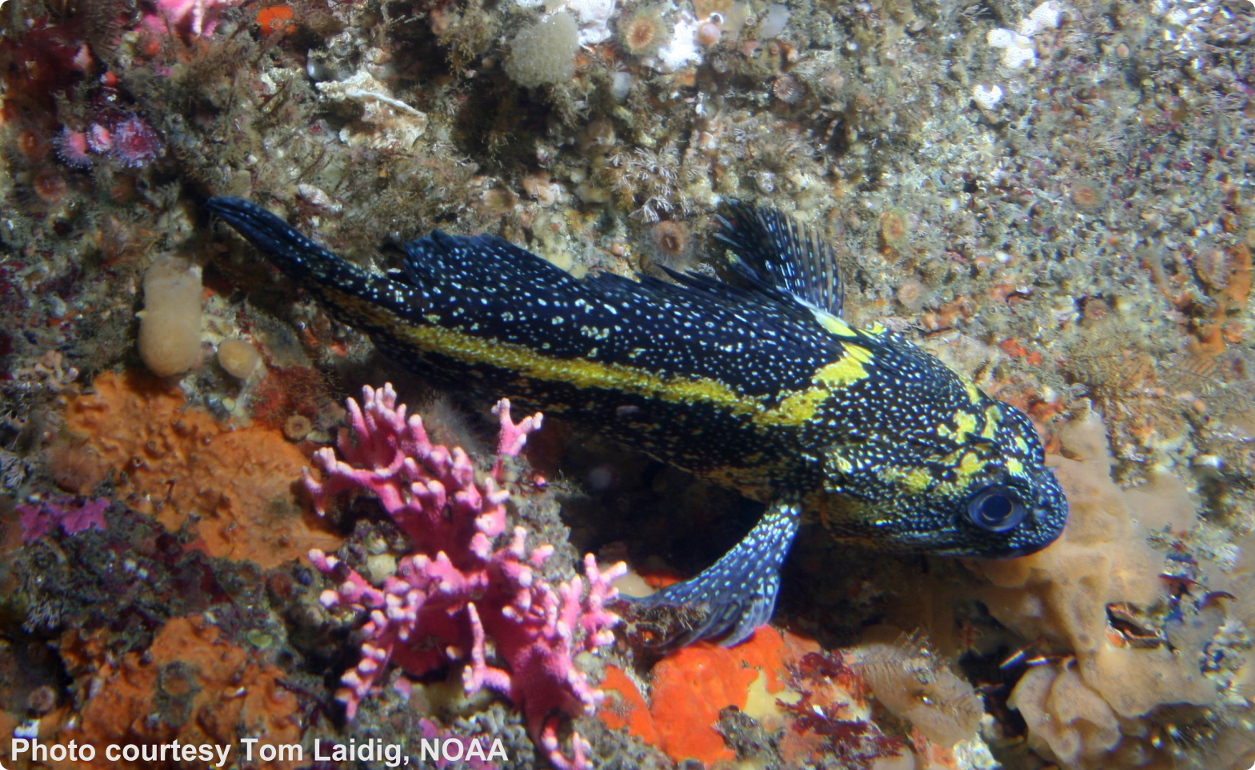
\includegraphics{cover_photo}~\\[1cm]
\pdftooltip{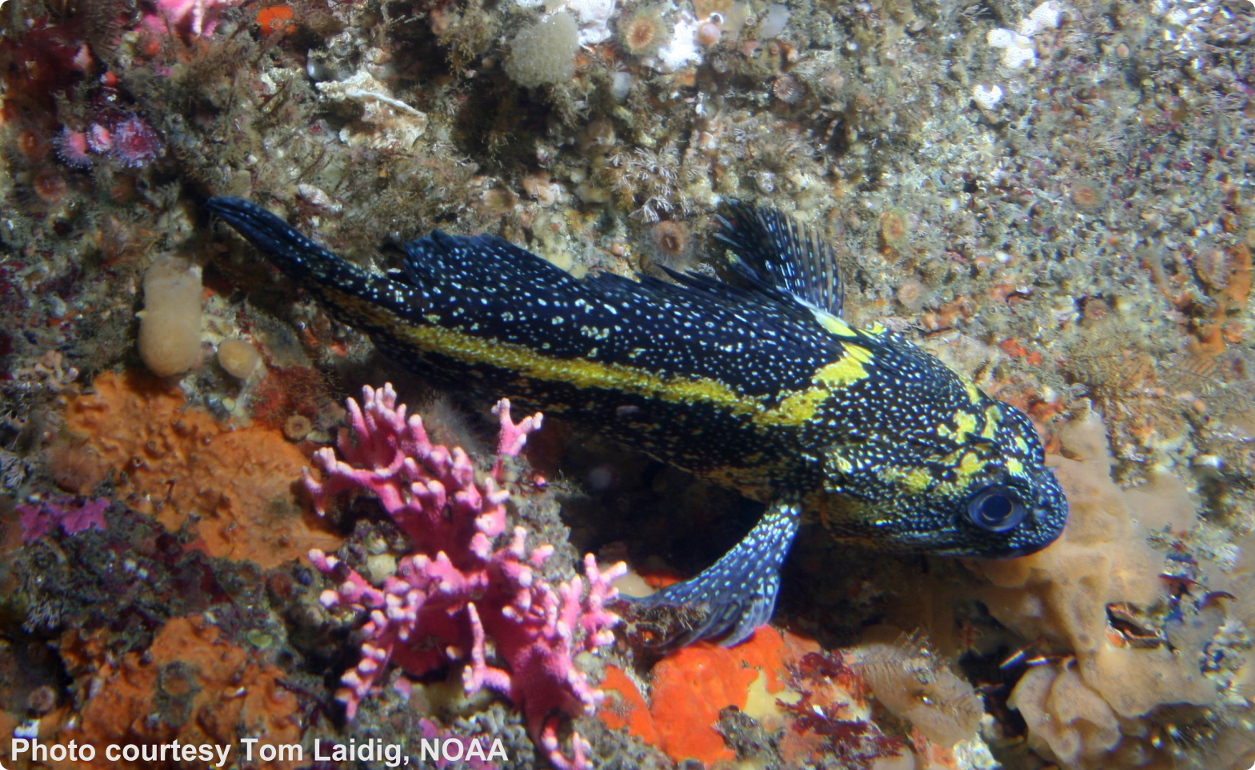
\includegraphics{cover_photo}}{This is a fish.}



E.J. Dick\textsuperscript{1}\\
Author No. 2\textsuperscript{2}\\
Author No. 3\textsuperscript{3}\\

\vspace{.5cm}

\small
\textsuperscript{1}Southwest Fisheries Science Center, U.S. Department of Commerce, National Oceanic and Atmospheric Administration, National Marine Fisheries Service, 110 Shaffer Road, Santa Cruz, California 95060\\

\vspace{.3cm}

\textsuperscript{2}Northwest Fisheries Science Center, U.S. Department of Commerce, National Oceanic and Atmospheric Administration, National Marine Fisheries Service, 2725 Montlake Boulevard East, Seattle, Washington 98112\\

\vspace{.3cm}

\textsuperscript{3}Washington Department of Fish and Wildlife, 600 Capitol Way North, Olympia, Washington 98501\\

\vspace{.3cm}

\textsuperscript{4}Oregon Department of Fish and Wildlife, 2040 SE Marine Science Drive, Newport, OR 97365\\


\vspace{.5cm}

\vfill
DRAFT SAFE\\
Disclaimer: This information is distributed solely for the purpose of pre-dissemination
peer review under applicable information quality guidelines. It has not been formally
disseminated by NOAA Fisheries. It does not represent and should not be construed to
represent any agency determination or policy. 

\vspace{.3cm}
%Bottom of the page
%{\large \today}

\maketitle

\pagenumbering{roman}
\setcounter{page}{1}
\end{center}

{
\setcounter{tocdepth}{4}
\tableofcontents
}
\setlength{\parskip}{5mm plus1mm minus1mm} \pagebreak

\pagenumbering{arabic} \setcounter{page}{1}
\renewcommand{\thefigure}{\alph{figure}}
\renewcommand{\thetable}{\alph{table}}

\section*{Executive Summary}\label{executive-summary}
\addcontentsline{toc}{section}{Executive Summary}

\subsection*{Stock}\label{stock}
\addcontentsline{toc}{subsection}{Stock}

\hl{Include: species/area, including an evaluation of any potential biological basis 
for regional management.}

This assessment reports the status of the China rockfish
(\emph{Sebastes nebulosus}) resource in U.S. waters off the coast of the
California, Oregon, and Washington using data through 2013. Etc\ldots{}

\subsection*{Catches}\label{catches}
\addcontentsline{toc}{subsection}{Catches}

\hl{Include: trends and current levels-include table for last ten years and graph with 
long term data}

Catch figure(s) with fleets: (Figures
\ref{fig:Exec_catch1}-\ref{fig:Exec_catch3})\\
Catch table: (Table \ref{tab:Exec_catch})

\FloatBarrier

\begin{figure}[htbp]
\centering
\includegraphics{Assessment_template_files/figure-latex/unnamed-chunk-2-1.pdf}
\caption{China rockfish landings in \ldots{}.. \label{fig:Exec_catch1}}
\end{figure}

\begin{figure}[htbp]
\centering
\includegraphics{Assessment_template_files/figure-latex/unnamed-chunk-3-1.pdf}
\caption{Stacked line plot of China rockfish landings history for Oregon
by fleet (recreational and commercial). \label{fig:Exec_catch2}}
\end{figure}

\begin{figure}[htbp]
\centering
\includegraphics{Assessment_template_files/figure-latex/unnamed-chunk-4-1.pdf}
\caption{Stacked line plot of China rockfish landings history for
California by fleet (recreational and commercial).
\label{fig:Exec_catch3}}
\end{figure}

\begin{figure}[htbp]
\centering
\includegraphics{r4ss/plots_mod1/catch2\%20landings\%20stacked.png}
\caption{Landings history of China rockfish. \label{fig:r4ss_catches}}
\end{figure}

\begin{table}[ht]
\centering
\caption{Recent China rockfish landings (mt) by 
                                            fleet.} 
\label{tab:Exec_catch}
\begin{tabular}{l>{\centering}p{1in}>{\centering}p{1in}>{\centering}p{1in}>{\centering}p{.9in}>{\centering}p{.9in}>{\centering}p{.6in}}
  \hline
Year & Landings 1 & Landings 2 & Landings 3 & Landings 4 & Landings 5 & Total \\ 
  \hline
2005 & - & - & - & - & - & - \\ 
  2006 & - & - & - & - & - & - \\ 
  2007 & - & - & - & - & - & - \\ 
  2008 & - & - & - & - & - & - \\ 
  2009 & - & - & - & - & - & - \\ 
  2010 & - & - & - & - & - & - \\ 
  2011 & - & - & - & - & - & - \\ 
  2012 & - & - & - & - & - & - \\ 
  2013 & - & - & - & - & - & - \\ 
  2014 & - & - & - & - & - & - \\ 
   \hline
\end{tabular}
\end{table}

\FloatBarrier

\newpage

\subsection*{Data and Assessment}\label{data-and-assessment}
\addcontentsline{toc}{subsection}{Data and Assessment}

\hl{Include: date of last assessment, type of assessment model, data available, new 
information, and information lacking.}

China rockfish was assessed\ldots{}. This assessment uses the newest
version of Stock Synthesis (3.24u). The model begins in 1900, and
assumes the stock was at an unfished equilibrium that year.

Map of assessment region: (Figure \ref{fig:assess_region_map}).

\begin{figure}[htbp]
\centering
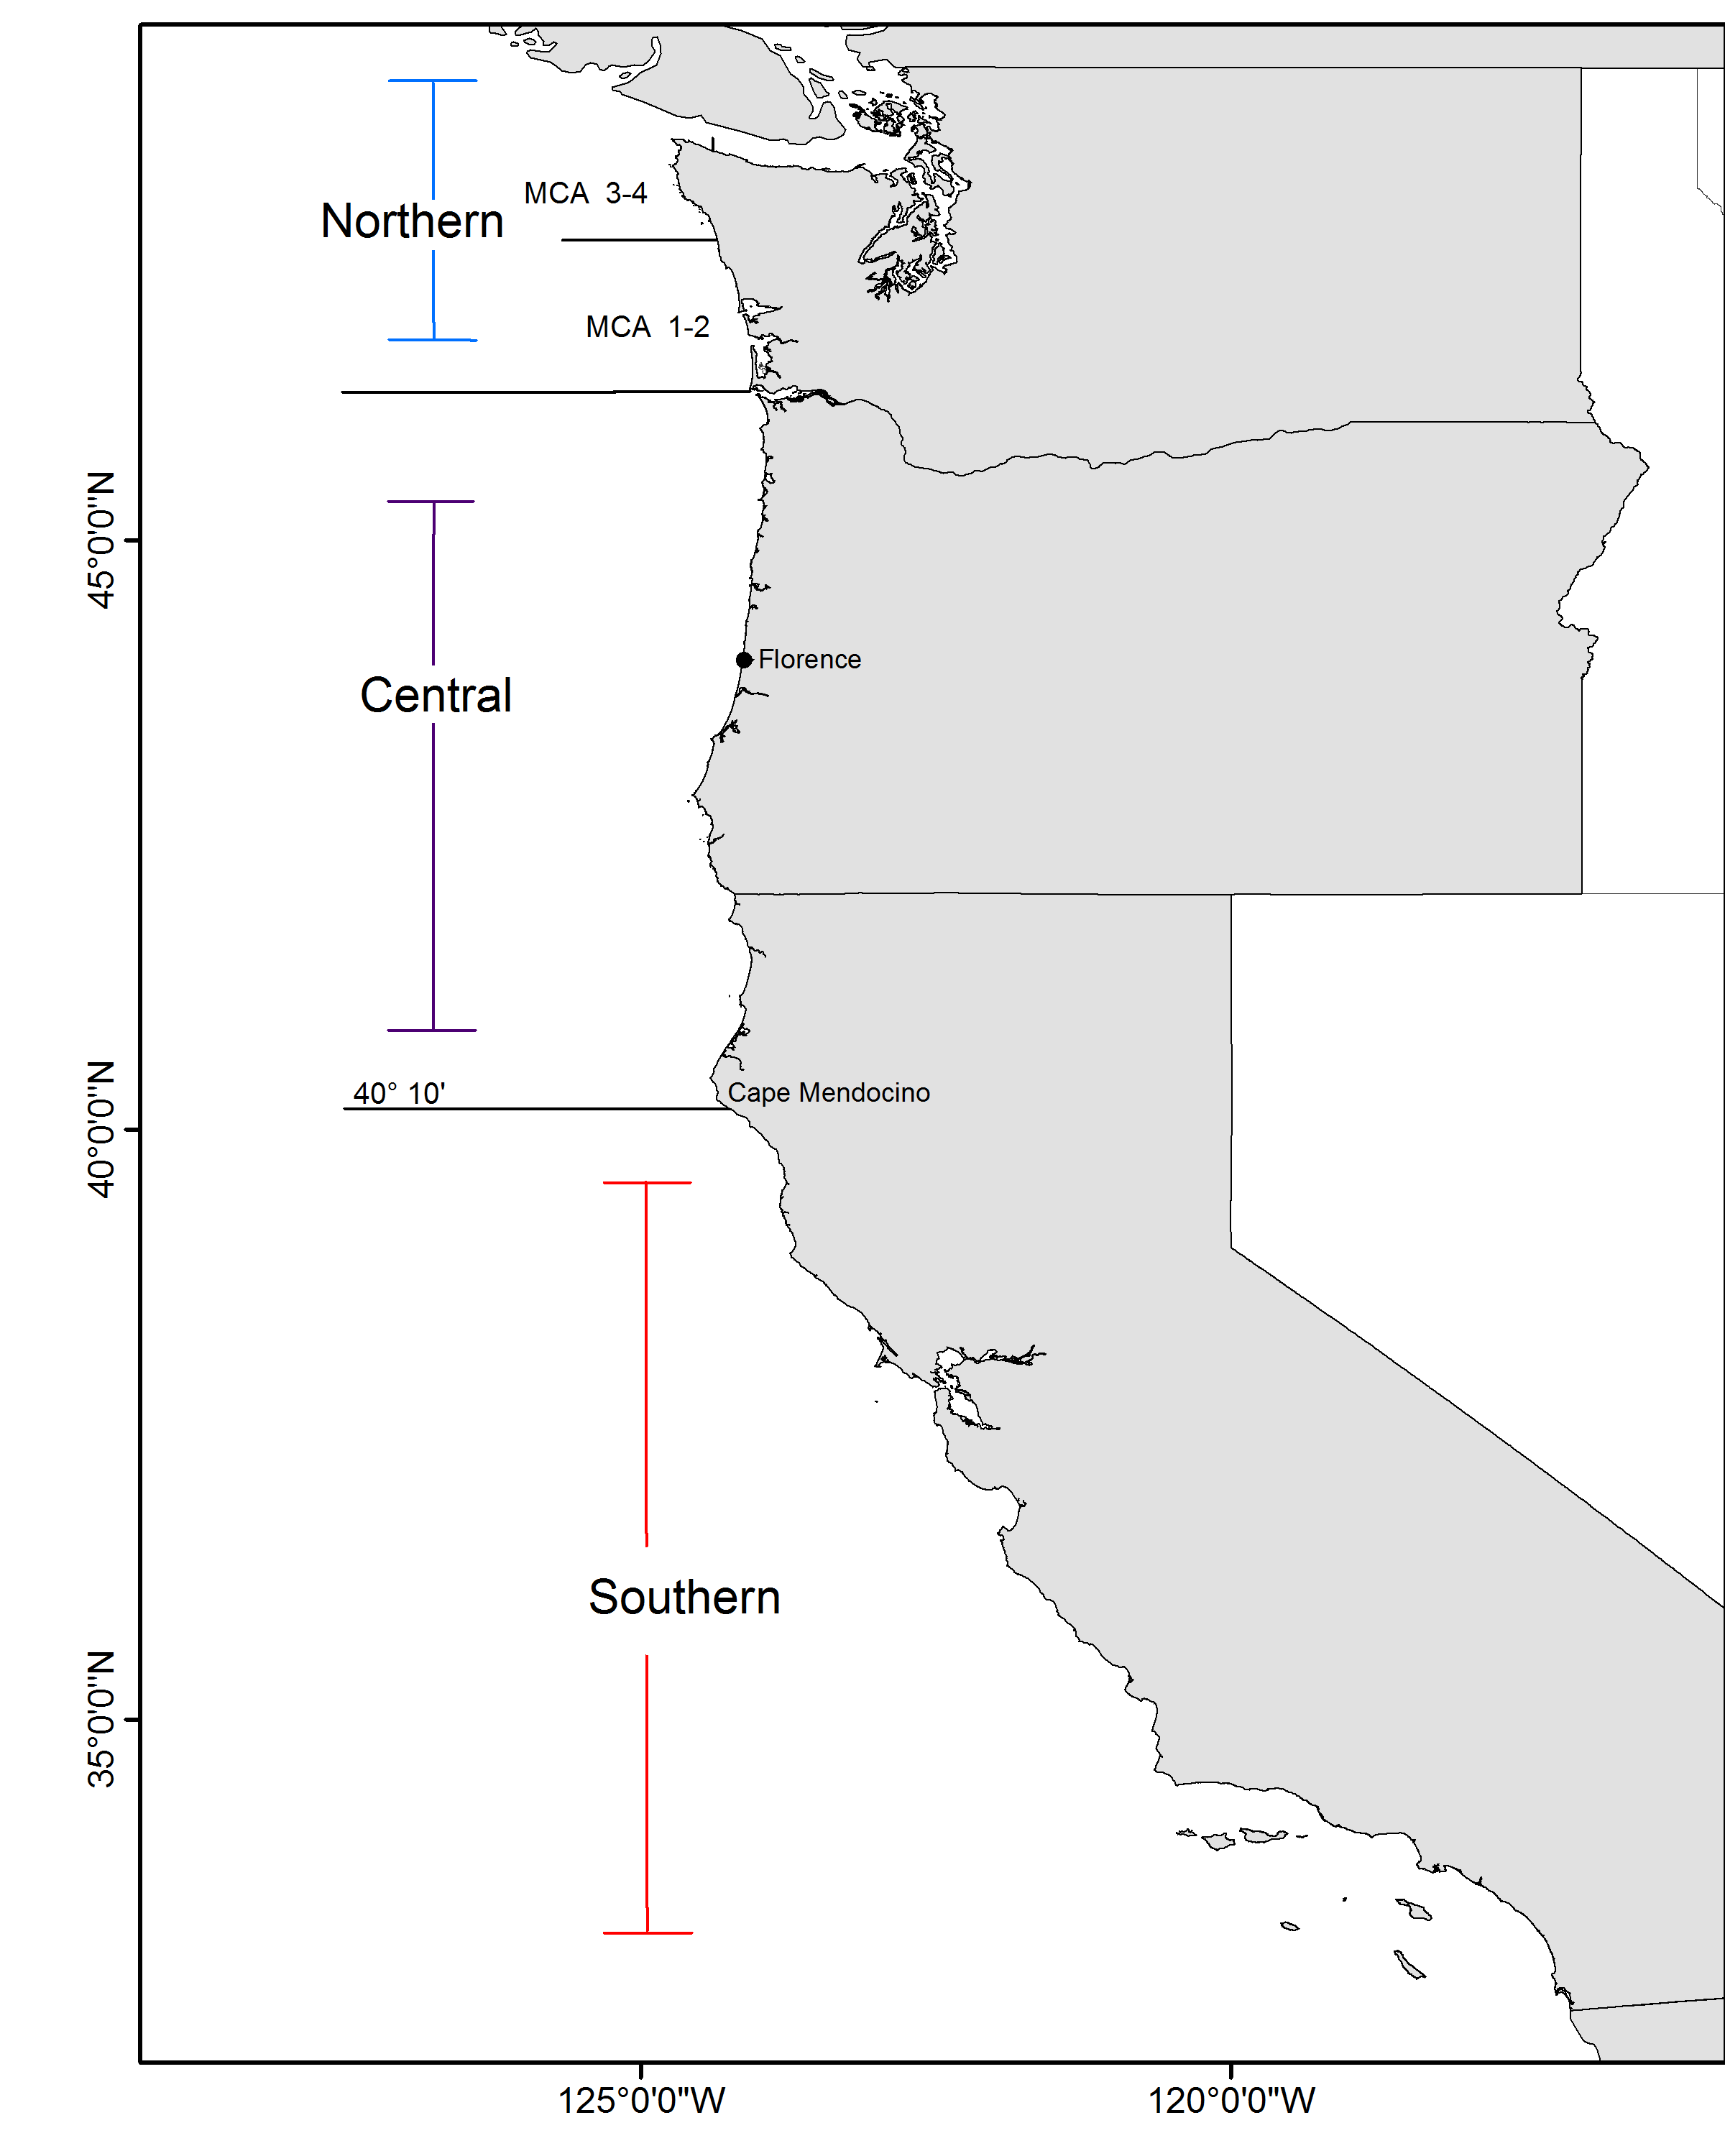
\includegraphics{Figures/assess_region_map.png}
\caption{Map depicting the boundaries for the base-case model.
\label{fig:assess_region_map}}
\end{figure}

\FloatBarrier

\subsection*{Stock Biomass}\label{stock-biomass}
\addcontentsline{toc}{subsection}{Stock Biomass}

\hl{Include: trends and current levels relative to virgin or historic levels, 
description of uncertainty-include table for last 10 years and graph with 
long term estimates.}

Spawning output Figure: Figure \ref{fig:Spawnbio_all}\\
Spawning output Table(s): Table \ref{tab:SpawningDeplete_mod1}\\
Relative depletion Figure: Figure \ref{fig:RelDeplete_all}

Example text (remove Models 2 and 3 if not needed - if using, remove the
\# in-line comments!!!)\\
The estimated relative depletion level (spawning output relative to
unfished spawning output) of the the base-case model in 2014 is 73.4\%
(\textasciitilde{}95\% asymptotic interval: \(\pm\) 63.7\%-83.2\%)
(Figure \ref{fig:RelDeplete_all}).

The estimated relative depletion level of model 2 in 2014 is
(\textasciitilde{}95\% asymptotic interval: \(\pm\) ) (Figure
\ref{fig:RelDeplete_all}).

The estimated relative depletion level of model 3 in 2014 is
(\textasciitilde{}95\% asymptotic interval: \(\pm\) ) (Figure
\ref{fig:RelDeplete_all}).

\FloatBarrier

\begin{table}[ht]
\centering
\caption{Recent trend in beginning of the 
                                      year spawning output and depletion for
                                      the base model for China rockfish.} 
\label{tab:SpawningDeplete_mod1}
\begin{tabular}{l>{\centering}p{1.3in}>{\centering}p{1.2in}>{\centering}p{1in}>{\centering}p{1.2in}}
  \hline
Year & Spawning Output (billion eggs) & \~{} 95\% confidence interval & Estimated depletion & \~{} 95\% confidence interval \\ 
  \hline
2005 & 17.891 & (8.81-26.97) & 0.732 & (0.635-0.829) \\ 
  2006 & 17.942 & (8.86-27.03) & 0.734 & (0.638-0.83) \\ 
  2007 & 18.030 & (8.94-27.12) & 0.738 & (0.642-0.833) \\ 
  2008 & 18.044 & (8.95-27.14) & 0.738 & (0.643-0.833) \\ 
  2009 & 18.034 & (8.93-27.13) & 0.738 & (0.642-0.833) \\ 
  2010 & 18.062 & (8.96-27.17) & 0.739 & (0.644-0.834) \\ 
  2011 & 17.993 & (8.89-27.1) & 0.736 & (0.64-0.833) \\ 
  2012 & 17.971 & (8.86-27.08) & 0.735 & (0.638-0.832) \\ 
  2013 & 17.981 & (8.87-27.09) & 0.736 & (0.639-0.833) \\ 
  2014 & 17.944 & (8.83-27.06) & 0.734 & (0.637-0.832) \\ 
   \hline
\end{tabular}
\end{table}

\FloatBarrier

\begin{figure}[htbp]
\centering
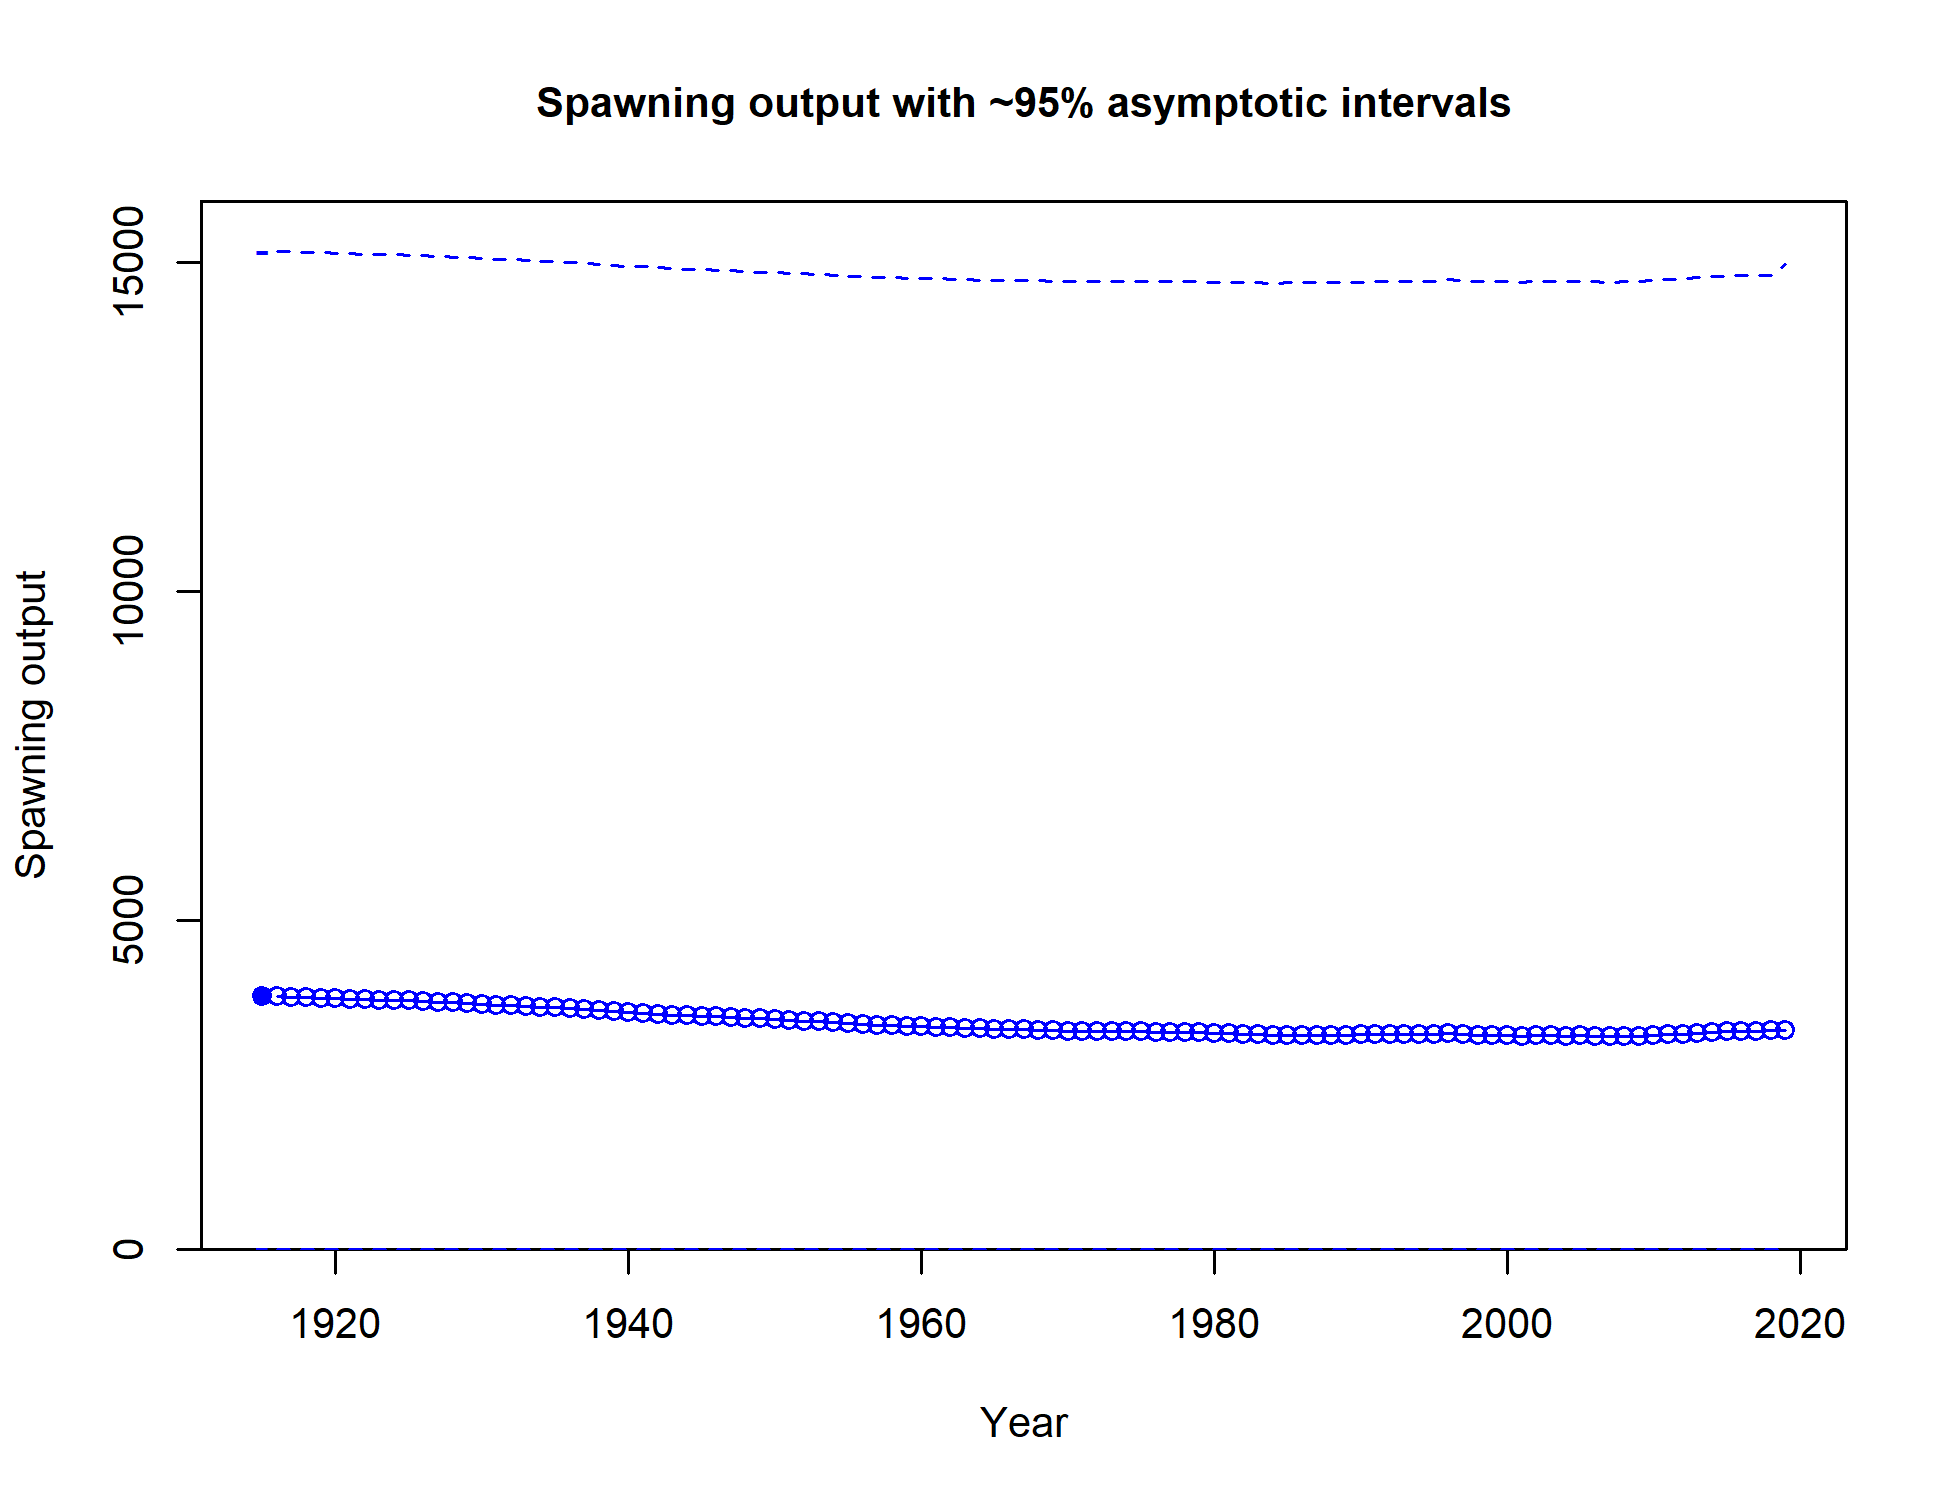
\includegraphics{r4ss/plots_mod1/ts7_Spawning_output_with_95_asymptotic_intervals_intervals.png}
\caption{Time series of spawning output trajectory (circles and line:
median; light broken lines: 95\% credibility intervals) for the base
case assessment model. \label{fig:Spawnbio_all}}
\end{figure}

\begin{figure}[htbp]
\centering
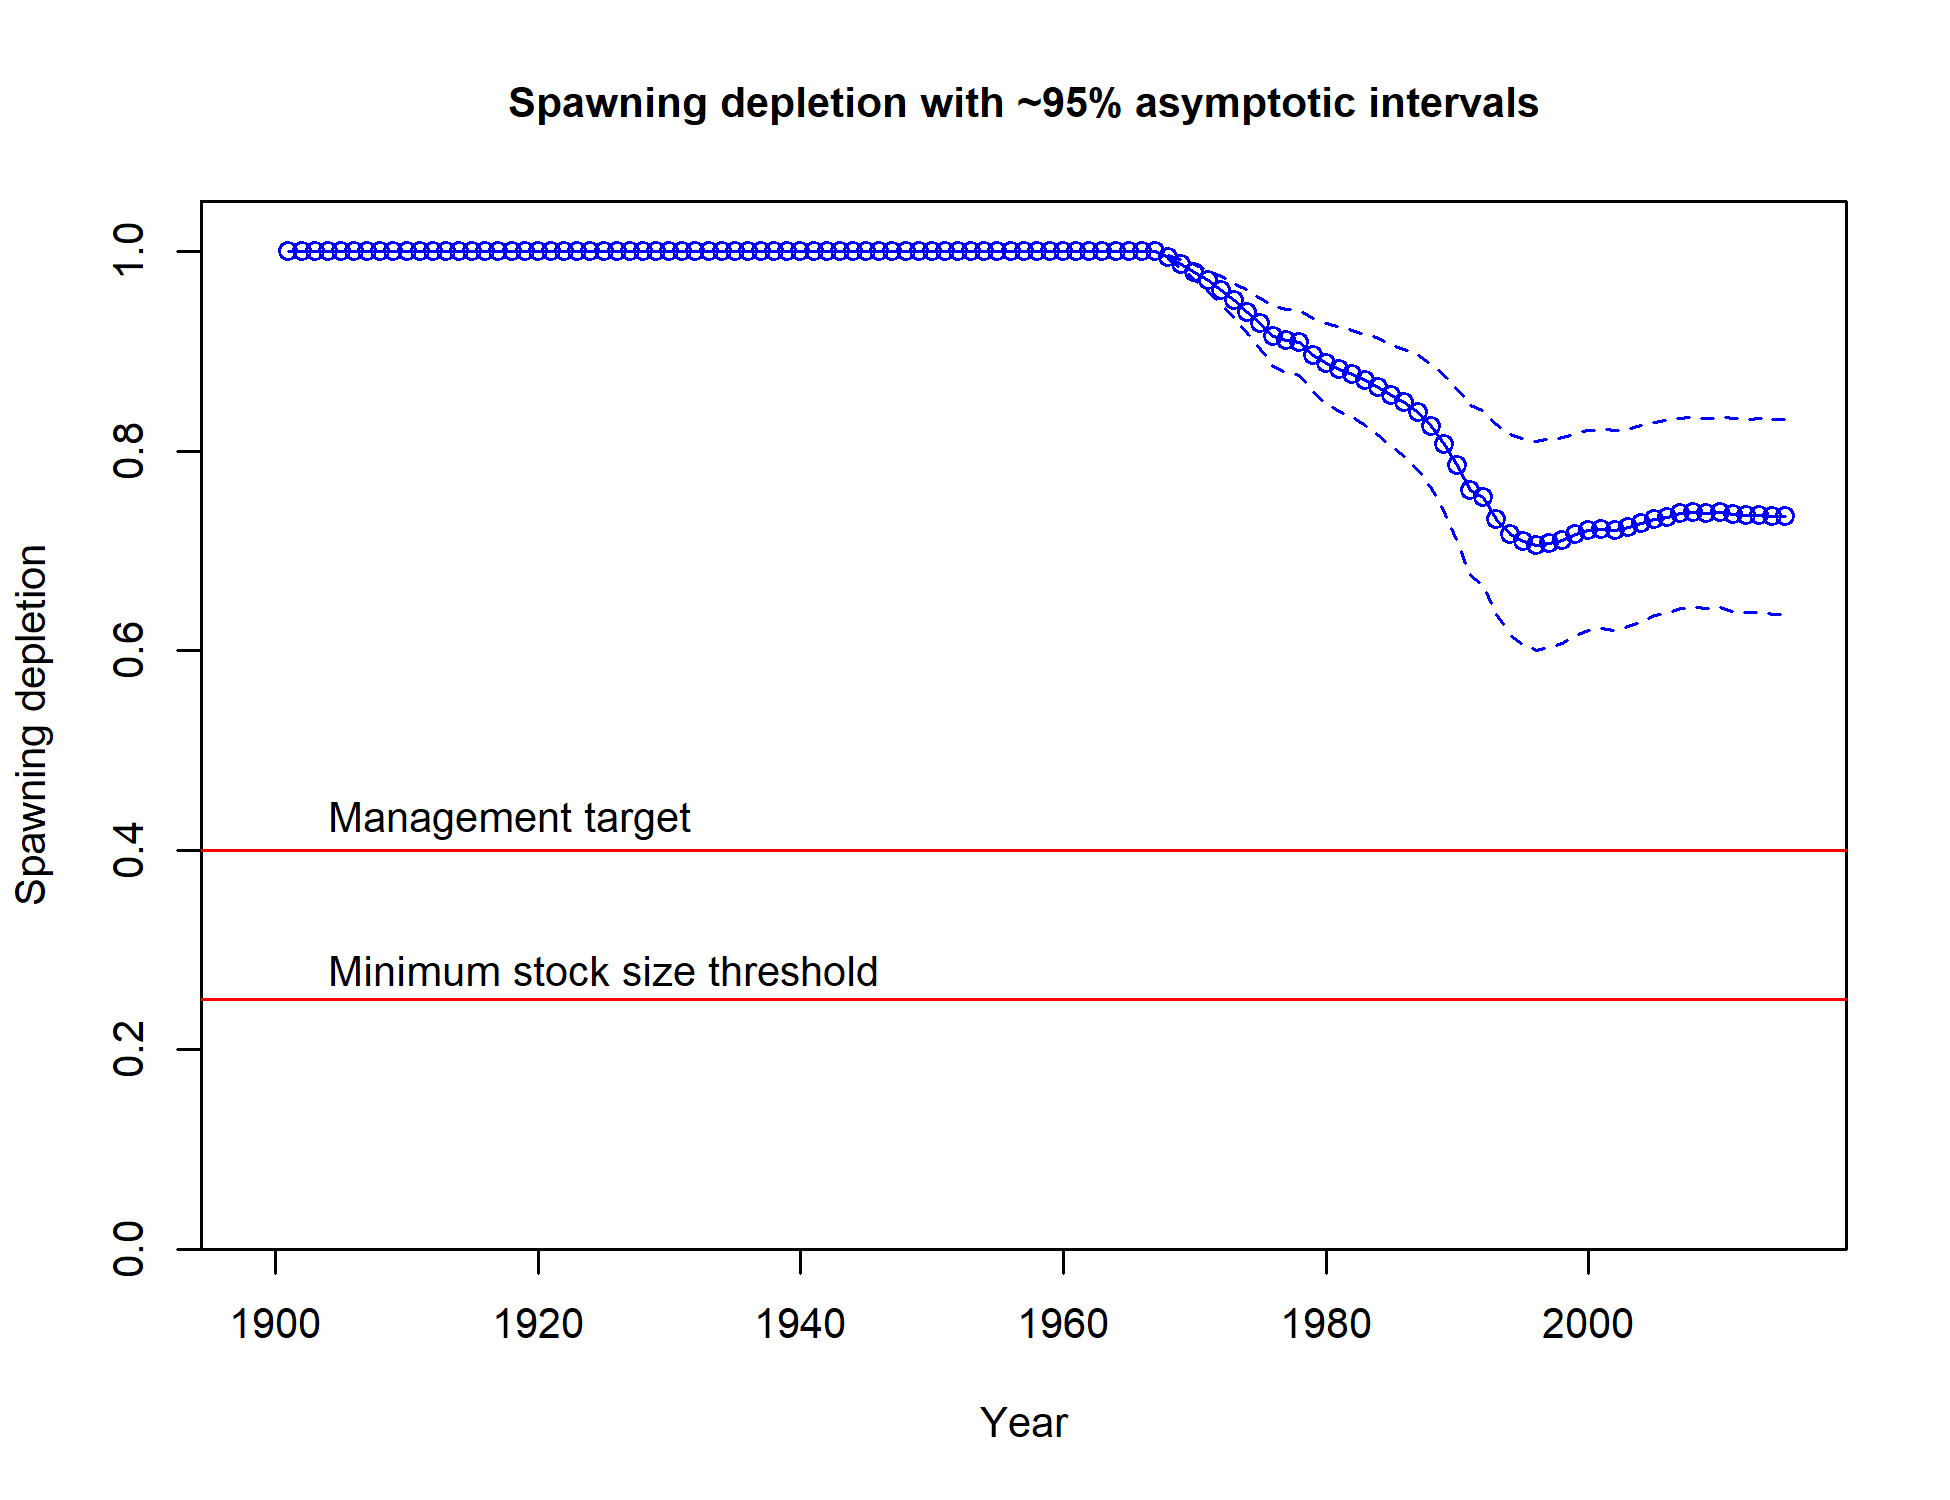
\includegraphics{r4ss/plots_mod1/ts9_Spawning_depletion_with_95_asymptotic_intervals_intervals.png}
\caption{Estimated relative depletion with approximate 95\% asymptotic
confidnce intervals (dashed lines) for the base case assessment model.
\label{fig:RelDeplete_all}}
\end{figure}

\FloatBarrier

\subsection*{Recruitment}\label{recruitment}
\addcontentsline{toc}{subsection}{Recruitment}

\hl{Include: trends and current levels relative to virgin or historic levels-include 
table for last 10 years and graph with long term estimates.}

Recruitment Figure: (Figure \ref{fig:Recruits_all})\\
Recruitment Tables: (Tables \ref{tab:Recruit_mod1},
\ref{tab:Recruit_mod2} and \ref{tab:Recruit_mod3})

\begin{table}[ht]
\centering
\caption{Recent recruitment for the base model.} 
\label{tab:Recruit_mod1}
\begin{tabular}{rrl}
  \hline
Year & Estimated Recruitment (1,000s) & \~{} 95\% confidence interval \\ 
  \hline
2005 & 33.28 & (21.32 - 45.23) \\ 
  2006 & 33.29 & (21.33 - 45.24) \\ 
  2007 & 33.30 & (21.35 - 45.25) \\ 
  2008 & 33.30 & (21.35 - 45.26) \\ 
  2009 & 33.30 & (21.35 - 45.26) \\ 
  2010 & 33.31 & (21.35 - 45.26) \\ 
  2011 & 33.30 & (21.34 - 45.25) \\ 
  2012 & 33.29 & (21.33 - 45.25) \\ 
  2013 & 33.29 & (21.33 - 45.25) \\ 
  2014 & 33.29 & (21.33 - 45.25) \\ 
   \hline
\end{tabular}
\end{table}

\FloatBarrier

\begin{figure}[htbp]
\centering
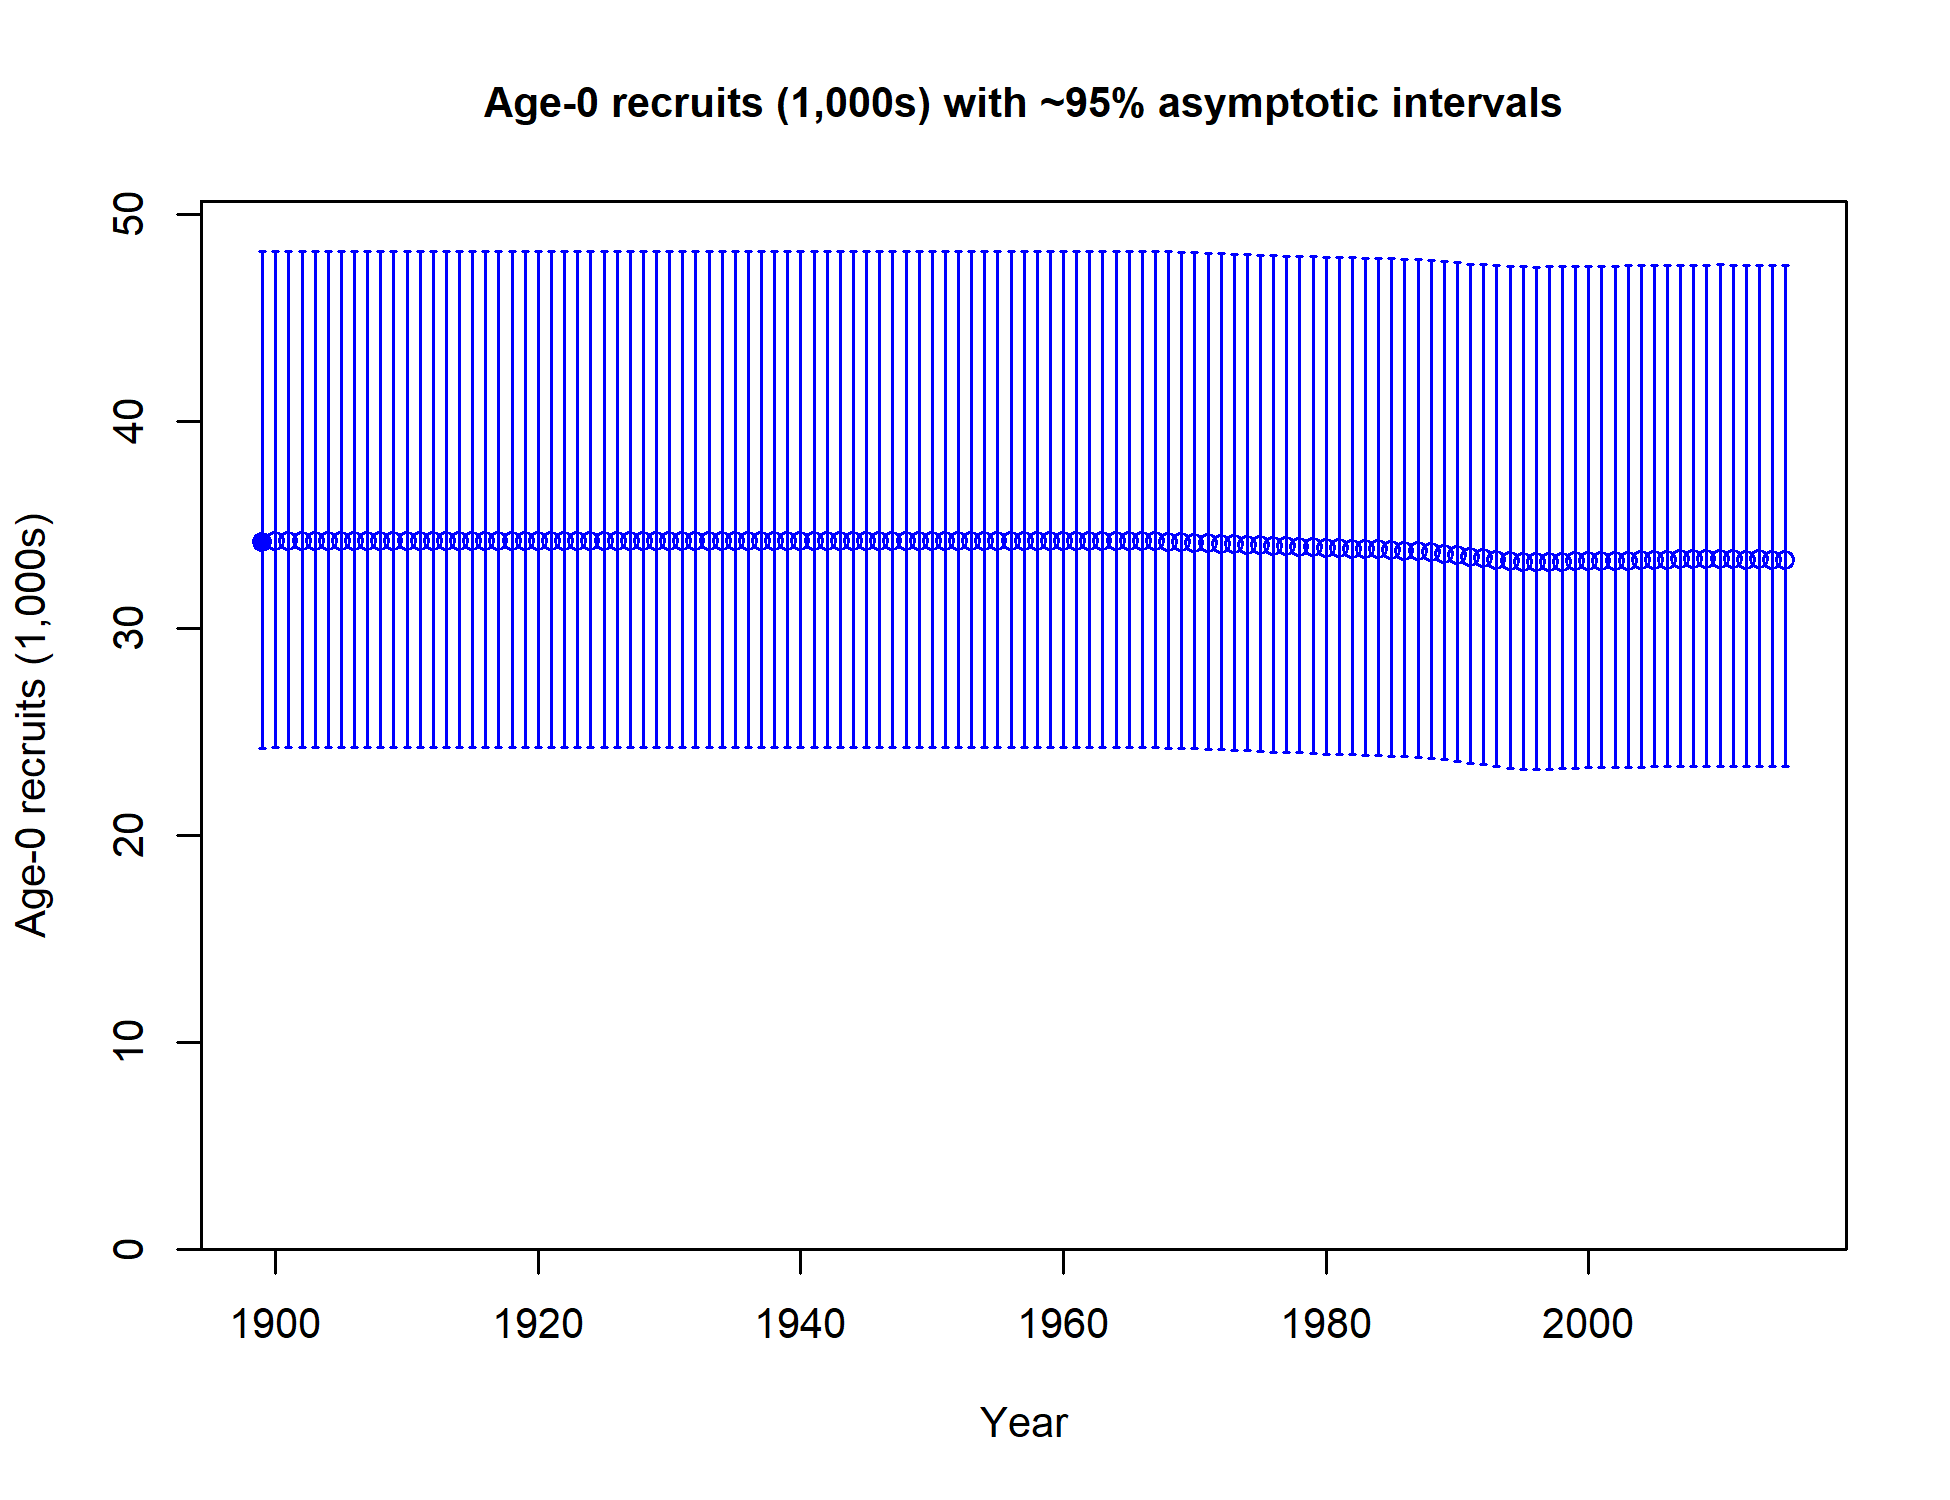
\includegraphics{r4ss/plots_mod1/ts11_Age-0_recruits_(1000s)_with_95_asymptotic_intervals.png}
\caption{Time series of estimated China rockfish recruitments for the
base-case model with 95\% confidence or credibility intervals.
\label{fig:Recruits_all}}
\end{figure}

\FloatBarrier

\subsection*{Exploitation status}\label{exploitation-status}
\addcontentsline{toc}{subsection}{Exploitation status}

\hl{Include: exploitation rates (i.e., total catch divided by exploitable biomass, or the annual SPR harvest rate) – include a table with the last 10 years of data and a graph showing the trend in fishing mortality relative to the target (y-axis) plotted against the trend in biomass relative to the target (x-axis).}

Exploitation Tables: Table \ref{tab:SPR_Exploit_mod1}, Table
\ref{tab:SPR_Exploit_mod2}, Table \ref{tab:SPR_Exploit_mod3}
Exploitation Figure: Figure \ref{fig:SPR_all}).

A summary of China rockfish exploitation histories for base model is
provided as Figure \ref{fig:Phase_all}.

\FloatBarrier

\begin{table}[ht]
\centering
\caption{Recent trend in spawning potential 
                                        ratio and exploitation for China rockfish in the base model.  Fishing intensity is (1-SPR) 
                                        divided by 50\% (the SPR target) and exploitation 
                                        is F divided by F\textsubscript{SPR}.} 
\label{tab:SPR_Exploit_mod1}
\begin{tabular}{l>{\centering}p{1in}>{\centering}p{1.2in}>{\centering}p{1in}>{\centering}p{1.2in}}
  \hline
Year & Fishing intensity & \~{} 95\% confidence interval & Exploitation rate & \~{} 95\% confidence interval \\ 
  \hline
2004 & 0.39 & (0.23-0.54) & 0.27 & (0.14-0.39) \\ 
  2005 & 0.44 & (0.27-0.61) & 0.32 & (0.17-0.47) \\ 
  2006 & 0.39 & (0.24-0.55) & 0.28 & (0.15-0.4) \\ 
  2007 & 0.47 & (0.3-0.65) & 0.35 & (0.19-0.51) \\ 
  2008 & 0.50 & (0.32-0.68) & 0.38 & (0.2-0.55) \\ 
  2009 & 0.45 & (0.28-0.63) & 0.33 & (0.18-0.49) \\ 
  2010 & 0.56 & (0.36-0.76) & 0.44 & (0.24-0.64) \\ 
  2011 & 0.51 & (0.32-0.7) & 0.39 & (0.21-0.57) \\ 
  2012 & 0.48 & (0.3-0.66) & 0.35 & (0.19-0.52) \\ 
  2013 & 0.53 & (0.34-0.72) & 0.41 & (0.22-0.59) \\ 
   \hline
\end{tabular}
\end{table}

\FloatBarrier

\begin{figure}[htbp]
\centering
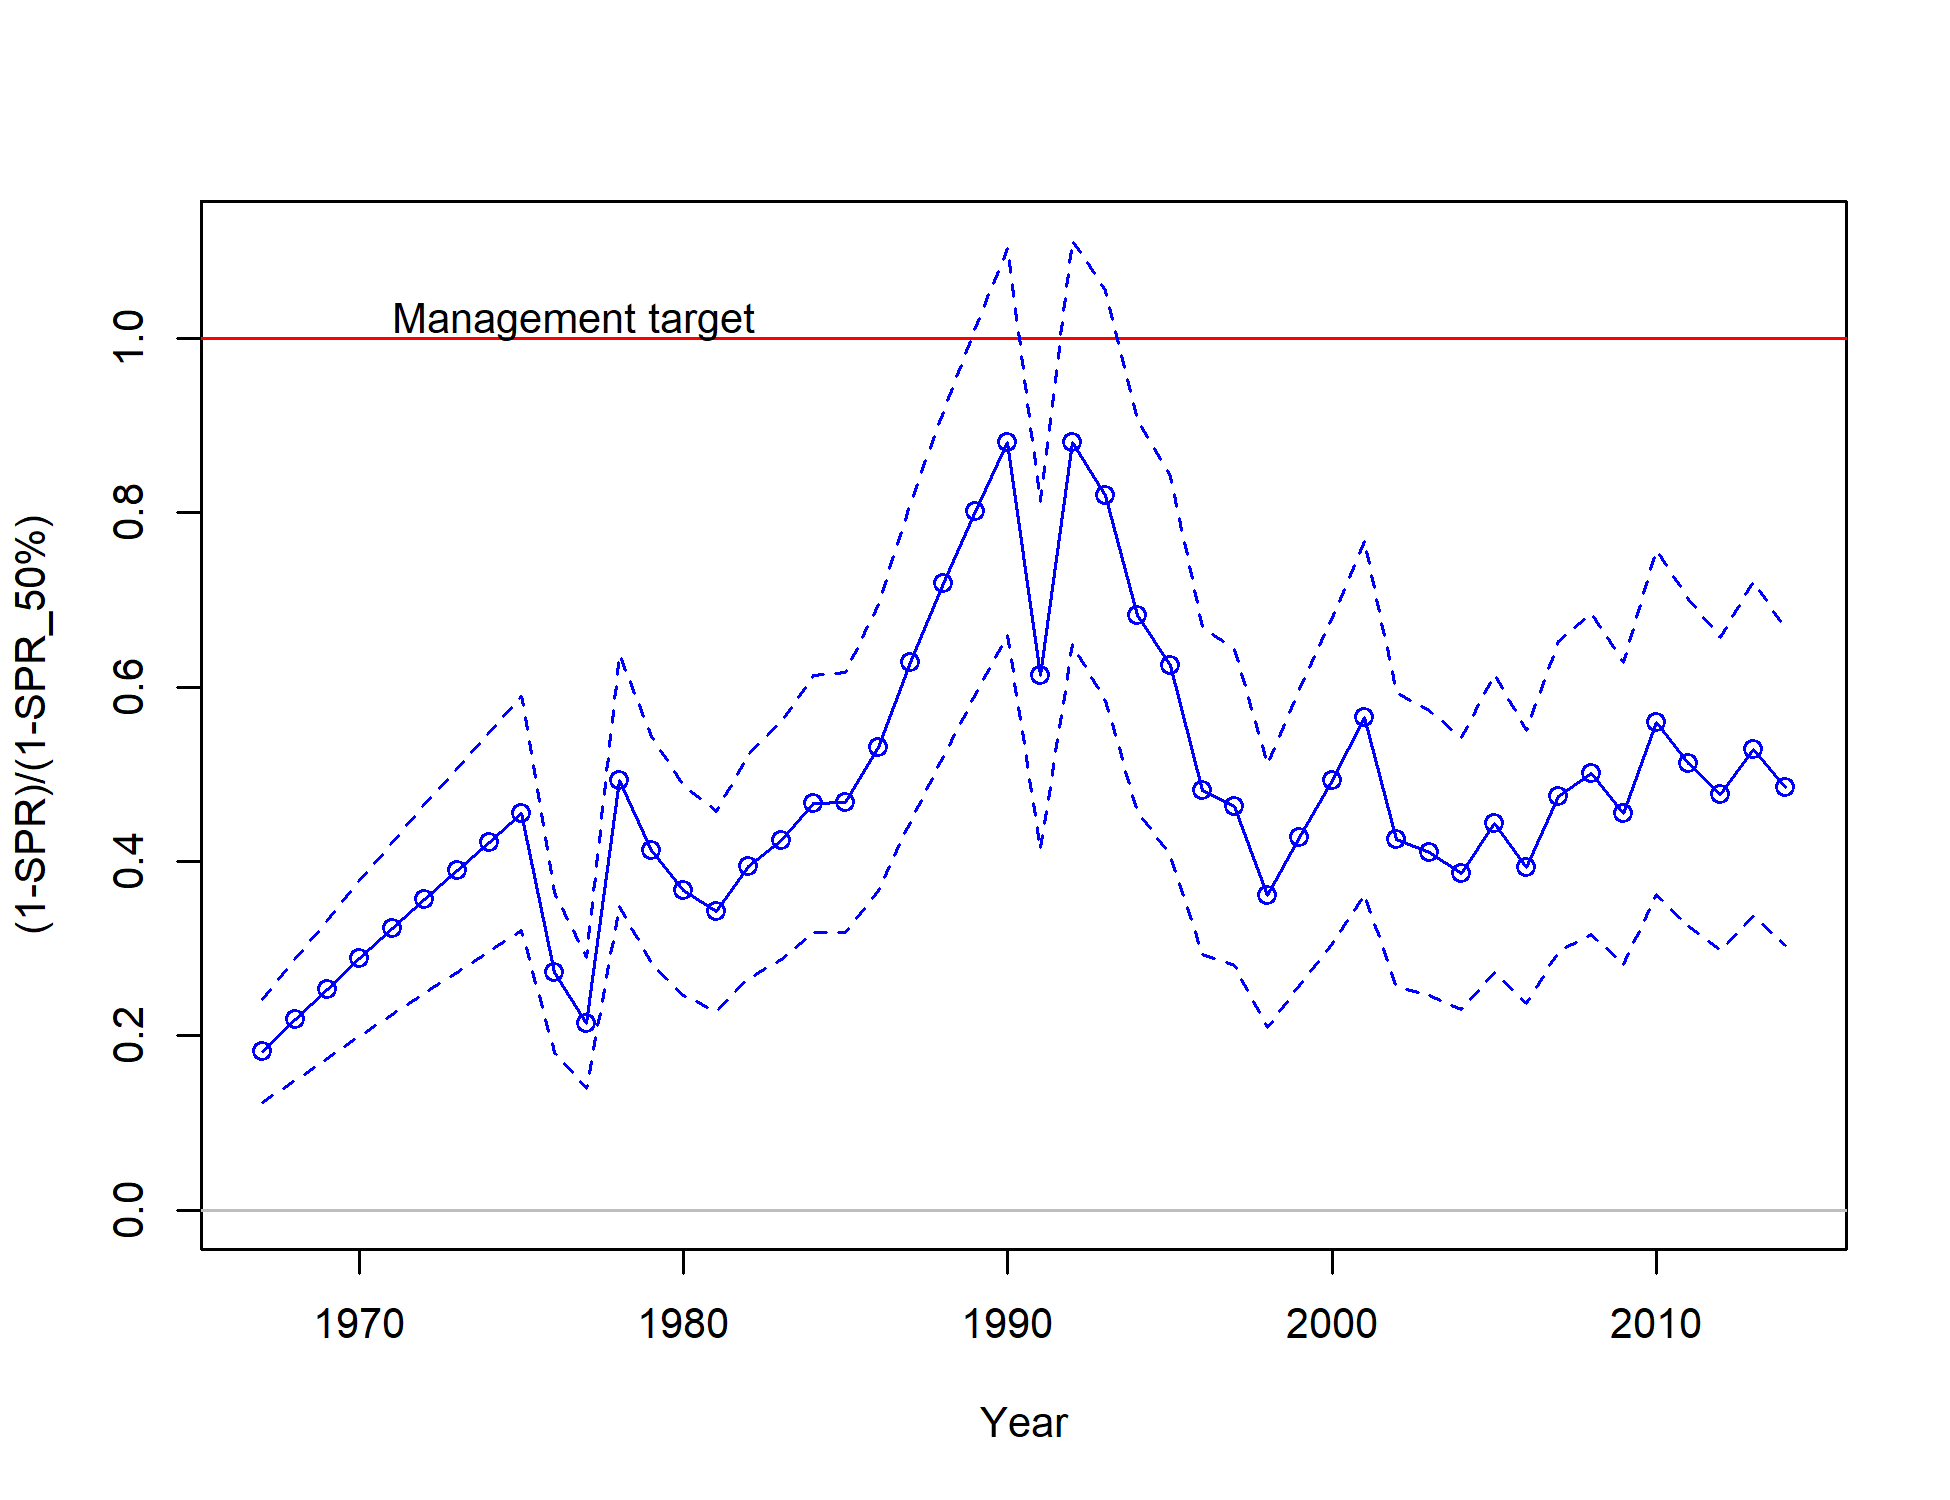
\includegraphics{r4ss/plots_mod1/SPR3_ratiointerval.png}
\caption{Estimated spawning potential ratio (SPR) for the base-case
model. One minus SPR is plotted so that higher exploitation rates occur
on the upper portion of the y-axis. The management target is plotted as
a red horizontal line and values above this reflect harvests in excess
of the overfishing proxy based on the SPR\textsubscript{50\%} harvest
rate. The last year in the time series is 2014. \label{fig:SPR_all}}
\end{figure}

\begin{figure}[htbp]
\centering
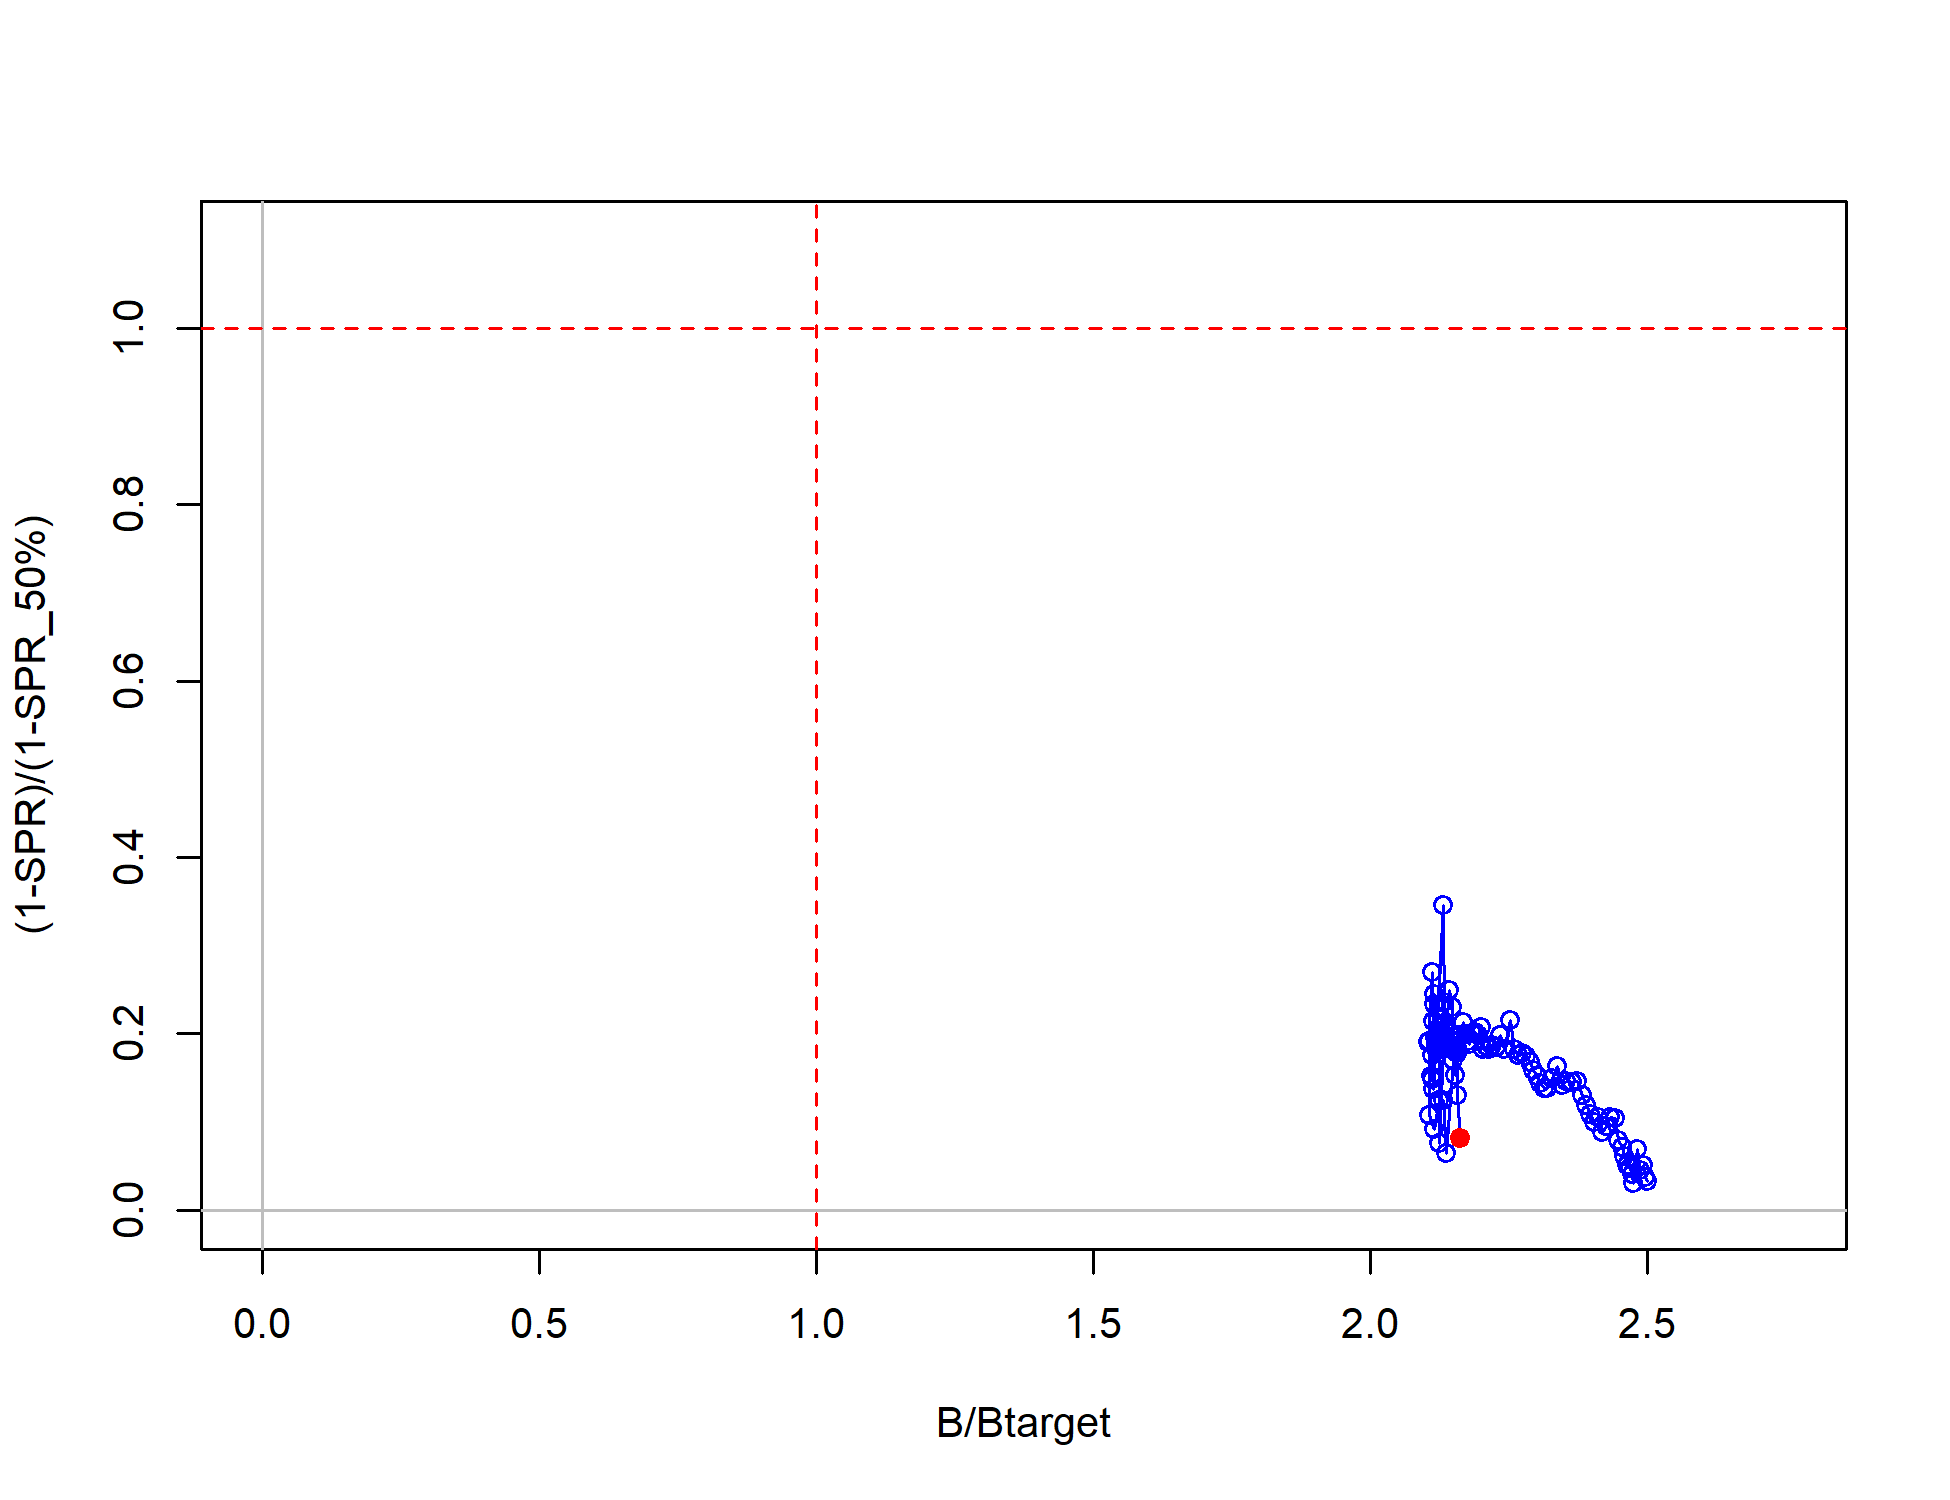
\includegraphics{r4ss/plots_mod1/SPR4_phase.png}
\caption{Phase plot of estimated relative (1-SPR) vs.~relative spawning
biomass for the base case model. The relative (1-SPR) is (1-SPR) divided
by 50\% (the SPR target). Relative depletion is the annual spawning
biomass divided by the unfished spawning biomass. \label{fig:Phase_all}}
\end{figure}

\FloatBarrier

\subsection*{Ecosystem Considerations}\label{ecosystem-considerations}
\addcontentsline{toc}{subsection}{Ecosystem Considerations}

In this assessment, ecosystem considerations were\ldots{}..

\subsection*{Reference Points}\label{reference-points}
\addcontentsline{toc}{subsection}{Reference Points}

\hl{Include:} management targets and definition of overfishing,
including the harvest rate that brings the stock to equilibrium at
\(B_{40\%}\) (the \(B_{MSY}\) proxy) and the equilibrium stock size that
results from fishing at the default harvest rate (the \(F_{MSY}\)
proxy). Include a summary table that compares estimated reference points
for SSB, SPR, Exploitation Rate and Yield based on SSBproxy for MSY,
SPRproxy for MSY, and estimated MSY values

\hl{Write intro paragraph....and remove text for Models 2 and 3 if not needed}

This stock assessment estimates that China rockfish in the base model
are above the biomass target, but above the minimum stock size
threshold. \hl{Add sentence about spawning output trend.} The estimated
relative depletion level for \hl{Model 1} in 2014 is 73.4\%
(\textasciitilde{}95\% asymptotic interval: \(\pm\) 63.7\%-83.2\%,
corresponding to an unfished spawning output of 17.9443 billion eggs
(\textasciitilde{}95\% asymptotic interval: 8.83-27.06 billion eggs) of
spawning output in the base model (Table \ref{tab:Ref_pts_mod1}).
Unfished age 1+ biomass was estimated to be 240.8 mt in the base case
model. The target spawning output based on the biomass target
(\(SB_{40\%}\)) is 9.8 billion eggs, which gives a catch of 6.3 mt.
Equilibrium yield at the proxy \(F_{MSY}\) harvest rate corresponding to
\(SPR_{50\%}\) is 5.8 mt.

This stock assessment estimates that China rockfish in the are

the biomass target, but\\
the minimum stock size threshold.
\hl{Add sentence about spawning output trend.} The estimated relative
depletion level for \hl{Model 2} in 2014 is (\textasciitilde{}95\%
asymptotic interval: \(\pm\) ), corresponding to an unfished spawning
output of (\textasciitilde{}95\% asymptotic interval: ) of spawning
output in the base model (Table \ref{tab:Ref_pts_mod2}). Unfished age 1+
biomass was estimated to be\\
mt in the base case model. The target spawning output based on the
biomass target (\(SB_{40\%}\)) is , which gives a catch of mt.
Equilibrium yield at the proxy \(F_{MSY}\) harvest rate corresponding to
\(SPR_{50\%}\) is mt.

This stock assessment estimates that China rockfish in the are

the biomass target, but\\
the minimum stock size threshold.
\hl{Add sentence about spawning output trend.} The estimated relative
depletion level or \hl{Model 3} in 2014 is (\textasciitilde{}95\%
asymptotic interval: \(\pm\) ), corresponding to an unfished spawning
output of (\textasciitilde{}95\% asymptotic interval: ) of spawning
output in the base model (Table \ref{tab:Ref_pts_mod3}). Unfished age 1+
biomass was estimated to be mt in the base case model. The target
spawning output based on the biomass target (\(SB_{40\%}\)) is , which
gives a catch of mt. Equilibrium yield at the proxy \(F_{MSY}\) harvest
rate corresponding to \(SPR_{50\%}\) is mt.

\FloatBarrier

\begin{table}[ht]
\centering
\caption{Summary of reference 
                                      points and management quantities for the 
                                      base case base model.} 
\label{tab:Ref_pts_mod1}
\begin{tabular}{>{\raggedright}p{4.1in}>{\centering}p{.65in}>{\centering}p{1.4in}}
  \hline
\textbf{Quantity} & \textbf{Estimate} & \textbf{\~95\%  Confidence Interval} \\ 
  \hline
Unfished spawning output (billion eggs) & 24.4 & (15.2-33.7) \\ 
  Unfished age 1+ biomass (mt) & 240.8 & (153-328.7) \\ 
  Unfished recruitment (R0, thousands) & 34.2 & (22.3-46) \\ 
  Spawning output(2014 billion eggs) & 17.9 & (8.8-27.1) \\ 
  Depletion (2014) & 0.7342 & (0.6367-0.8317) \\ 
  \textbf{$\text{Reference points based on } \mathbf{SB_{40\%}}$} &  &  \\ 
  Proxy spawning output ($B_{40\%}$) & 9.8 & (6.1-13.5) \\ 
  SPR resulting in $B_{40\%}$ ($SPR_{B40\%}$) & 0.444 & (0.444-0.444) \\ 
  Exploitation rate resulting in $B_{40\%}$ & 0.0551 & (0.0522-0.058) \\ 
  Yield with $SPR_{B40\%}$ at $B_{40\%}$ (mt) & 6.3 & (4-8.5) \\ 
  \textbf{\textit{Reference points based on SPR proxy for MSY}} &  &  \\ 
  Spawning output & 11.3 & (7-15.5) \\ 
  $SPR_{proxy}$ & 0.5 &  \\ 
  Exploitation rate corresponding to $SPR_{proxy}$ & 0.0458 & (0.0435-0.0482) \\ 
  Yield with $SPR_{proxy}$ at $SB_{SPR}$ (mt) & 5.8 & (3.7-7.9) \\ 
  \textbf{\textit{Reference points based on estimated MSY values}} &  &  \\ 
  Spawning output at $MSY$ ($SB_{MSY}$) & 5.6 & (3.5-7.8) \\ 
  $SPR_{MSY}$ & 0.2875 & (0.2823-0.2927) \\ 
  Exploitation rate at $MSY$ & 0.0924 & (0.0863-0.0985) \\ 
  $MSY$ (mt)  & 7 & (4.5-9.4) \\ 
   \hline
\end{tabular}
\end{table}

\FloatBarrier

\subsection*{Management Performance}\label{management-performance}
\addcontentsline{toc}{subsection}{Management Performance}

\hl{Include: catches in comparison to OFL, ABC and OY/ACL values for the most 
recent 10 years (when available), overfishing levels, actual catch and discard. 
Include OFL(encountered), OFL(retained) and OFL(dead) if different due to discard 
and discard mortality.}

Management performance table: Table \ref{tab:mnmgt_perform}

\begin{table}[ht]
\centering
\caption{Recent trend in total catch and commercial 
                              landings (mt) relative to the management guidelines. 
                              Estimated total catch reflect the commercial landings 
                              plus the model estimated discarded biomass.} 
\label{tab:mnmgt_perform}
\scalebox{0.9}{
\begin{tabular}{>{\raggedleft}p{1in}>{\centering}p{1in}>{\centering}p{1in}>{\centering}p{1in}>{\centering}p{1in}}
  \hline
Year & OFL (mt; ABC prior to 2011) & ABC (mt) & ACL (mt; OY prior to 2011) & Estimated total catch (mt) \\ 
  \hline
\textbf{2007} & - & - & - & - \\ 
  \textbf{2008} & - & - & - & - \\ 
  \textbf{2009} & - & - & - & - \\ 
  \textbf{2010} & - & - & - & - \\ 
  \textbf{2011} & - & - & - & - \\ 
  \textbf{2012} & - & - & - & - \\ 
  \textbf{2013} & - & - & - & - \\ 
  \textbf{2014} & - & - & - & - \\ 
  \textbf{2015} & - & - & - & - \\ 
  \textbf{2016} & - & - & - & - \\ 
   \hline
\end{tabular}
}
\end{table}

\subsection*{Unresolved Problems And Major
Uncertainties}\label{unresolved-problems-and-major-uncertainties}
\addcontentsline{toc}{subsection}{Unresolved Problems And Major
Uncertainties}

TBD after STAR panel

\FloatBarrier

\subsection*{Decision Table(s) (groundfish
only)}\label{decision-tables-groundfish-only}
\addcontentsline{toc}{subsection}{Decision Table(s) (groundfish only)}

\hl{Include: projected yields (OFL, ABC and ACL), spawning biomass, and stock 
depletion levels for each year. Not required in draft assessments undergoing review.}

OFL projection table: Table \ref{tab:OFL_projection}

Decision table(s) Table \ref{tab:Decision_table_mod1}, Table
\ref{tab:Decision_table_mod2}, Table \ref{tab:Decision_table_mod3}

\begin{verbatim}
Yield curve: Figure \ref{fig:Yield_all}
\end{verbatim}

\begin{table}[ht]
\centering
\caption{Projections of potential OFL (mt) for each model, using the base model forecast.} 
\label{tab:OFL_projection}
\begin{tabular}{lr}
  \hline
Year & OFL \\ 
  \hline
2015 & 9.51 \\ 
  2016 & 9.57 \\ 
  2017 & 9.63 \\ 
  2018 & 9.29 \\ 
  2019 & 8.98 \\ 
  2020 & 8.69 \\ 
  2021 & 8.43 \\ 
  2022 & 8.20 \\ 
  2023 & 7.99 \\ 
  2024 & 7.80 \\ 
  2025 & 7.64 \\ 
  2026 & 7.49 \\ 
   \hline
\end{tabular}
\end{table}\begin{table}[ht]
\centering
\caption{Summary of 10-year 
                                             projections beginning in 2016 
                                             for alternate states of nature based on 
                                             an axis of uncertainty for the base model.  Columns range over low, mid, and high
                                             states of nature, and rows range over different 
                                             assumptions of catch levels. An entry of "--" 
                                             indicates that the stock is driven to very low 
                                             abundance under the particular scenario.} 
\label{tab:Decision_table_mod1}
\scalebox{0.85}{
\begin{tabular}{l|cc|>{\centering}p{.7in}c|>{\centering}p{.7in}c|>{\centering}p{.7in}c}
   \multicolumn{3}{c}{}  &  \multicolumn{2}{c}{} 
                               & \multicolumn{2}{c}{\textbf{States of nature}} 
                               & \multicolumn{2}{c}{} \\
  \multicolumn{3}{c}{}  &  \multicolumn{2}{c}{Low M 0.05} 
                               & \multicolumn{2}{c}{Base M 0.07} 
                               &  \multicolumn{2}{c}{High M 0.09} \\
 \hline
 & Year & Catch & Spawning Output & Depletion & Spawning Output & Depletion & Spawning Output & Depletion \\ 
  \hline
 & 2019 & - & - & - & - & - & - & - \\ 
   & 2020 & - & - & - & - & - & - & - \\ 
   & 2021 & - & - & - & - & - & - & - \\ 
  40-10 Rule,  & 2022 & - & - & - & - & - & - & - \\ 
  Low M & 2023 & - & - & - & - & - & - & - \\ 
   & 2024 & - & - & - & - & - & - & - \\ 
   & 2025 & - & - & - & - & - & - & - \\ 
   & 2026 & - & - & - & - & - & - & - \\ 
   & 2027 & - & - & - & - & - & - & - \\ 
   & 2028 & - & - & - & - & - & - & - \\ 
   \hline
 & 2019 & - & - & - & - & - & - & - \\ 
   & 2020 & - & - & - & - & - & - & - \\ 
   & 2021 & - & - & - & - & - & - & - \\ 
  40-10 Rule & 2022 & - & - & - & - & - & - & - \\ 
   & 2023 & - & - & - & - & - & - & - \\ 
   & 2024 & - & - & - & - & - & - & - \\ 
   & 2025 & - & - & - & - & - & - & - \\ 
   & 2026 & - & - & - & - & - & - & - \\ 
   & 2027 & - & - & - & - & - & - & - \\ 
   & 2028 & - & - & - & - & - & - & - \\ 
   \hline
 & 2019 & - & - & - & - & - & - & - \\ 
   & 2020 & - & - & - & - & - & - & - \\ 
   & 2021 & - & - & - & - & - & - & - \\ 
  40-10 Rule, & 2022 & - & - & - & - & - & - & - \\ 
  High M & 2023 & - & - & - & - & - & - & - \\ 
   & 2024 & - & - & - & - & - & - & - \\ 
   & 2025 & - & - & - & - & - & - & - \\ 
   & 2026 & - & - & - & - & - & - & - \\ 
   & 2027 & - & - & - & - & - & - & - \\ 
   & 2028 & - & - & - & - & - & - & - \\ 
   \hline
 & 2019 & - & - & - & - & - & - & - \\ 
   & 2020 & - & - & - & - & - & - & - \\ 
   & 2021 & - & - & - & - & - & - & - \\ 
  Average & 2022 & - & - & - & - & - & - & - \\ 
  Catch & 2023 & - & - & - & - & - & - & - \\ 
   & 2024 & - & - & - & - & - & - & - \\ 
   & 2025 & - & - & - & - & - & - & - \\ 
   & 2026 & - & - & - & - & - & - & - \\ 
   & 2027 & - & - & - & - & - & - & - \\ 
   & 2028 & - & - & - & - & - & - & - \\ 
   \hline
\end{tabular}
}
\end{table}

\begin{sidewaystable}[ht]
\centering
\caption{Base case results summary.} 
\label{tab:base_summary}
\scalebox{0.6}{
\begin{tabular}{r>{\centering}p{1.1in}>{\centering}p{1.1in}>{\centering}p{1.1in}>{\centering}p{1.1in}>{\centering}p{1.1in}>{\centering}p{1.1in}>{\centering}p{1.1in}>{\centering}p{1.1in}>{\centering}p{1.1in}>{\centering}p{1.1in}}
  \hline
Quantity & 2005 & 2006 & 2007 & 2008 & 2009 & 2010 & 2011 & 2012 & 2013 & 2014 \\ 
  \hline
Landings (mt) &  &  &  &  &  &  &  &  &  &  \\ 
  Total Est. Catch (mt) &  &  &  &  &  &  &  &  &  &  \\ 
  OFL (mt) &  &  &  &  &  &  &  &  &  &  \\ 
  ACL (mt) &  &  &  &  &  &  &  &  &  &  \\ 
   \hline
(1-$SPR$)(1-$SPR_{50\%}$) &  & 0.39 & 0.44 & 0.39 & 0.47 & 0.50 & 0.45 & 0.56 & 0.51 & 0.48 \\ 
   \hline
Exploitation rate &  & 0.27 & 0.32 & 0.28 & 0.35 & 0.38 & 0.33 & 0.44 & 0.39 & 0.35 \\ 
  Age 1+ biomass (mt) & 182.52 & 182.15 & 182.55 & 183.26 & 183.36 & 183.25 & 183.49 & 182.90 & 182.72 & 182.82 \\ 
   \hline
Spawning Output & 17.9 & 17.9 & 17.9 & 18.0 & 18.0 & 18.0 & 18.1 & 18.0 & 18.0 & 18.0 \\ 
  ~95\% CI & (8.83-27.06) & (8.81-26.97) & (8.86-27.03) & (8.94-27.12) & (8.95-27.14) & (8.93-27.13) & (8.96-27.17) & (8.89-27.1) & (8.86-27.08) & (8.87-27.09) \\ 
   \hline
Depletion & 0.7 & 0.7 & 0.7 & 0.7 & 0.7 & 0.7 & 0.7 & 0.7 & 0.7 & 0.7 \\ 
  ~95\% CI & (0.637-0.832) & (0.635-0.829) & (0.638-0.83) & (0.642-0.833) & (0.643-0.833) & (0.642-0.833) & (0.644-0.834) & (0.64-0.833) & (0.638-0.832) & (0.639-0.833) \\ 
   \hline
Recruits & 33.29 & 33.28 & 33.29 & 33.30 & 33.30 & 33.30 & 33.31 & 33.30 & 33.29 & 33.29 \\ 
  ~95\% CI & (21.33 - 45.25) & (21.32 - 45.23) & (21.33 - 45.24) & (21.35 - 45.25) & (21.35 - 45.26) & (21.35 - 45.26) & (21.35 - 45.26) & (21.34 - 45.25) & (21.33 - 45.25) & (21.33 - 45.25) \\ 
   \hline
\end{tabular}
}
\end{sidewaystable}

\begin{figure}[htbp]
\centering
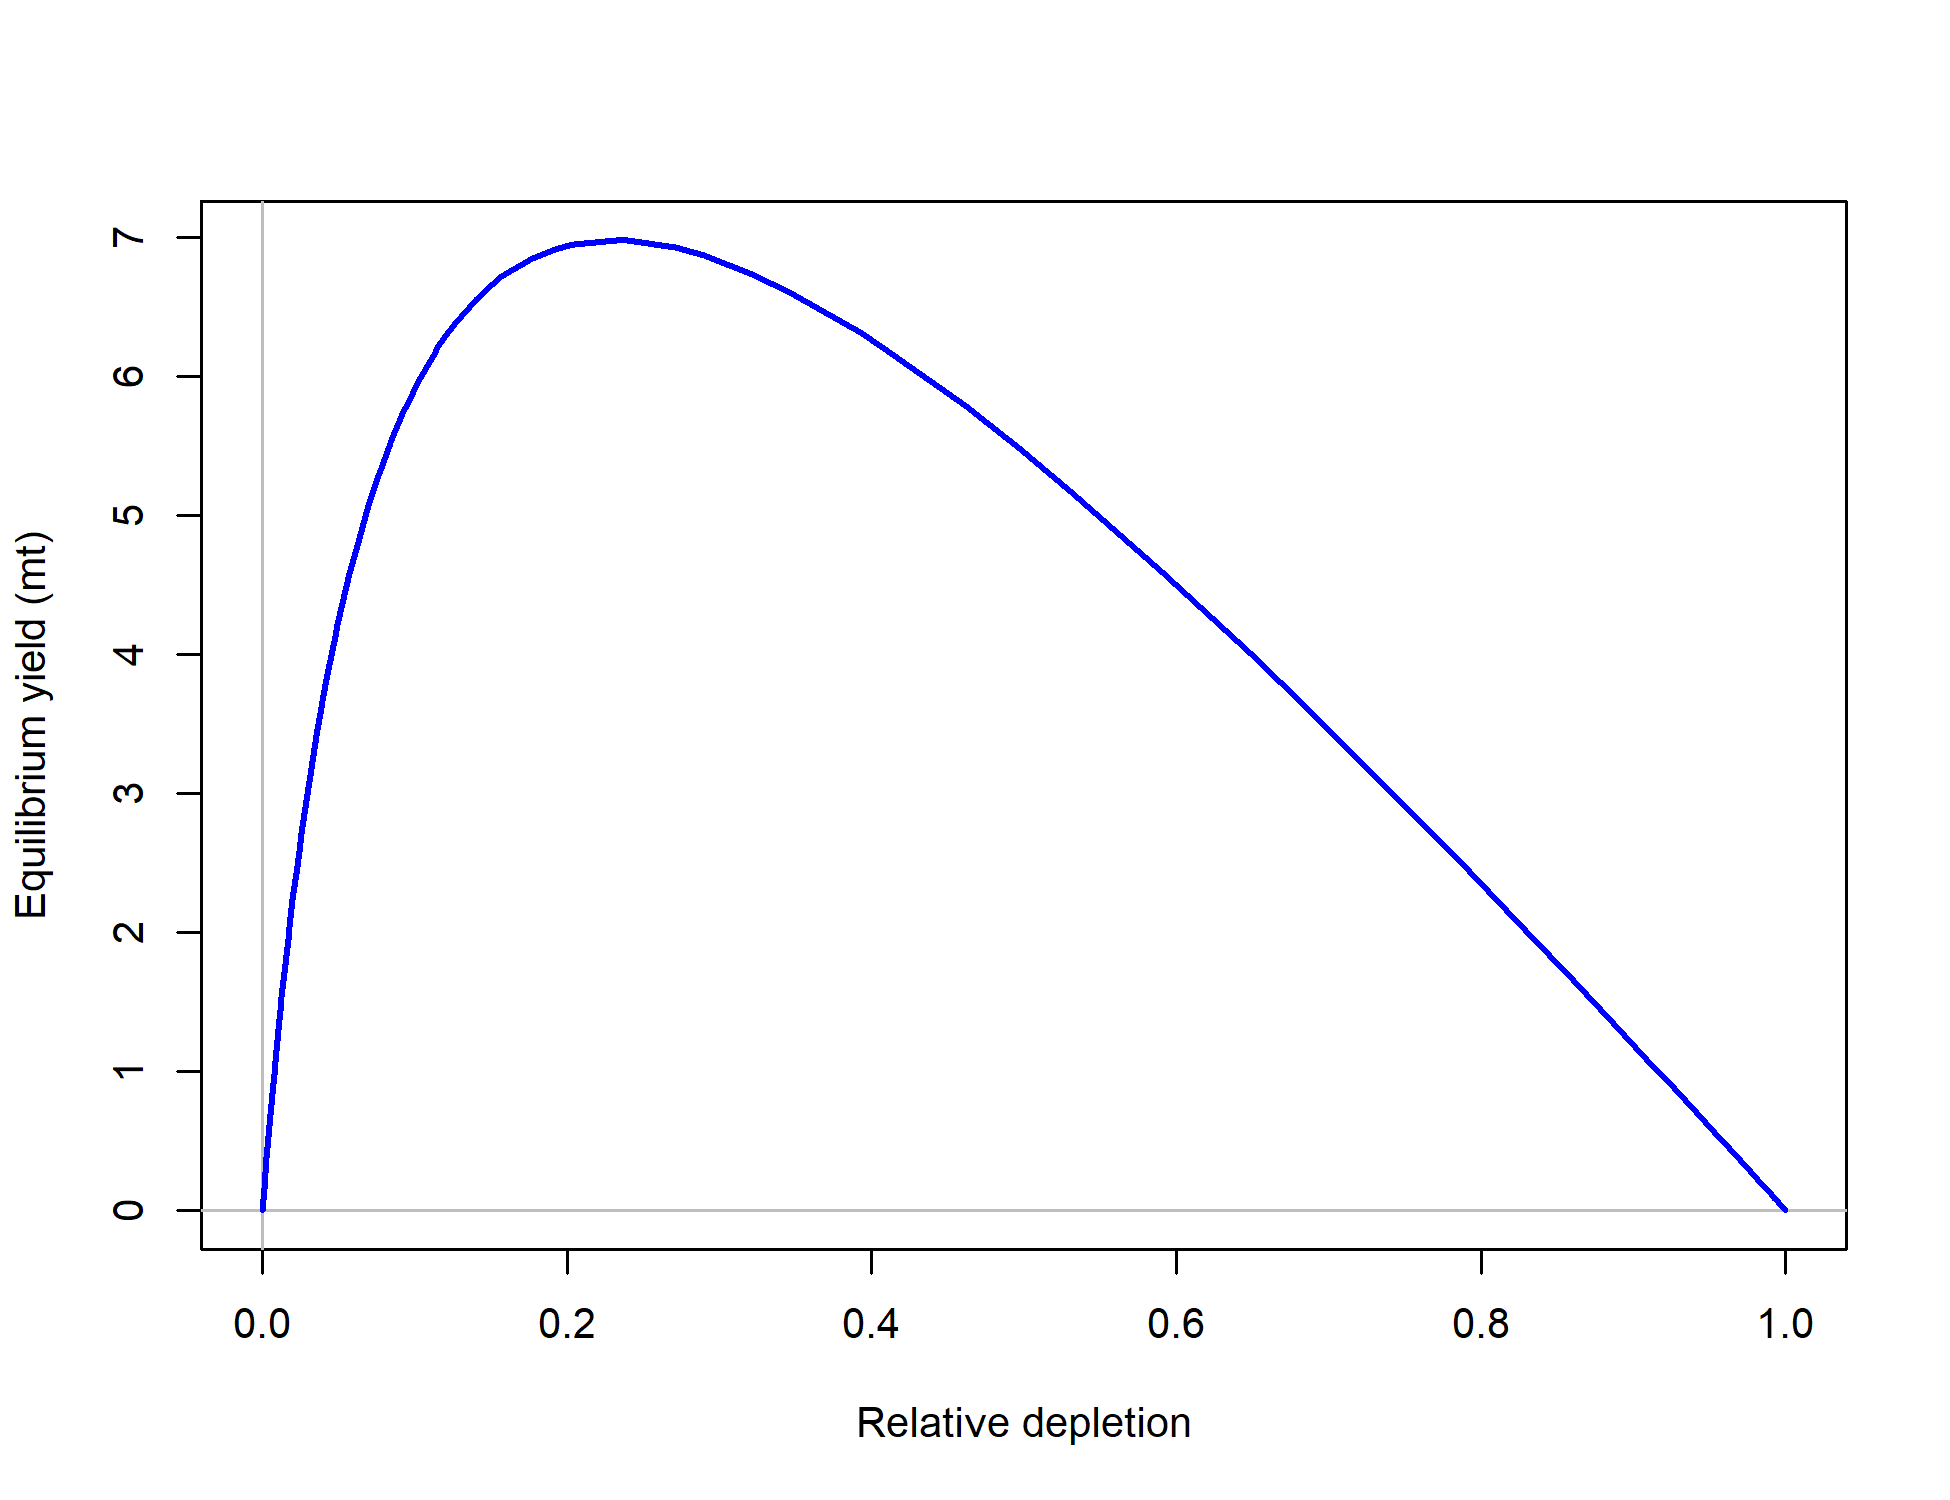
\includegraphics{r4ss/plots_mod1/yield1_yield_curve.png}
\caption{Equilibrium yield curve for the base case model. Values are
based on the 2014 fishery selectivity and with steepness fixed
at\ldots{} \label{fig:Yield_all}}
\end{figure}

\FloatBarrier

\newpage

\subsection*{Research And Data Needs}\label{research-and-data-needs}
\addcontentsline{toc}{subsection}{Research And Data Needs}

\hl{Include: identify information gaps that seriously impede the stock assessment.}

We recommend the following research be conducted before the next
assessment:

\begin{enumerate}

\item List item No. 1 in the list

\item List item No. 2 in the list, etc.

\end{enumerate}

\subsection*{Rebuilding Projections}\label{rebuilding-projections}
\addcontentsline{toc}{subsection}{Rebuilding Projections}

\hl{Include: reference to the principal results from rebuilding analysis if the 
stock is overfished. This section should be included in the Final/SAFE version 
assessment document but is not required for draft assessments undergoing review. 
See Rebuilding Analysis terms of reference for detailed information on 
rebuilding analysis requirements.}

\FloatBarrier

\newpage

\renewcommand{\thefigure}{\arabic{figure}}
\renewcommand{\thetable}{\arabic{table}}

\setcounter{figure}{0} \setcounter{table}{0}

\section{Introduction}\label{introduction}

\subsection{Basic Information}\label{basic-information}

\hl{Include: Scientific name, distribution, the basis of the choice of stock structure, 
including regional differences in life history or other biological characteristics 
that should form the basis of management units.}

\subsection{Map}\label{map}

A map showing the scope of the assessment and depicting boundaries for
fisheries or data collection strata is provided in Figure
\ref{fig:boundary_map}.

\subsection{Life History}\label{life-history}

\hl{Include: Important features of life history that affect management (e.g., migration, 
sexual dimorphism, bathymetric demography).}

\subsection{Ecosystem Considerations}\label{ecosystem-considerations-1}

\hl{Include: Ecosystem considerations (e.g., ecosystem role and trophic relationships of 
the species, habitat requirements/preferences, relevant data on ecosystem processes 
that may affect stock or parameters used in the stock assessment, and/or cross-FMP 
interactions with other fisheries). This section should note if environmental 
correlations or food web interactions were incorporated into the assessment model. 
The length and depth of this section would depend on availability of data and reports 
from the IEA, expertise of the STAT, and whether ecosystem factors are informational 
to contribute quantitative information to the assessment.}

\subsection{Fishery Information}\label{fishery-information}

\hl{Include: Important features of current fishery and relevant history of fishery.}

Rockfish example: The rockfish fishery off the U.S. Pacific coast first
developed off California in the late 19th century as a hook-and-line
fishery (Love et al. 2002).\\
The rockfish trawl fishery was established in the early 1940s, when the
United States became involved in World War II and wartime shortage of
red meat created an increased demand for other sources of protein (Harry
and Morgan 1961, Alverson et al. 1964). Etc\ldots{}.

\subsection{Summary of Management
History}\label{summary-of-management-history}

\hl{Include: Summary of management history (e.g., changes in mesh sizes, trip 
limits, or other management actions that may have significantly altered selection, 
catch rates, or discards).}

\subsection{Management Performance}\label{management-performance-1}

\hl{Include: Management performance, including a table or tables comparing 
Overfishing Limit (OFL), Annual Catch Limit (ACL), Harvest Guideline (HG) 
[CPS only], landings, and catch (i.e., landings plus discard) for each area and year.}

Management performance table: (Table \ref{tab:mnmgt_perform})\\
A summary of these values as well as other base case summary results can
be found in Table \ref{tab:base_summary}.

\subsection{Fisheries off Canada, Alaska, and/or
Mexico}\label{fisheries-off-canada-alaska-andor-mexico}

Include if necessary.

\section{Assessment}\label{assessment}

\subsection{Data}\label{data}

Data used in the China rockfish assessment are summarized in Figure
\ref{fig:data_plot}.\\
A description of each data source is below.

\subsubsection{Commercial Fishery
Landings}\label{commercial-fishery-landings}

\textbf{Sub-heading 1}

\textbf{Sub-heading 2}

\textbf{Sub-heading 3}

\subsubsection{Sport Fishery Removals}\label{sport-fishery-removals}

\textbf{Sub-heading 1}

\textbf{Sub-heading 2}

\textbf{Sub-heading 3}

\subsubsection{Estimated Discards}\label{estimated-discards}

\textbf{Sub-heading 1}

\textbf{Sub-heading 2}

\textbf{Sub-heading 3}

\subsubsection{Abundance Indices}\label{abundance-indices}

\textbf{Sub-heading 1}

\textbf{Sub-heading 2}

\subsubsection{Fishery-Independent Data: possible
sources}\label{fishery-independent-data-possible-sources}

\emph{Northwest Fisheries Science Center (NWFSC) slope survey}\\
The NWFSC slope survey was conducted annually from 1999 to 2002.\\
The depth range of this survey is 100-700 fm.

\emph{Northwest Fisheries Science Center (NWFSC) shelf-slope survey}\\
This survey is referred to as the ``combo,'' conducted annually since
2003.\\
The survey consistently covered depths between 30 and 700 fm.

\emph{Alaska Fisheries Science Center (AFSC) shelf survey}\\
The survey, often referred to as the ``triennial'' survey was conducted
every third year between 1977 and (and conducted in 2004 by the NWFSC
using the same protocols). The triennial survey trawls in depths of 30
to 275 fm.

\emph{Pikitch Study}\\
The Pikitch study was conducted between 1985 and 1987 (Pikitch et al.
1988). The northern and southern boundaries of the study were
\(48^\circ 42^\prime\) N latitude and \(42^\circ 60^\prime\) N. latitude
respectively, which is primarily within the Columbia INPFC area (Pikitch
et al. 1988 , Rogers and Pikitch 1992). Participation in the study was
voluntary and included vessels using bottom, midwater, and shrimp trawl
gears.\\
Observers of normal fishing operations on commercial vessels collected
the data, estimated the total weight of the catch by tow and recorded
the weight of species retained and discarded in the sample.

\emph{Enhanced Data Collection Project (EDCP)}\\
The EDCP was conducted by ODFW to collect information on bycatch and
discard groundfish species off the coast of Oregon from late 1995 to
early 1999.\\
EDCP had limited spatial coverage in Oregon waters only.

\emph{Partnership For Interdisciplinary Studies of Coastal Oceans
(PISCO)}\\
Blurb on species presence in PISCO surveys

\subsubsection{Biological Parameters and
Data}\label{biological-parameters-and-data}

\textbf{Length And Age Compositions}

Include: Sample size information for length and age composition data by
area, year, gear, market category, etc., including both the number of
trips and fish sampled.

Length compositions were provided from the following sources, by region,
with brief descriptions below:

\emph{Model 1}

\begin{itemize}[noitemsep,nolistsep,topsep=0pt]
  \item Source No. 1 (\emph{ex. research, commerical dead fish, live fish, etc},\\     
        date range (ex. 2010-2011)
  \item Source No. 2 (\emph{ex. research, commerical dead fish, live fish, etc},\\      
        date range (ex. 2010-2011) 
  \item etc...      
  \item Begin sublist if desired 
    \begin{itemize}[noitemsep,nolistsep]
      \item Sublist source No. 1     
      \item Sublist source No. 2        
      \item etc...     
    \end{itemize}
  \item Back to main list, next Source     
  \item Last Source     
\end{itemize}

Can duplicate this list if you have more than one assessment model

Possible sources of age and length data:

\emph{Recreational: Washington (WDFW)}

\emph{Recreational: California MRFSS And CRFS Length Composition Data}
Individual fish lengths recorded by MRFSS (1980-2003) and CRFS
(2004-2011) samplers were downloaded from the RecFIN website
(www.recfin.org). CRFS data from 2012-2014 were obtained directly from
CDFW.

\emph{Recreational: Oregon Recreational Boat Survey (ORBS)} Biological
data from the ORBS program were provided by ODFW. The ORBS is a dockside
sampling program for the both the recreational CPFV and private modes.
Length composition samples from north of Florence for the CPFV and
private fleets were provided from 1980-2014. Samples from south of
Florence spanned 1984-2014

\emph{Recreational: Miller and Gotshall (1965)}\\
The Northern California Marine Sport Fish Survey conducted an assessment
survey with goals that included estimation of annual fishing effort by
all recreational fishing modes, catch by weight, CPUE, and collection of
data to analyze length compositions

\emph{Commercial: PacFIN (Oregon and California)}

\emph{Research: NMFS Groundfish Ecology Survey}

From 2001-2005, the SWFSC Fisheries Ecology Division conducted longline
surveys aboard a chartered commercial longline vessel at various
stations between Monterey and Davenport, CA (\(36^\circ\) N. latitude to
\(37.5^\circ\) N. latitude) (pers. comm. Don Pearson, SWFSC). Longline
gear was set in various depths from 10 meters to 700 meters, parallel to
the depth contour. Each longline set consisted of 3-5 skates, each with
about 250 2/0 circle hooks baited with squid.\\
In nearshore habitats, the gear soaked for roughly 30 minutes.

\emph{Research: California Collaborative Fisheries Research Program
(CCFRP)}

\emph{Research: NWFSC shelf-slope survey}

\emph{Research: NWFSC slope survey}

\emph{Research: Abrams Thesis}

\vspace{.5cm}

\textbf{Age Structures}

Age structure data were available from the following sources:

\emph{Model Region 1}

\begin{itemize}[noitemsep,nolistsep,topsep=0pt]
  \item Source No. 1 (\emph{ex. research, commericla dead fish, live fish, etc},\\ 
        date range (ex. 2010-2011)
  \item Source No. 2 (\emph{ex. research, commericla dead fish, live fish, etc},\\
        date range (ex. 2010-2011) 
  \item etc...      
  \item Begin sublist if desired 
    \begin{itemize}[noitemsep,nolistsep]
      \item Sublist source No. 1     
      \item Sublist source No. 2        
      \item etc...     
    \end{itemize}
  \item Back to main list, next Source     
  \item Last Source     
\end{itemize}

Can duplicate this list if you have more than one assessment model

Length-at-age was initially estimated external to the population
dynamics models using the von Bertalanffy growth curve (Bertalanffy
1938), \(L_i = L_{\infty}e^{(-k[t-t_0])}\), where \(L_i\) is the length
(cm) at age \(i\), \(t\) is age in years, \(k\) is rate of increase in
growth, \(t_0\) is the intercept, and \(L_{\infty}\) is the asymptotic
length.

\vspace{.5cm}

\textbf{Aging Precision And Bias}

\vspace{.5cm}

\textbf{Weight-Length}

The weight-length relationship is based on the standard power function:
\(W = \alpha(L^\beta)\) where \(W\) is individual weight (kg), \(L\) is
length (cm), and \(\alpha\) and \(\beta\) are coefficients used as
constants.

\vspace{.5cm}

\textbf{Maturity And Fecundity}

\vspace{.5cm}

\textbf{Natural Mortality}

Natural mortality for wild fish populations is extremely difficult to
estimate.

\vspace{.5cm}

\textbf{Sex ratios}

\subsubsection{Environmental Or Ecosystem Data Included In The
Assessment}\label{environmental-or-ecosystem-data-included-in-the-assessment}

\subsection{History Of Modeling Approaches Used For This
Stock}\label{history-of-modeling-approaches-used-for-this-stock}

\subsubsection{Previous Assessments}\label{previous-assessments}

\subsubsection{Previous Assessment
Recommendations}\label{previous-assessment-recommendations}

Include: Response to STAR panel recommendations from the most recent
previous assessment.

\begin{description}[style=unboxed]

  \item[Recommendation 1: blah blah blah.] \hfill \\

   STAT response: blah blah blah....

\item[Recommendation 2: blah blah blah.] \hfill \\

  STAT response: blah blah blah....

\item[Recommendation 3: blah blah blah., etc.] \hfill \\

  STAT response: Continue recommendations as needed


\end{description}

\subsection{Model Description}\label{model-description}

\subsubsection{Transition To The Current Stock
Assessment}\label{transition-to-the-current-stock-assessment}

Include: Complete description of any new modeling approaches

Below, we describe the most important changes made since the last full
assessment and explain rationale for each change.:

\begin{enumerate}
\def\labelenumi{\arabic{enumi}.}
\item
  Change No. 1. \emph{Rationale}: blah blah blah.
\item
  Change No. 2. \emph{Rationale}: blah blah blah.
\item
  Change No. 3. \emph{Rationale}: Continue list as needed.
\end{enumerate}

\subsubsection{Definition of Fleets and
Areas}\label{definition-of-fleets-and-areas}

We generated data sources for each of the models. Fleets by model
include:

\textbf{Model Region 1 or remove this line if only one model}

\emph{Commercial}: The commercial fleets include\ldots{}

\emph{Recreational}: The recreational fleets include\ldots{}

\emph{Research}: Research derived-data include\ldots{}

\subsubsection{Summary of Data for Fleets and
Areas}\label{summary-of-data-for-fleets-and-areas}

\subsubsection{Modeling Software}\label{modeling-software}

The STAT team used Stock Synthesis 3 version 3.24u by Dr.~Richard Methot
at the NWFSC. This most recent version (SS-V3.24u) was used, since it
included improvements and corrections to older versions.

\subsubsection{Data Weighting}\label{data-weighting}

Citation for Francis method (Francis 2011)\\
Citation for Ianelli-McAllister harmonic mean method (McAllister and
Ianelli 1997)

\subsubsection{Priors}\label{priors}

Citation for Hamel prior on natural mortality (Hamel 2015)

\subsubsection{General Model
Specifications}\label{general-model-specifications}

Citation for posterior predictive fecundity relationship from Dick
(2009)\\
Model data, control, starter, and forecast files can be found in
Appendices A-D.

\subsubsection{Estimated And Fixed
Parameters}\label{estimated-and-fixed-parameters}

A full list of all estimated and fixed parameters is provided in
Tables\ldots{}. Estimated and fixed parameters tables currently read in
from .csv file, EXAMPLE: Table \ref{tab:Model1_params}

\subsection{Model Selection and
Evaluation}\label{model-selection-and-evaluation}

\subsubsection{Key Assumptions and Structural
Choices}\label{key-assumptions-and-structural-choices}

Include: Evidence of search for balance between model realism and
parsimony.\\
Comparison of key model assumptions, include comparisons based on nested
models (e.g., asymptotic vs.~domed selectivities, constant
vs.~time-varying selectivities).

\subsubsection{Alternate Models
Considered}\label{alternate-models-considered}

Include: Summary of alternate model configurations that were tried but
rejected.

\subsubsection{Convergence}\label{convergence}

Include: Randomization run results or other evidence of search for
global best estimates.

Convergence testing through use of dispersed starting values often
requires extreme values to actually explore new areas of the
multivariate likelihood surface. Jitter is a SS option that generates
random starting values from a normal distribution logistically
transformed into each parameter's range (Methot 2015). Table
\ref{tab:jitter} shows the results of running 100 jitters for each
pre-STAR base model\ldots{}.

\subsection{Response To The Current STAR Panel
Requests}\label{response-to-the-current-star-panel-requests}

\begin{description}[style=unboxed]

\item[Request No. 1: Add after STAR panel.] \hfill \\

    \textbf{Rationale:} Add after STAR panel.  

    \textbf{STAT Response:} Add after STAR panel.

\item[Request No. 2: Add after STAR panel.] \hfill \\

    \textbf{Rationale:} Add after STAR panel.

    \textbf{STAT Response:} Add after STAR panel.

\item[Request No. 3: Add after STAR panel.] \hfill \\

    \textbf{Rationale:} Add after STAR panel.
  
    \textbf{STAT Response:} Add after STAR panel.

\item[Request No. 4: Example of a request that may have a list:] \hfill \\
\begin{itemize}
\item \textbf{Item No. 1}
\item \textbf{Item No. 2}
\item \textbf{Item No. 3, etc.}
\end{itemize}

    \textbf{Rationale:} Add after STAR panel.

    \textbf{STAT Response:} Continue requests as needed.


\end{description}

\subsection{Model 1}\label{model-1}

\subsubsection{Model 1 Base Case
Results}\label{model-1-base-case-results}

Table \ref{tab:Model1_params}

\subsubsection{Model 1 Uncertainty and Sensitivity
Analyses}\label{model-1-uncertainty-and-sensitivity-analyses}

Table \ref{tab:Sensitivity_model1}

\subsubsection{Model 1 Retrospective
Analysis}\label{model-1-retrospective-analysis}

\subsubsection{Model 1 Likelihood
Profiles}\label{model-1-likelihood-profiles}

\subsubsection{Model 1 Harvest Control Rules (CPS
only)}\label{model-1-harvest-control-rules-cps-only}

\subsubsection{Model 1 Reference Points (groundfish
only)}\label{model-1-reference-points-groundfish-only}

Intro sentence or two\ldots{}.(Table \ref{tab:Timeseries_mod1}).

Equilibrium yield at the proxy \(F_{MSY}\) harvest rate corresponding to
\(SPR_{50\%}\) is 5.8 mt. Table \ref{tab:Ref_pts_mod1} shows the full
suite of estimated reference points for the northern area model and
Figure \ref{fig:Yield_all} shows the equilibrium yield curve.

\subsection{Model 2}\label{model-2}

\subsubsection{Model 2 Base Case
Results}\label{model-2-base-case-results}

\subsubsection{Model 2 Uncertainty and Sensitivity
Analyses}\label{model-2-uncertainty-and-sensitivity-analyses}

\subsubsection{Model 2 Retrospective
Analysis}\label{model-2-retrospective-analysis}

\subsubsection{Model 2 Likelihood
Profiles}\label{model-2-likelihood-profiles}

\subsubsection{Model 2 Harvest Control Rules (CPS
only)}\label{model-2-harvest-control-rules-cps-only}

\subsubsection{Model 2 Reference Points (groundfish
only)}\label{model-2-reference-points-groundfish-only}

\subsection{Model 3}\label{model-3}

\subsubsection{Model 3 Base Case
Results}\label{model-3-base-case-results}

\subsubsection{Model 3 Uncertainty and Sensitivity
Analyses}\label{model-3-uncertainty-and-sensitivity-analyses}

\subsubsection{Model 3 Retrospective
Analysis}\label{model-3-retrospective-analysis}

\subsubsection{Model 3 Likelihood
profiles}\label{model-3-likelihood-profiles}

\subsubsection{Model 3 Harvest Control Rules (CPS
only)}\label{model-3-harvest-control-rules-cps-only}

\subsubsection{Model 3 Reference Points (groundfish
only)}\label{model-3-reference-points-groundfish-only}

\section{Harvest Projections and Decision
Tables}\label{harvest-projections-and-decision-tables}

Table \ref{tab:mnmgt_perform}

\textbf{Model 1 Projections and Decision Table (groundfish only)} (Table
\ref{tab:Forecast_mod1}

Table \ref{tab:Decision_table_mod1}

\textbf{Model 2 Projections and Decision Table (groundfish only)}

\textbf{Model 3 Projections and Decision Table (groundfish only)}

\section{Regional Management
Considerations}\label{regional-management-considerations}

\begin{enumerate}
\def\labelenumi{\arabic{enumi}.}
\tightlist
\item
  For stocks where current practice is to allocate harvests by
  management area, a recommended method of allocating harvests based on
  the distribution of biomass should be provided. The MT advisor should
  be consulted on the appropriate management areas for each stock.
\item
  Discuss whether a regional management approach makes sense for the
  species from a biological perspective.
\item
  If there are insufficient data to analyze a regional management
  approach, what are the research and data needs to answer this
  question?
\end{enumerate}

\section{Research Needs}\label{research-needs}

\begin{enumerate}

\item Research need No. 1

\item Research need No. 2

\item Research need No. 3

\item etc.

\end{enumerate}

\section{Acknowledgments}\label{acknowledgments}

Include: STAR panel members and affiliations as well as names and
affiliations of persons who contributed data, advice or information but
were not part of the assessment team. Not required in draft assessment
undergoing review.

\newpage

\FloatBarrier

\section{Tables}\label{tables}

\FloatBarrier

\FloatBarrier

\begin{landscape}
\begin{longtable}{rlrrcrcl}
\caption{List of parameters used in
                                              the base model, including estimated 
                                              values and standard deviations (SD), 
                                              bounds (minimum and maximum), 
                                              estimation phase (negative values indicate
                                              not estimated), status (indicates if 
                                              parameters are near bounds, and prior type
                                              information (mean, SD).} \\ 
  \hline
No. & Parameter & Value & SD & Bounds & Phase & Status & Prior \\ 
  \hline 
\endhead 
\hline 
\multicolumn{3}{l}{\footnotesize Continued on next page} 
\endfoot 
\endlastfoot 
 \hline
1 & NatM\_p\_1\_Fem\_GP\_1 & 0.07 &  & (0.01, 0.15) & -3 &  & Log\_Norm (-2.94, 0.53) \\ 
  2 & L\_at\_Amin\_Fem\_GP\_1 & 2.00 &  & (-10, 45) & -2 &  & Normal (2, 10) \\ 
  3 & L\_at\_Amax\_Fem\_GP\_1 & 35.41 & 0.36 & (20, 50) & 6 & OK & Normal (34, 10) \\ 
  4 & VonBert\_K\_Fem\_GP\_1 & 0.15 & 0.01 & (0.01, 0.3) & 6 & OK & Normal (0.1, 0.8) \\ 
  5 & CV\_young\_Fem\_GP\_1 & 0.10 &  & (0.01, 0.25) & -6 &  & None \\ 
  6 & CV\_old\_Fem\_GP\_1 & 0.08 & 0.01 & (0.01, 0.25) & 6 & OK & None \\ 
  7 & NatM\_p\_1\_Mal\_GP\_1 & 0.00 &  & (-1, 0.15) & -3 &  & None \\ 
  8 & L\_at\_Amin\_Mal\_GP\_1 & 0.00 &  & (-1, 45) & -2 &  & Normal (2, 10) \\ 
  9 & L\_at\_Amax\_Mal\_GP\_1 & 0.00 &  & (-1, 50) & -4 &  & Normal (33.13, 10) \\ 
  10 & VonBert\_K\_Mal\_GP\_1 & 0.00 &  & (-1, 0.3) & -4 &  & Normal (0.246, 0.8) \\ 
  11 & CV\_young\_Mal\_GP\_1 & 0.00 &  & (-1, 0.25) & -3 &  & None \\ 
  12 & CV\_old\_Mal\_GP\_1 & 0.00 &  & (-1, 0.25) & -3 &  & None \\ 
  13 & Wtlen\_1\_Fem & 0.00 &  & (0, 1) & -3 &  & None \\ 
  14 & Wtlen\_2\_Fem & 3.18 &  & (2, 4) & -3 &  & None \\ 
  15 & Mat50\%\_Fem & 28.50 &  & (1, 100) & -3 &  & None \\ 
  16 & Mat\_slope\_Fem & -1.00 &  & (-9, 9) & -3 &  & None \\ 
  17 & Eggs/kg\_inter\_Fem & 0.20 &  & (-3, 3) & -3 &  & None \\ 
  18 & Eggs/kg\_slope\_wt\_Fem & 0.06 &  & (-3, 3) & -3 &  & None \\ 
  19 & Wtlen\_1\_Mal & 0.00 &  & (0, 1) & -3 &  & None \\ 
  20 & Wtlen\_2\_Mal & 3.18 &  & (2, 4) & -3 &  & None \\ 
  24 & CohortGrowDev & 0.00 &  & (0, 0) & -4 &  & None \\ 
  25 & SR\_LN(R0) & 3.53 & 0.18 & (2, 12) & 1 & OK & None \\ 
  26 & SR\_BH\_steep & 0.77 &  & (0.2, 1) & -3 &  & Full\_Beta (0.773, 0.147) \\ 
  27 & SR\_sigmaR & 0.50 &  & (0, 2) & -3 &  & None \\ 
  28 & SR\_envlink & 0.10 &  & (-5, 5) & -3 &  & None \\ 
  29 & SR\_R1\_offset & 0.00 &  & (-5, 5) & -4 &  & None \\ 
  30 & SR\_autocorr & 0.00 &  & (0, 0) & -99 &  & None \\ 
  68 & InitF\_11\_WA\_SouthernWA\_Rec\_PCPR & 0.00 &  & (0, 1) & -1 &  & None \\ 
  69 & InitF\_22\_WA\_NorthernWA\_Rec\_PC & 0.00 &  & (0, 1) & -1 &  & None \\ 
  70 & InitF\_33\_WA\_NorthernWA\_Rec\_PR & 0.00 &  & (0, 1) & -1 &  & None \\ 
  71 & Q\_extraSD\_3\_3\_WA\_NorthernWA\_Rec\_PR & 0.13 & 0.02 & (0, 2) & 2 & OK & None \\ 
  72 & SizeSel\_1P\_1\_1\_WA\_SouthernWA\_Rec\_PCPR & 34.89 &  & (19, 36) & -4 &  & None \\ 
  73 & SizeSel\_1P\_2\_1\_WA\_SouthernWA\_Rec\_PCPR & -4.00 &  & (-9, 5) & -9 &  & None \\ 
  74 & SizeSel\_1P\_3\_1\_WA\_SouthernWA\_Rec\_PCPR & 3.97 & 0.36 & (0, 9) & 5 & OK & None \\ 
  75 & SizeSel\_1P\_4\_1\_WA\_SouthernWA\_Rec\_PCPR & 8.00 &  & (0, 9) & -9 &  & None \\ 
  76 & SizeSel\_1P\_5\_1\_WA\_SouthernWA\_Rec\_PCPR & -8.00 &  & (-9, 9) & -9 &  & None \\ 
  77 & SizeSel\_1P\_6\_1\_WA\_SouthernWA\_Rec\_PCPR & 8.00 &  & (-9, 9) & -9 &  & None \\ 
  78 & SizeSel\_2P\_1\_2\_WA\_NorthernWA\_Rec\_PC & 34.86 & 1.00 & (19, 36) & 4 & OK & None \\ 
  79 & SizeSel\_2P\_2\_2\_WA\_NorthernWA\_Rec\_PC & -4.00 &  & (-9, 5) & -9 &  & None \\ 
  80 & SizeSel\_2P\_3\_2\_WA\_NorthernWA\_Rec\_PC & 2.92 & 0.35 & (0, 9) & 5 & OK & None \\ 
  81 & SizeSel\_2P\_4\_2\_WA\_NorthernWA\_Rec\_PC & 8.00 &  & (0, 9) & -9 &  & None \\ 
  82 & SizeSel\_2P\_5\_2\_WA\_NorthernWA\_Rec\_PC & -8.00 &  & (-9, 9) & -9 &  & None \\ 
  83 & SizeSel\_2P\_6\_2\_WA\_NorthernWA\_Rec\_PC & 8.00 &  & (-9, 9) & -9 &  & None \\ 
   \hline
\hline
\label{tab:model_params}
\end{longtable}
\end{landscape}

\newpage

\begin{table}[ht]
\centering
\caption{Summary of the biomass/abundance
                                              time series used in the stock
                                              assessment.} 
\label{tab:Index_summary}
\begin{tabular}{>{\centering}p{.4in}>{\centering}p{.3in}>{\centering}p{.3in}>{\centering}p{.3in}>{\centering}p{.6in}>{\centering}p{.5in}>{\centering}p{.8in}>{\centering}p{.8in}>{\centering}p{.3in}>{\centering}p{.5in}}
  \hline
Region & ID & Fleet & Years & Name & Fishery ind. & Filtering & Method & Rank & Endorsed \\ 
  \hline
WA & 1 & 4 & 1981-2014 & Dockside CPUE & No & trip, area, month, Stephens-MacCall & delta-GLM (bin-gamma) & 1 & SSC \\ 
  - & - & - & - & - & - & - & - & - & - \\ 
  - & - & - & - & - & - & - & - & - & - \\ 
  - & - & - & - & - & - & - & - & - & - \\ 
   \hline
\end{tabular}
\end{table}

\newpage

\begin{table}[ht]
\centering
\caption{Results from 100 jitters from each of 
                                      the three models.} 
\label{tab:jitter}
\begin{tabular}{llll}
  \hline
Status & Model.1 & Model.2 & Model.3 \\ 
  \hline
Returned to base case & - & - & - \\ 
  Found local minimum & - & - & - \\ 
  Found better solution & - & - & - \\ 
  Error in likelihood & - & - & - \\ 
  Total & 100 & 100 & 100 \\ 
   \hline
\end{tabular}
\end{table}

\FloatBarrier

\newpage

\begin{sidewaystable}[ht]
\centering
\caption{Sensitivity of the base model 
                                          to dropping or down-weighting data 
                                          sources and alternative assumptions 
                                          about growth.} 
\label{tab:Sensitivity_model1}
\scalebox{0.9}{
\begin{tabular}{l>{\centering}p{.6in}>{\centering}p{.6in}>{\centering}p{.6in}>{\centering}p{.6in}>{\centering}p{.6in}>{\centering}p{.6in}>{\centering}p{.6in}>{\centering}p{.6in}}
  \hline
Label & Base (Francis weights) & Harmonic mean weights & Drop index & Drop ages & Down-weight lengths & Free size Age0 & Free CV Amin & External growth \\ 
  \hline
TOTAL\_like & - & - & - & - & - & - & - & - \\ 
  Catch\_like & - & - & - & - & - & - & - & - \\ 
  Equil\_catch\_like & - & - & - & - & - & - & - & - \\ 
  Survey\_like & - & - & - & - & - & - & - & - \\ 
  Length\_comp\_like & - & - & - & - & - & - & - & - \\ 
  Age\_comp\_like & - & - & - & - & - & - & - & - \\ 
  Parm\_priors\_like & - & - & - & - & - & - & - & - \\ 
  SSB\_Unfished\_thousand\_mt & - & - & - & - & - & - & - & - \\ 
  TotBio\_Unfished & - & - & - & - & - & - & - & - \\ 
  SmryBio\_Unfished & - & - & - & - & - & - & - & - \\ 
  Recr\_Unfished\_billions & - & - & - & - & - & - & - & - \\ 
  SSB\_Btgt\_thousand\_mt & - & - & - & - & - & - & - & - \\ 
  SPR\_Btgt & - & - & - & - & - & - & - & - \\ 
  Fstd\_Btgt & - & - & - & - & - & - & - & - \\ 
  TotYield\_Btgt\_thousand\_mt & - & - & - & - & - & - & - & - \\ 
  SSB\_SPRtgt\_thousand\_mt & - & - & - & - & - & - & - & - \\ 
  Fstd\_SPRtgt & - & - & - & - & - & - & - & - \\ 
  TotYield\_SPRtgt\_thousand\_mt & - & - & - & - & - & - & - & - \\ 
  SSB\_MSY\_thousand\_mt & - & - & - & - & - & - & - & - \\ 
  SPR\_MSY & - & - & - & - & - & - & - & - \\ 
  Fstd\_MSY & - & - & - & - & - & - & - & - \\ 
  TotYield\_MSY\_thousand\_mt & - & - & - & - & - & - & - & - \\ 
  RetYield\_MSY & - & - & - & - & - & - & - & - \\ 
  Bratio\_2015 & - & - & - & - & - & - & - & - \\ 
  F\_2015 & - & - & - & - & - & - & - & - \\ 
  SPRratio\_2015 & - & - & - & - & - & - & - & - \\ 
  Recr\_2015 & - & - & - & - & - & - & - & - \\ 
  Recr\_Virgin\_billions & - & - & - & - & - & - & - & - \\ 
  L\_at\_Amin\_Fem\_GP\_1 & - & - & - & - & - & - & - & - \\ 
  L\_at\_Amax\_Fem\_GP\_1 & - & - & - & - & - & - & - & - \\ 
  VonBert\_K\_Fem\_GP\_1 & - & - & - & - & - & - & - & - \\ 
  CV\_young\_Fem\_GP\_1 & - & - & - & - & - & - & - & - \\ 
  CV\_old\_Fem\_GP\_1 & - & - & - & - & - & - & - & - \\ 
   \hline
\end{tabular}
}
\end{sidewaystable}

\newpage

\begin{longtable}{c>{\centering}p{.6in}>{\centering}p{.6in}>{\centering}p{.6in}>{\centering}p{.6in}>{\centering}p{.8in}>{\centering}p{.8in}c}
\caption{Time-series of population estimates 
                                        from the base-case model.} \\ 
  \hline
Year & Total biomass (mt) & Spawning biomass (mt) & Depletion & Age-0 recruits & Total catch (mt) & Relative exploitation rate & SPR \\ 
  \hline \endhead  \hline
1900 & 240.806 & 2.44e+01 & 0 & 34.1631 & 0 & 0 & 1 \\ 
  1901 & 240.806 & 2.44e+01 & 0 & 34.1631 & 0 & 0 & 1 \\ 
  1902 & 240.806 & 2.44e+01 & 0 & 34.1631 & 0 & 0 & 1 \\ 
  1903 & 240.806 & 2.44e+01 & 0 & 34.1631 & 0 & 0 & 1 \\ 
  1904 & 240.806 & 2.44e+01 & 0 & 34.1631 & 0 & 0 & 1 \\ 
  1905 & 240.806 & 2.44e+01 & 0 & 34.1631 & 0 & 0 & 1 \\ 
  1906 & 240.806 & 2.44e+01 & 0 & 34.1631 & 0 & 0 & 1 \\ 
  1907 & 240.806 & 2.44e+01 & 0 & 34.1631 & 0 & 0 & 1 \\ 
  1908 & 240.806 & 2.44e+01 & 0 & 34.1631 & 0 & 0 & 1 \\ 
  1909 & 240.806 & 2.44e+01 & 0 & 34.1631 & 0 & 0 & 1 \\ 
  1910 & 240.806 & 2.44e+01 & 0 & 34.1631 & 0 & 0 & 1 \\ 
  1911 & 240.806 & 2.44e+01 & 0 & 34.1632 & 0 & 0 & 1 \\ 
  1912 & 240.806 & 2.44e+01 & 0 & 34.1632 & 0 & 0 & 1 \\ 
  1913 & 240.806 & 2.44e+01 & 0 & 34.1632 & 0 & 0 & 1 \\ 
  1914 & 240.806 & 2.44e+01 & 0 & 34.1632 & 0 & 0 & 1 \\ 
  1915 & 240.806 & 2.44e+01 & 0 & 34.1633 & 0 & 0 & 1 \\ 
  1916 & 240.806 & 2.44e+01 & 0 & 34.1633 & 0 & 0 & 1 \\ 
  1917 & 240.806 & 2.44e+01 & 0 & 34.1633 & 0 & 0 & 1 \\ 
  1918 & 240.806 & 2.44e+01 & 0 & 34.1633 & 0 & 0 & 1 \\ 
  1919 & 240.806 & 2.44e+01 & 0 & 34.1634 & 0 & 0 & 1 \\ 
  1920 & 240.806 & 2.44e+01 & 0 & 34.1634 & 0 & 0 & 1 \\ 
  1921 & 240.806 & 2.44e+01 & 0 & 34.1634 & 0 & 0 & 1 \\ 
  1922 & 240.806 & 2.44e+01 & 0 & 34.1635 & 0 & 0 & 1 \\ 
  1923 & 240.806 & 2.44e+01 & 0 & 34.1635 & 0 & 0 & 1 \\ 
  1924 & 240.806 & 2.44e+01 & 0 & 34.1635 & 0 & 0 & 1 \\ 
  1925 & 240.806 & 2.44e+01 & 0 & 34.1635 & 0 & 0 & 1 \\ 
  1926 & 240.806 & 2.44e+01 & 0 & 34.1635 & 0 & 0 & 1 \\ 
  1927 & 240.806 & 2.44e+01 & 0 & 34.1636 & 0 & 0 & 1 \\ 
  1928 & 240.806 & 2.44e+01 & 0 & 34.1636 & 0 & 0 & 1 \\ 
  1929 & 240.806 & 2.44e+01 & 0 & 34.1636 & 0 & 0 & 1 \\ 
  1930 & 240.806 & 2.44e+01 & 0 & 34.1636 & 0 & 0 & 1 \\ 
  1931 & 240.806 & 2.44e+01 & 0 & 34.1636 & 0 & 0 & 1 \\ 
  1932 & 240.806 & 2.44e+01 & 0 & 34.1637 & 0 & 0 & 1 \\ 
  1933 & 240.806 & 2.44e+01 & 0 & 34.1637 & 0 & 0 & 1 \\ 
  1934 & 240.806 & 2.44e+01 & 0 & 34.1637 & 0 & 0 & 1 \\ 
  1935 & 240.806 & 2.44e+01 & 0 & 34.1637 & 0 & 0 & 1 \\ 
  1936 & 240.806 & 2.44e+01 & 0 & 34.1637 & 0 & 0 & 1 \\ 
  1937 & 240.806 & 2.44e+01 & 0 & 34.1637 & 0 & 0 & 1 \\ 
  1938 & 240.806 & 2.44e+01 & 0 & 34.1637 & 0 & 0 & 1 \\ 
  1939 & 240.806 & 2.44e+01 & 0 & 34.1637 & 0 & 0 & 1 \\ 
  1940 & 240.806 & 2.44e+01 & 0 & 34.1637 & 0 & 0 & 1 \\ 
  1941 & 240.806 & 2.44e+01 & 0 & 34.1638 & 0 & 0 & 1 \\ 
  1942 & 240.806 & 2.44e+01 & 0 & 34.1638 & 0 & 0 & 1 \\ 
  1943 & 240.806 & 2.44e+01 & 0 & 34.1638 & 0 & 0 & 1 \\ 
  1944 & 240.806 & 2.44e+01 & 0 & 34.1638 & 0 & 0 & 1 \\ 
  1945 & 240.806 & 2.44e+01 & 0 & 34.1638 & 0 & 0 & 1 \\ 
  1946 & 240.806 & 2.44e+01 & 0 & 34.1638 & 0 & 0 & 1 \\ 
  1947 & 240.806 & 2.44e+01 & 0 & 34.1638 & 0 & 0 & 1 \\ 
  1948 & 240.806 & 2.44e+01 & 0 & 34.1638 & 0 & 0 & 1 \\ 
  1949 & 240.806 & 2.44e+01 & 0 & 34.1638 & 0 & 0 & 1 \\ 
  1950 & 240.806 & 2.44e+01 & 0 & 34.1638 & 0 & 0 & 1 \\ 
  1951 & 240.806 & 2.44e+01 & 0 & 34.1638 & 0 & 0 & 1 \\ 
  1952 & 240.806 & 2.44e+01 & 0 & 34.1638 & 0 & 0 & 1 \\ 
  1953 & 240.806 & 2.44e+01 & 0 & 34.1638 & 0 & 0 & 1 \\ 
  1954 & 240.806 & 2.44e+01 & 0 & 34.1638 & 0 & 0 & 1 \\ 
  1955 & 240.806 & 2.44e+01 & 0 & 34.1638 & 0 & 0 & 1 \\ 
  1956 & 240.806 & 2.44e+01 & 0 & 34.1638 & 0 & 0 & 1 \\ 
  1957 & 240.806 & 2.44e+01 & 0 & 34.1638 & 0 & 0 & 1 \\ 
  1958 & 240.806 & 2.44e+01 & 0 & 34.1639 & 0 & 0 & 1 \\ 
  1959 & 240.806 & 2.44e+01 & 0 & 34.1639 & 0 & 0 & 1 \\ 
  1960 & 240.806 & 2.44e+01 & 0 & 34.1639 & 0 & 0 & 1 \\ 
  1961 & 240.806 & 2.44e+01 & 0 & 34.1639 & 0 & 0 & 1 \\ 
  1962 & 240.806 & 2.44e+01 & 0 & 34.1639 & 0 & 0 & 1 \\ 
  1963 & 240.806 & 2.44e+01 & 0 & 34.1639 & 0 & 0 & 1 \\ 
  1964 & 240.806 & 2.44e+01 & 0 & 34.1639 & 0 & 0 & 1 \\ 
  1965 & 240.806 & 2.44e+01 & 0 & 34.1639 & 0 & 0 & 1 \\ 
  1966 & 240.806 & 2.44e+01 & 0 & 34.1639 & 0 & 0 & 1 \\ 
  1967 & 223.102 & 2.44e+01 & 0 & 34.1639 & 1.31 & 0 & 0.91 \\ 
  1968 & 219.589 & 2.43e+01 & 0.99 & 34.1491 & 1.59 & 0 & 0.89 \\ 
  1969 & 216.262 & 2.41e+01 & 0.99 & 34.1316 & 1.86 & 0.17 & 0.87 \\ 
  1970 & 212.766 & 2.39e+01 & 0.98 & 34.1115 & 2.15 & 0.2 & 0.86 \\ 
  1971 & 209.434 & 2.37e+01 & 0.97 & 34.0886 & 2.43 & 0.23 & 0.84 \\ 
  1972 & 206.144 & 2.35e+01 & 0.96 & 34.063 & 2.71 & 0.26 & 0.82 \\ 
  1973 & 202.901 & 2.32e+01 & 0.95 & 34.0348 & 2.99 & 0.29 & 0.8 \\ 
  1974 & 199.776 & 2.30e+01 & 0.94 & 34.004 & 3.26 & 0.32 & 0.79 \\ 
  1975 & 196.575 & 2.27e+01 & 0.93 & 33.9706 & 3.54 & 0.35 & 0.77 \\ 
  1976 & 214.297 & 2.24e+01 & 0.92 & 33.9346 & 1.88 & 0.19 & 0.86 \\ 
  1977 & 220.007 & 2.23e+01 & 0.91 & 33.9217 & 1.42 & 0.14 & 0.89 \\ 
  1978 & 192.863 & 2.22e+01 & 0.91 & 33.9158 & 3.86 & 0.39 & 0.75 \\ 
  1979 & 200.664 & 2.19e+01 & 0.9 & 33.8778 & 3.03 & 0.31 & 0.79 \\ 
  1980 & 205.144 & 2.17e+01 & 0.89 & 33.8522 & 2.59 & 0.27 & 0.82 \\ 
  1981 & 207.538 & 2.16e+01 & 0.88 & 33.8337 & 2.36 & 0.24 & 0.83 \\ 
  1982 & 202.508 & 2.14e+01 & 0.88 & 33.8195 & 2.79 & 0.29 & 0.8 \\ 
  1983 & 199.611 & 2.13e+01 & 0.87 & 33.7998 & 3.04 & 0.32 & 0.79 \\ 
  1984 & 195.443 & 2.11e+01 & 0.86 & 33.7774 & 3.4 & 0.36 & 0.77 \\ 
  1985 & 195.356 & 2.09e+01 & 0.86 & 33.7506 & 3.38 & 0.36 & 0.77 \\ 
  1986 & 189.136 & 2.07e+01 & 0.85 & 33.725 & 3.96 & 0.42 & 0.73 \\ 
  1987 & 179.585 & 2.05e+01 & 0.84 & 33.6914 & 4.96 & 0.53 & 0.69 \\ 
  1988 & 170.707 & 2.02e+01 & 0.82 & 33.643 & 5.96999 & 0.65 & 0.64 \\ 
  1989 & 162.489 & 1.97e+01 & 0.81 & 33.5791 & 6.96999 & 0.77 & 0.6 \\ 
  1990 & 154.635 & 1.92e+01 & 0.79 & 33.4985 & 7.97999 & 0.9 & 0.56 \\ 
  1991 & 181.084 & 1.86e+01 & 0.76 & 33.3996 & 4.32 & 0.5 & 0.69 \\ 
  1992 & 154.687 & 1.84e+01 & 0.75 & 33.3684 & 7.61999 & 0.89 & 0.56 \\ 
  1993 & 160.668 & 1.79e+01 & 0.73 & 33.2763 & 6.52999 & 0.78 & 0.59 \\ 
  1994 & 174.296 & 1.75e+01 & 0.72 & 33.2059 & 4.73999 & 0.58 & 0.66 \\ 
  1995 & 179.989 & 1.73e+01 & 0.71 & 33.1738 & 4.13 & 0.51 & 0.69 \\ 
  1996 & 194.007 & 1.72e+01 & 0.71 & 33.1561 & 2.86 & 0.35 & 0.76 \\ 
  1997 & 195.797 & 1.73e+01 & 0.71 & 33.1664 & 2.72 & 0.33 & 0.77 \\ 
  1998 & 205.73 & 1.74e+01 & 0.71 & 33.1801 & 1.99 & 0.24 & 0.82 \\ 
  1999 & 199.207 & 1.75e+01 & 0.72 & 33.2085 & 2.5 & 0.3 & 0.79 \\ 
  2000 & 192.842 & 1.76e+01 & 0.72 & 33.2256 & 3.02 & 0.37 & 0.75 \\ 
  2001 & 185.803 & 1.76e+01 & 0.72 & 33.2317 & 3.63 & 0.44 & 0.72 \\ 
  2002 & 199.49 & 1.76e+01 & 0.72 & 33.2253 & 2.49 & 0.3 & 0.79 \\ 
  2003 & 200.973 & 1.77e+01 & 0.72 & 33.2412 & 2.39 & 0.29 & 0.8 \\ 
  2004 & 203.26 & 1.78e+01 & 0.73 & 33.258 & 2.23 & 0.27 & 0.81 \\ 
  2005 & 197.681 & 1.79e+01 & 0.73 & 33.277 & 2.68 & 0.32 & 0.78 \\ 
  2006 & 202.563 & 1.79e+01 & 0.73 & 33.2862 & 2.31 & 0.28 & 0.8 \\ 
  2007 & 194.619 & 1.80e+01 & 0.74 & 33.3018 & 2.95 & 0.35 & 0.76 \\ 
  2008 & 192.079 & 1.80e+01 & 0.74 & 33.3043 & 3.16 & 0.38 & 0.75 \\ 
  2009 & 196.572 & 1.80e+01 & 0.74 & 33.3025 & 2.79 & 0.33 & 0.77 \\ 
  2010 & 186.329 & 1.81e+01 & 0.74 & 33.3075 & 3.68 & 0.44 & 0.72 \\ 
  2011 & 190.936 & 1.80e+01 & 0.74 & 33.2953 & 3.26 & 0.39 & 0.74 \\ 
  2012 & 194.381 & 1.80e+01 & 0.74 & 33.2913 & 2.96 & 0.35 & 0.76 \\ 
  2013 & 189.331 & 1.80e+01 & 0.74 & 33.2931 & 3.4 & 0.41 & 0.74 \\ 
  2014 & 193.653 & 1.79e+01 & 0.73 & 33.2865 &  &  &  \\ 
   \hline
\hline
\label{tab:Timeseries_mod1}
\end{longtable}

\FloatBarrier

\newpage

\begin{table}[ht]
\centering
\caption{Projection of potential
                                        OFL, spawning biomass, and depletion for the
                                        base case model.} 
\label{tab:Forecast_mod1}
\begin{tabular}{c>{\centering}p{1in}>{\centering}p{1in}>{\centering}p{1in}>{\centering}p{1in}>{\centering}p{1in}}
  \hline
Year & OFL contriubtion (mt) & ACL landings (mt) & Age 5+ biomass (mt) & Spawning Biomass (mt) & Depletion \\ 
  \hline
2015 & 9.51 & 1.97 & 182.58 & 17.95 & 0.73 \\ 
  2016 & 9.57 & 2.03 & 183.59 & 18.07 & 0.74 \\ 
  2017 & 9.63 & 8.81 & 184.50 & 18.18 & 0.74 \\ 
  2018 & 9.29 & 8.50 & 179.23 & 17.55 & 0.72 \\ 
  2019 & 8.98 & 8.22 & 174.48 & 16.98 & 0.69 \\ 
  2020 & 8.69 & 7.96 & 170.21 & 16.47 & 0.67 \\ 
  2021 & 8.43 & 7.72 & 166.38 & 16.00 & 0.65 \\ 
  2022 & 8.20 & 7.51 & 162.98 & 15.58 & 0.64 \\ 
  2023 & 7.99 & 7.31 & 159.93 & 15.20 & 0.62 \\ 
  2024 & 7.80 & 7.14 & 157.22 & 14.86 & 0.61 \\ 
  2025 & 7.64 & 6.99 & 154.80 & 14.57 & 0.60 \\ 
  2026 & 7.49 & 6.85 & 152.64 & 14.30 & 0.59 \\ 
   \hline
\end{tabular}
\end{table}

\FloatBarrier

\FloatBarrier

\newpage

\section{Figures}\label{figures}

\begin{figure}[htbp]
\centering
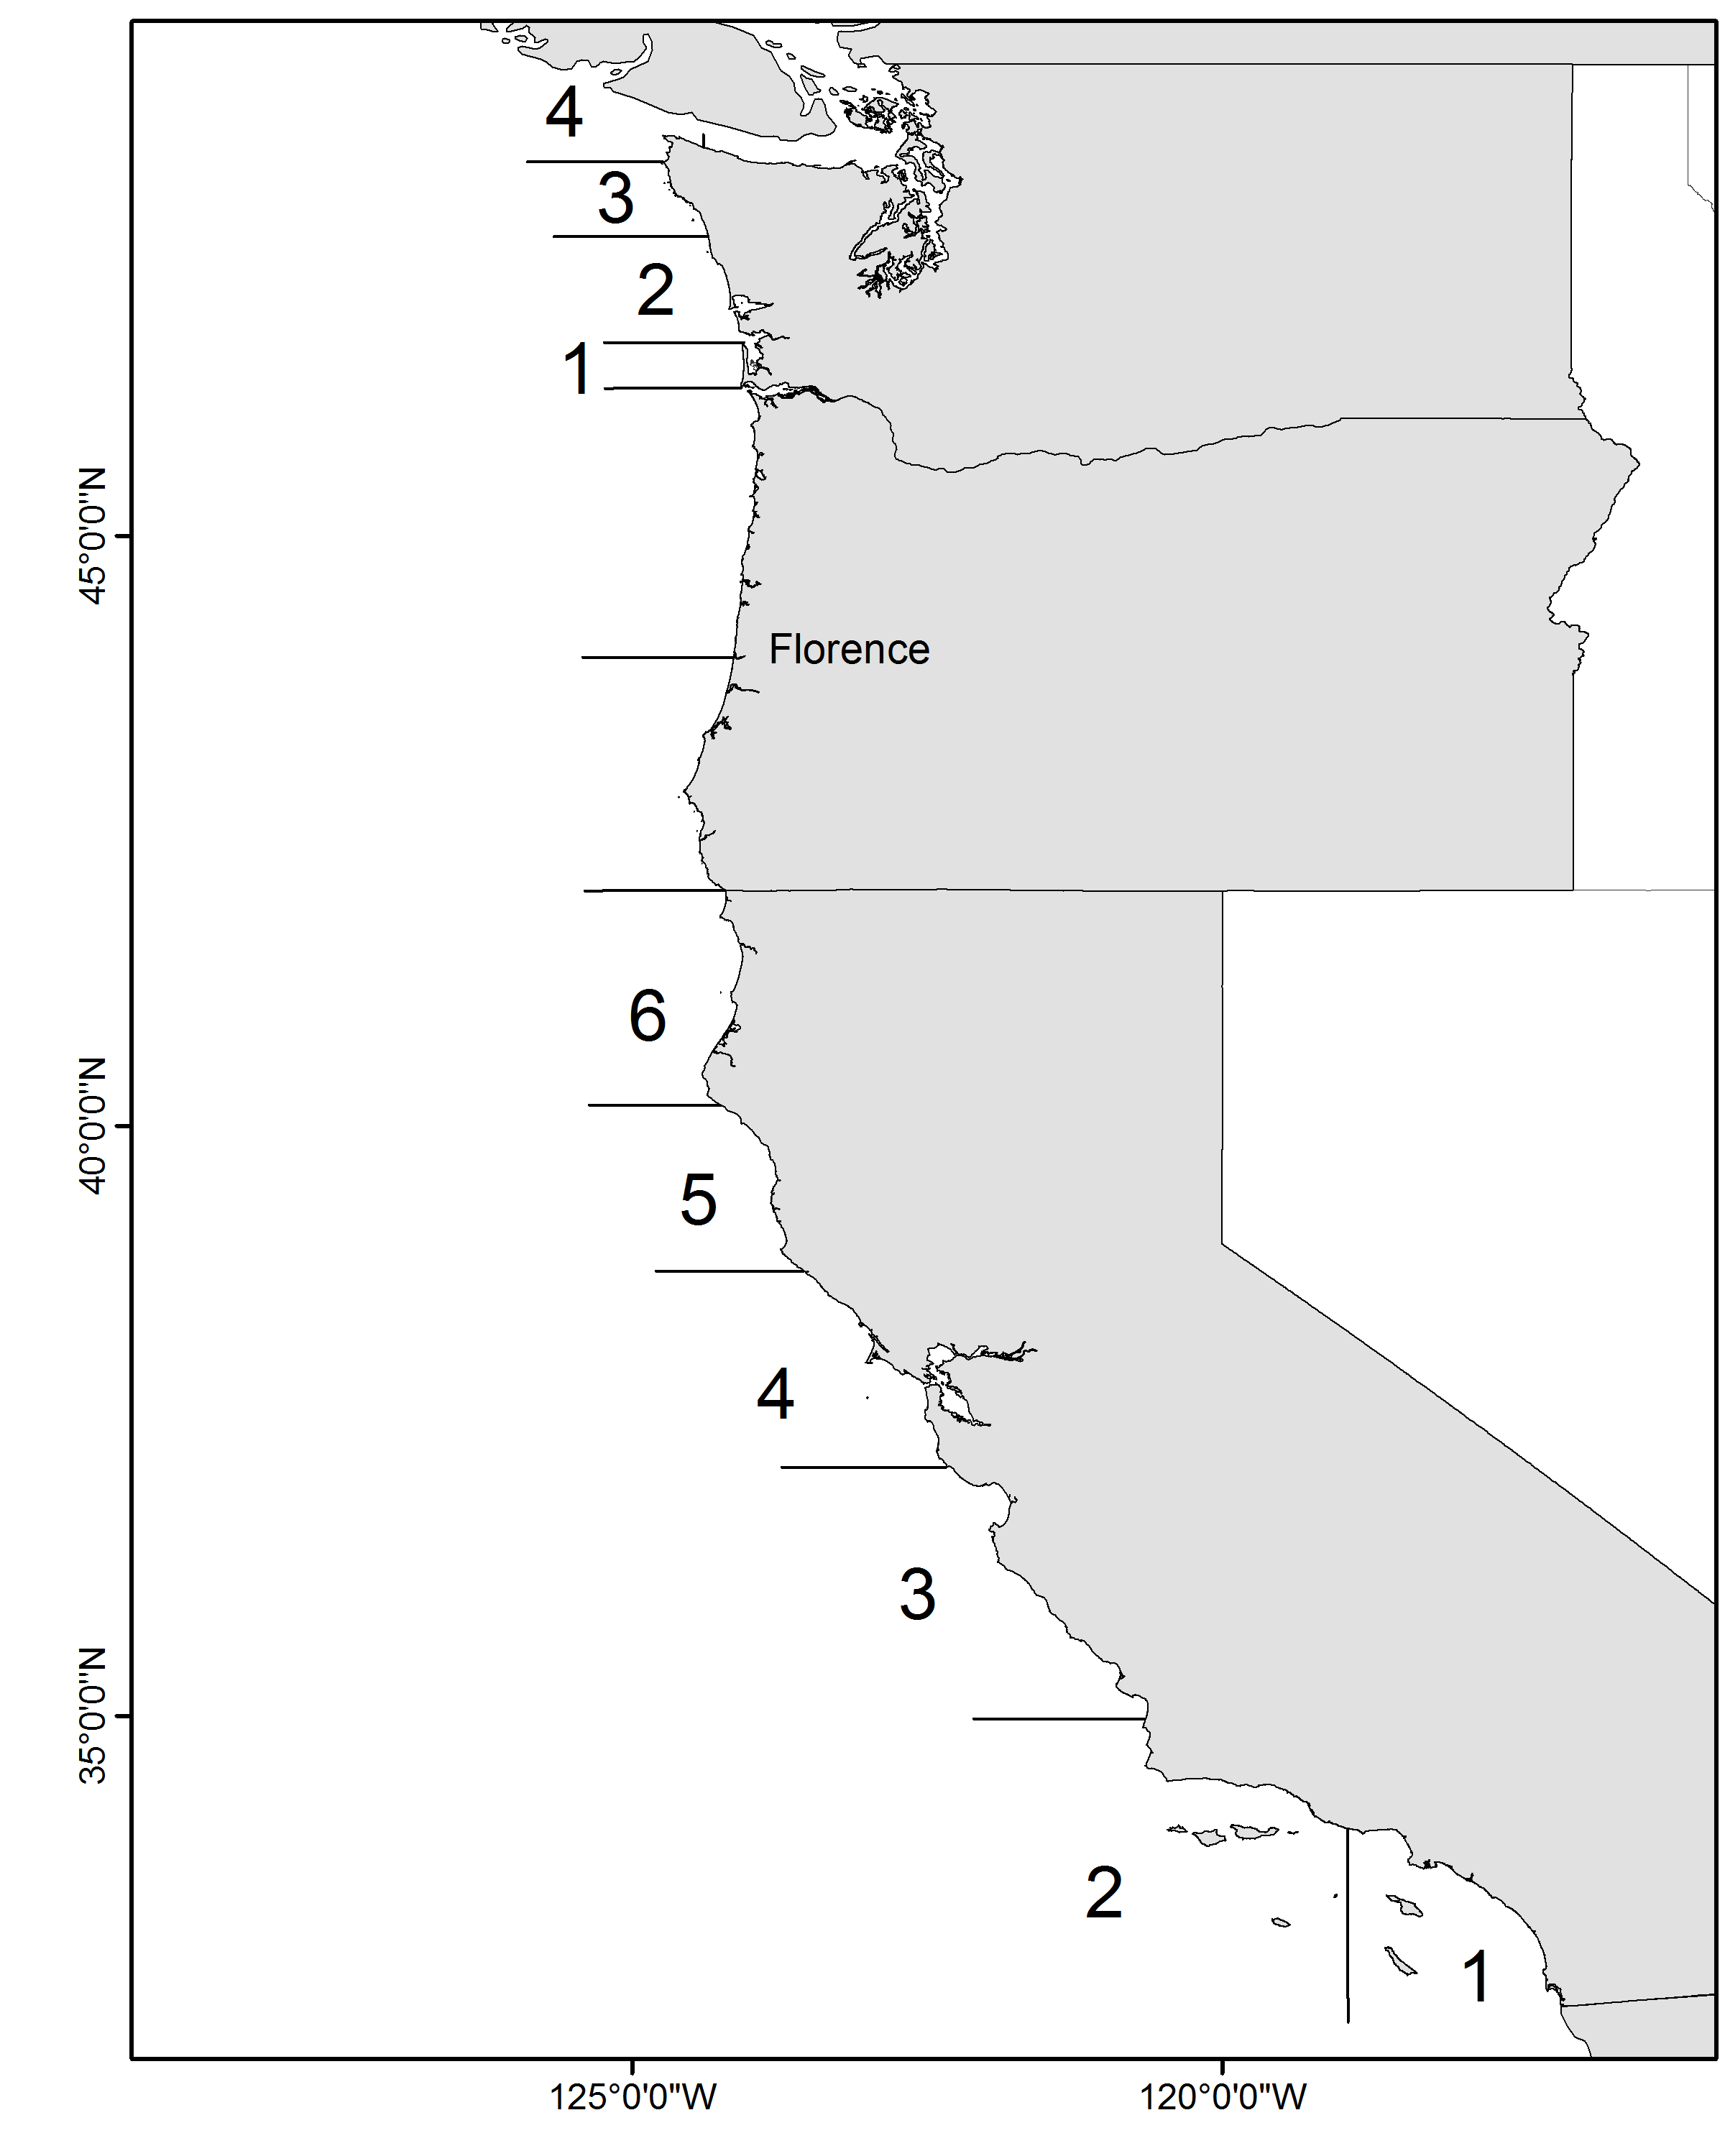
\includegraphics{Figures/boundary_map.png}
\caption{Map showing the state boundary lines for management of the
recreational fishing fleets. CRFS Districts 1-6 in California are
presented as well as the WDFW Recreational Management Areas in
Washington. Florence, OR is shown as a potential location of model
stratification. \label{fig:boundary_map}}
\end{figure}

\begin{figure}[htbp]
\centering
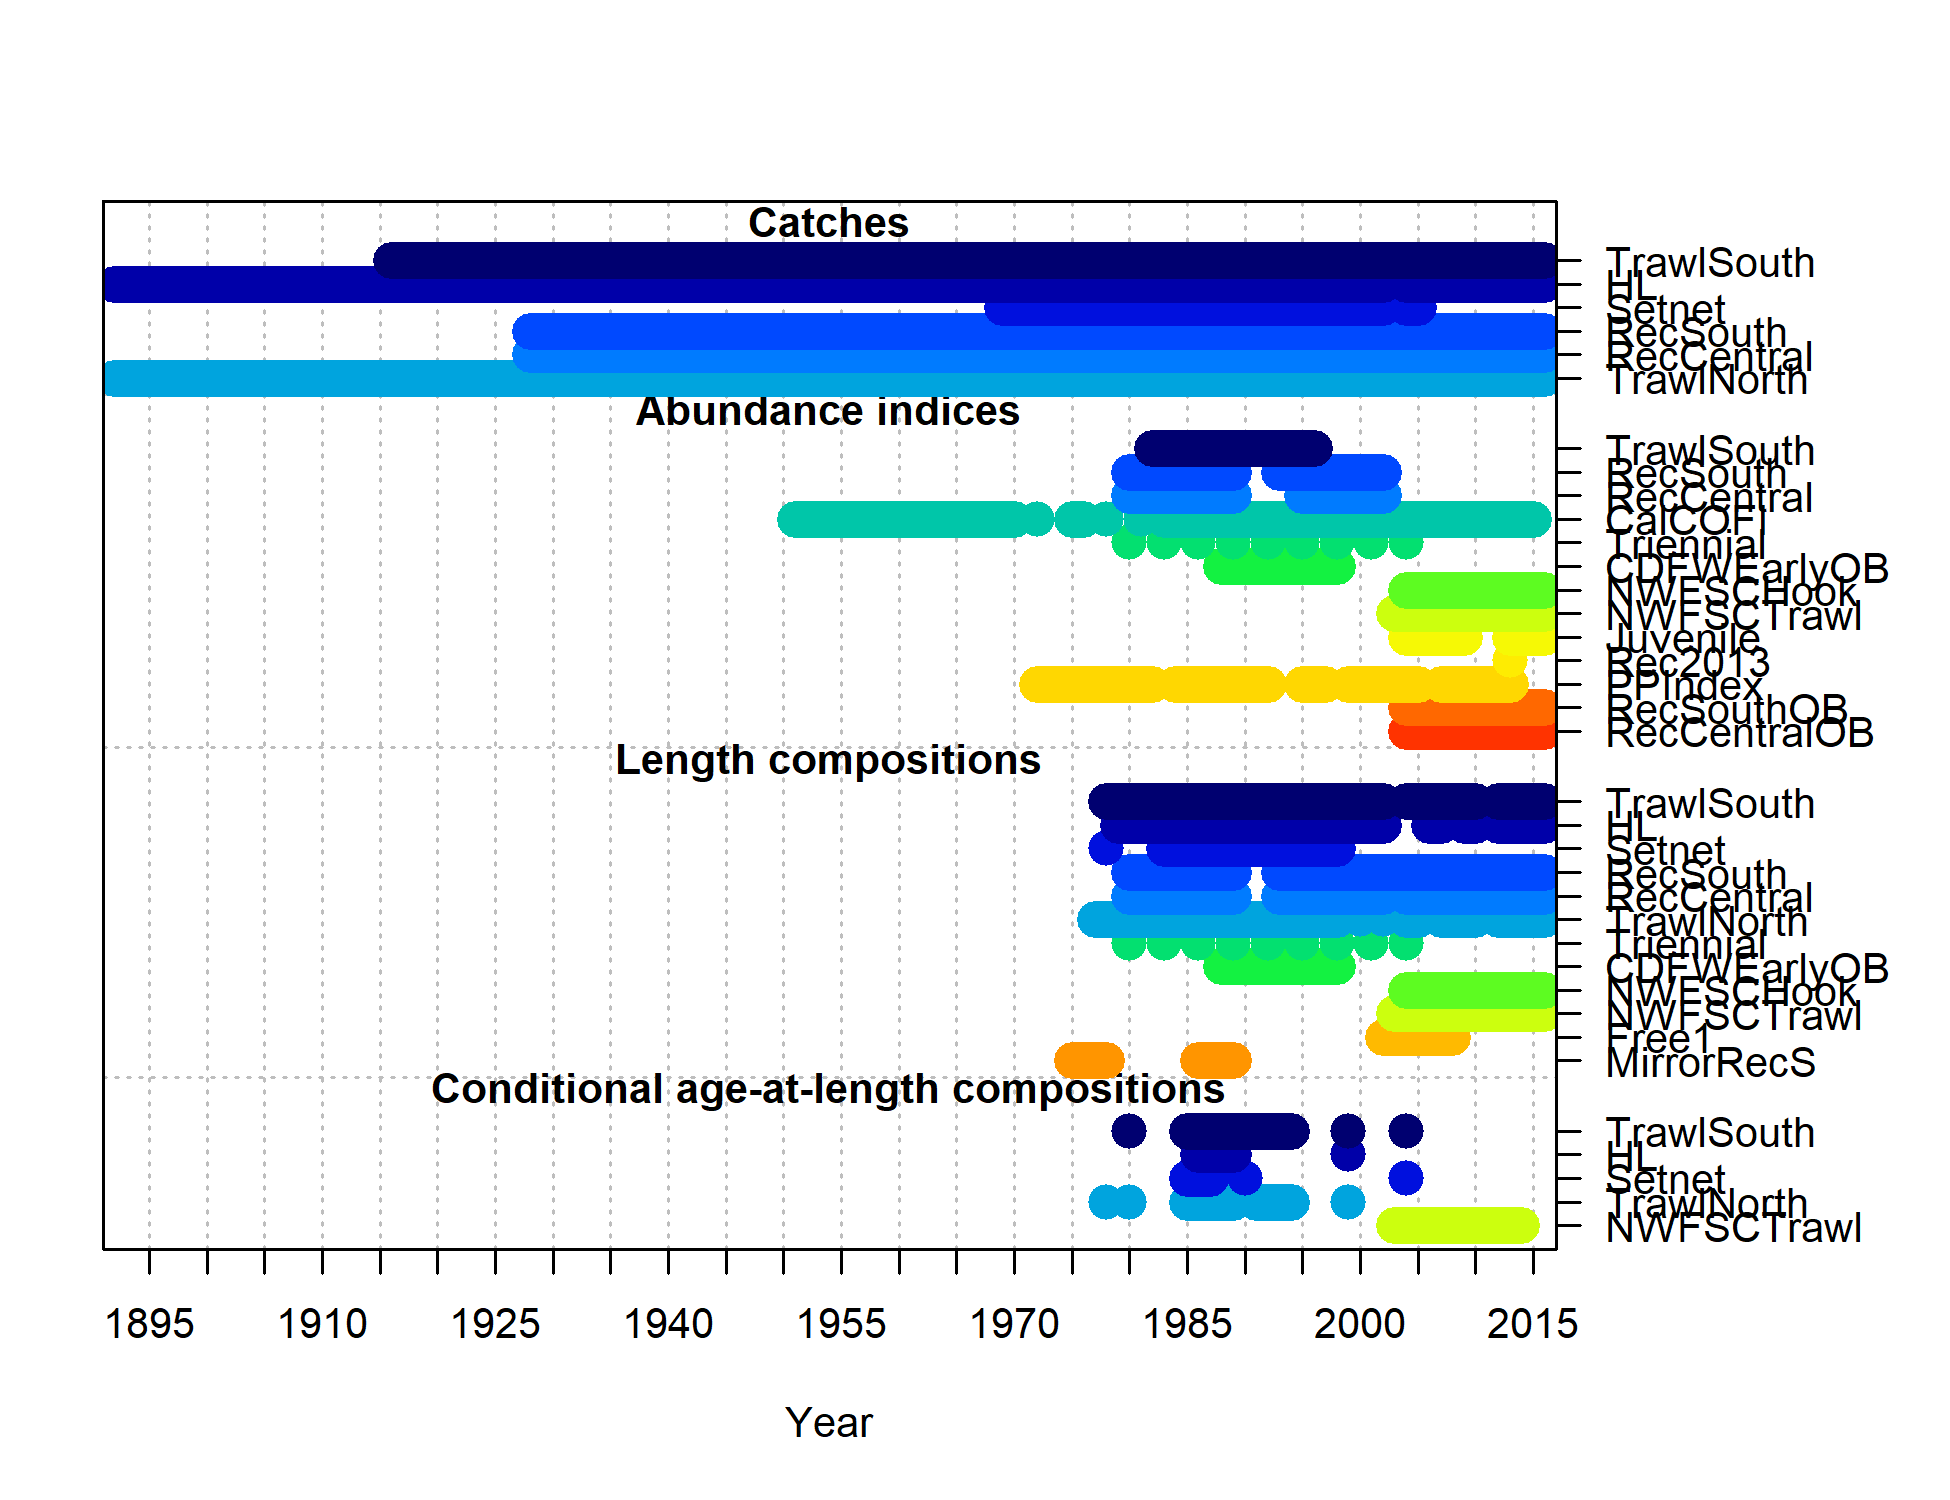
\includegraphics{r4ss/plots_mod1/data_plot.png}
\caption{Summary of data sources used in the northern assessment.
\label{fig:data_plot}}
\end{figure}

\FloatBarrier

\FloatBarrier

\FloatBarrier

\FloatBarrier

\FloatBarrier

\FloatBarrier

\begin{figure}[htbp]
\centering
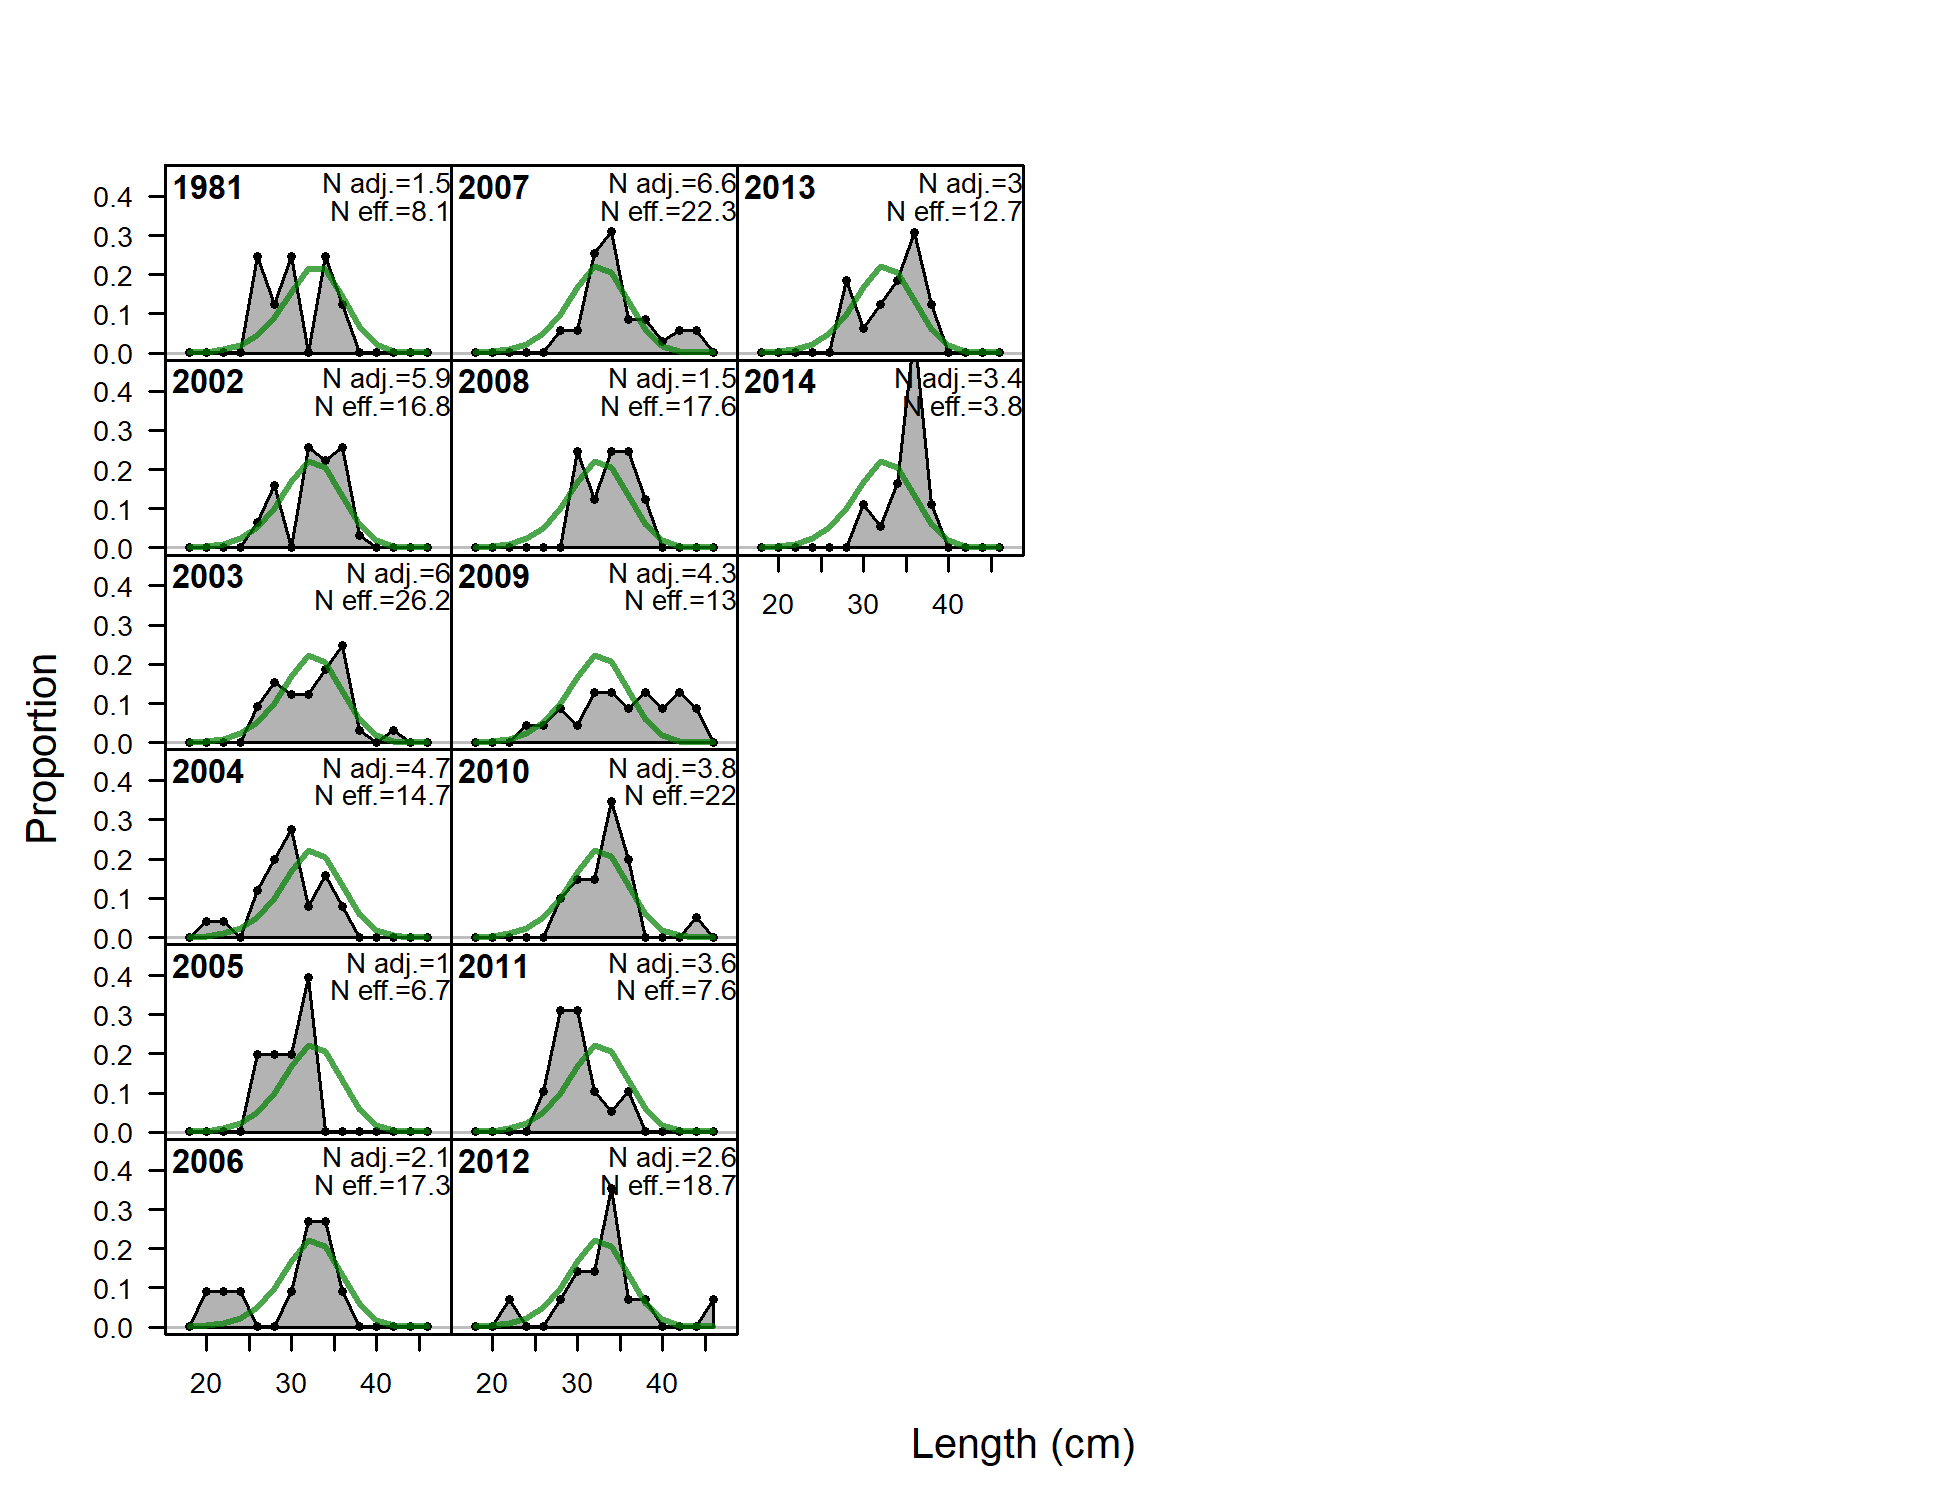
\includegraphics{C:/StockAssessment_template/r4ss/plots_mod1///comp_lenfit_flt1mkt2.png}
\caption{length comps, retained, 1\_WA\_SouthernWA\_Rec\_PCPR
\label{fig:mod1_1_comp_lenfit_flt1mkt2}}
\end{figure}

\begin{figure}[htbp]
\centering
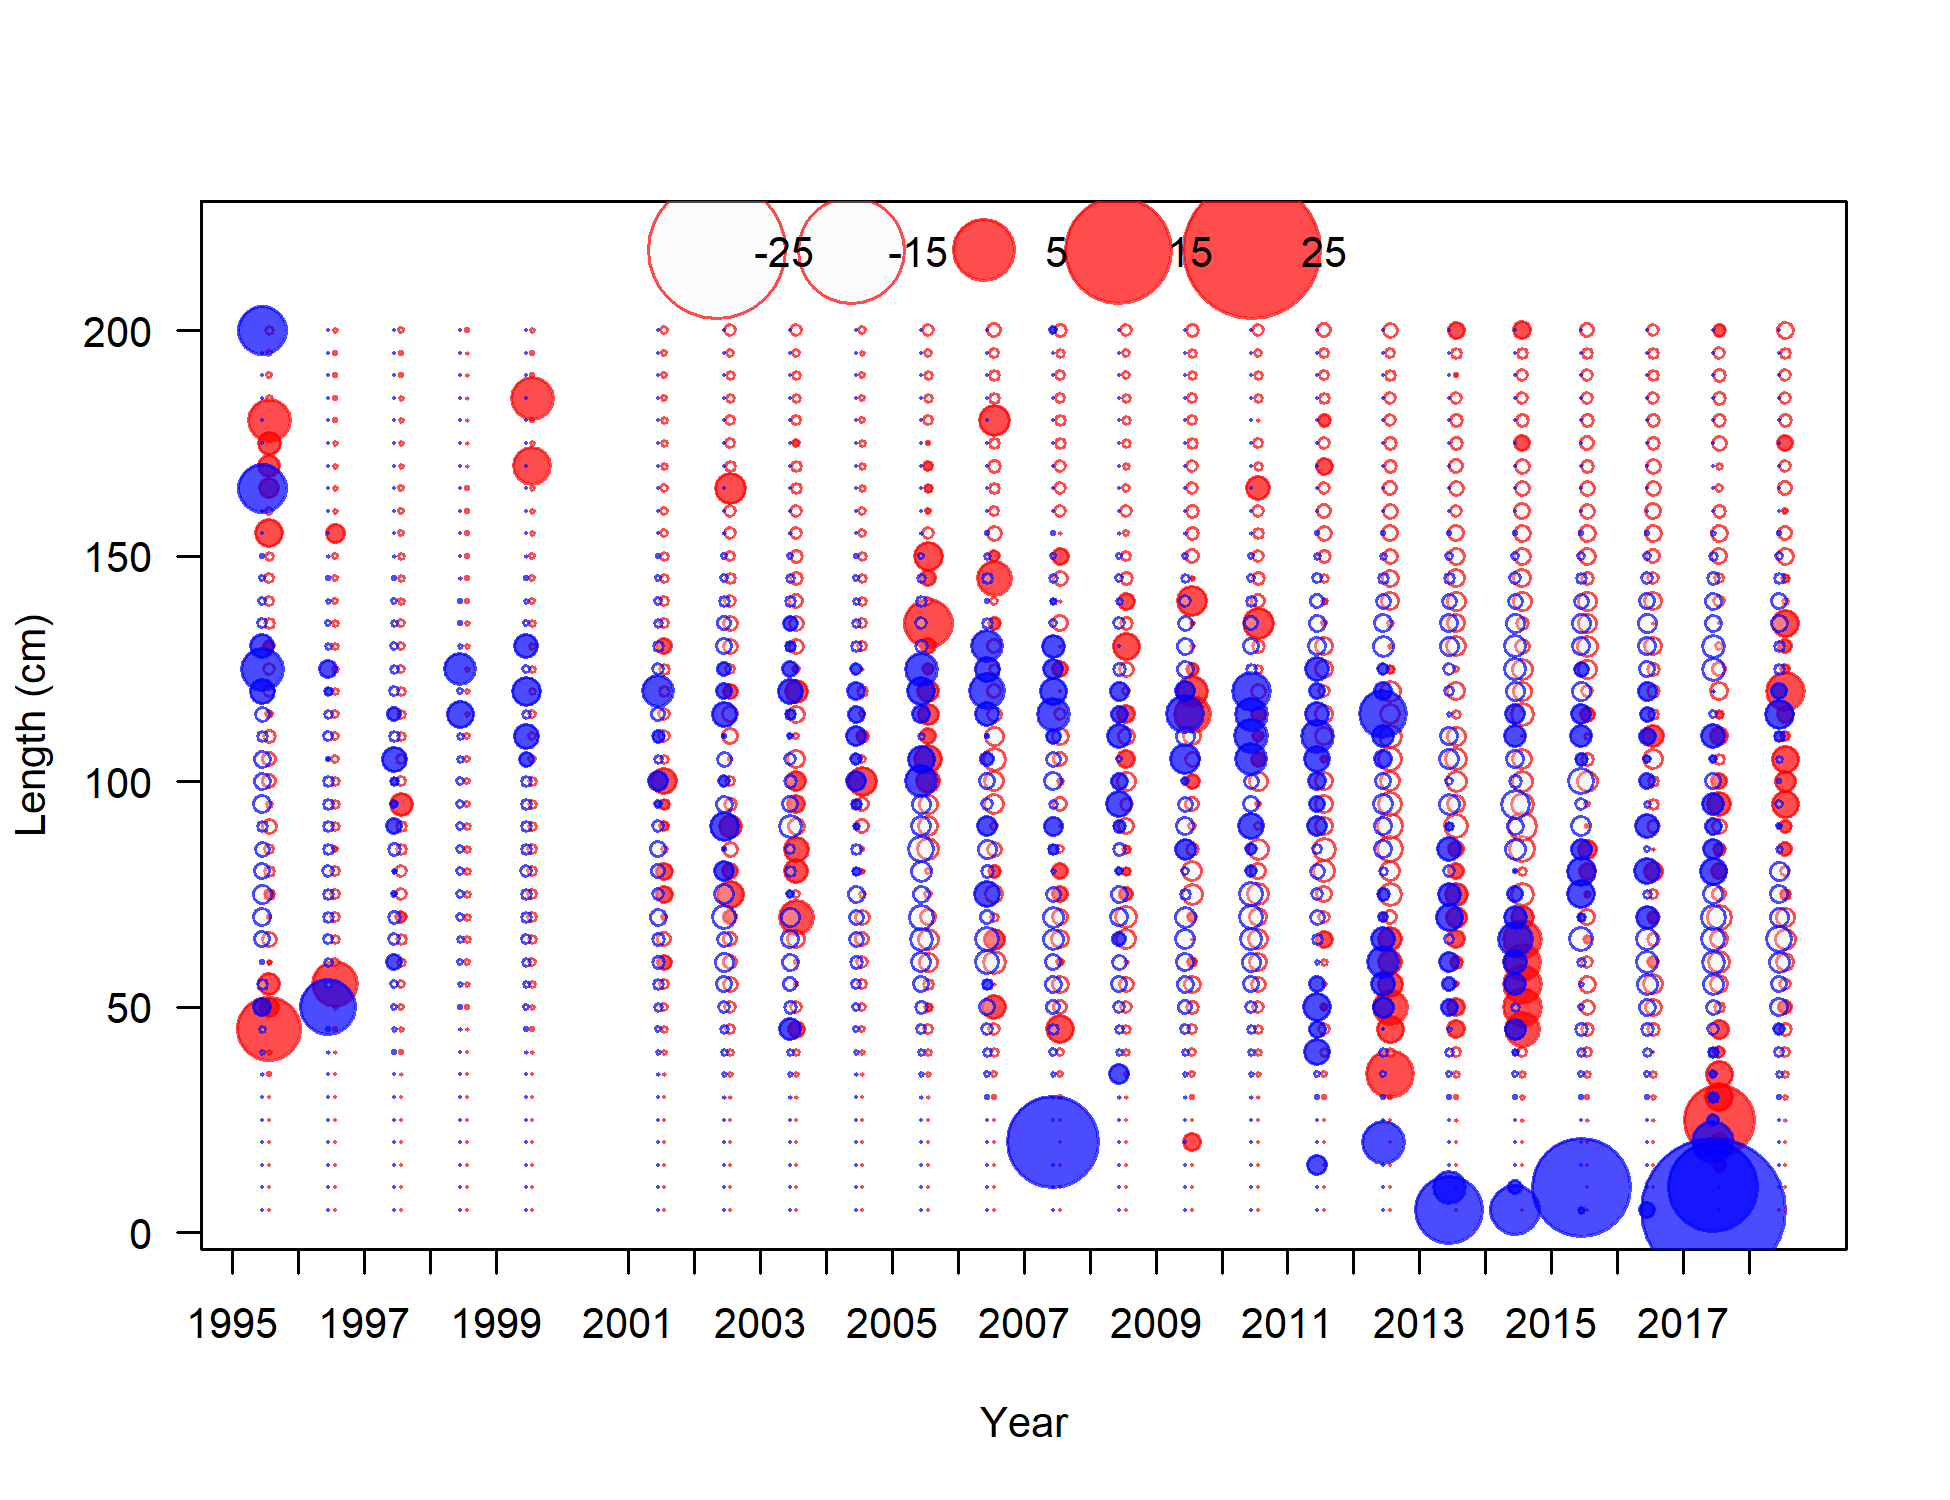
\includegraphics{C:/StockAssessment_template/r4ss/plots_mod1///comp_lenfit_residsflt1mkt2.png}
\caption{Pearson residuals, retained, 1\_WA\_SouthernWA\_Rec\_PCPR
(max=4.76)\\
Closed bubbles are positive residuals (observed \textgreater{} expected)
and open bubbles are negative residuals (observed \textless{} expected).
\label{fig:mod1_2_comp_lenfit_residsflt1mkt2}}
\end{figure}

\begin{figure}[htbp]
\centering
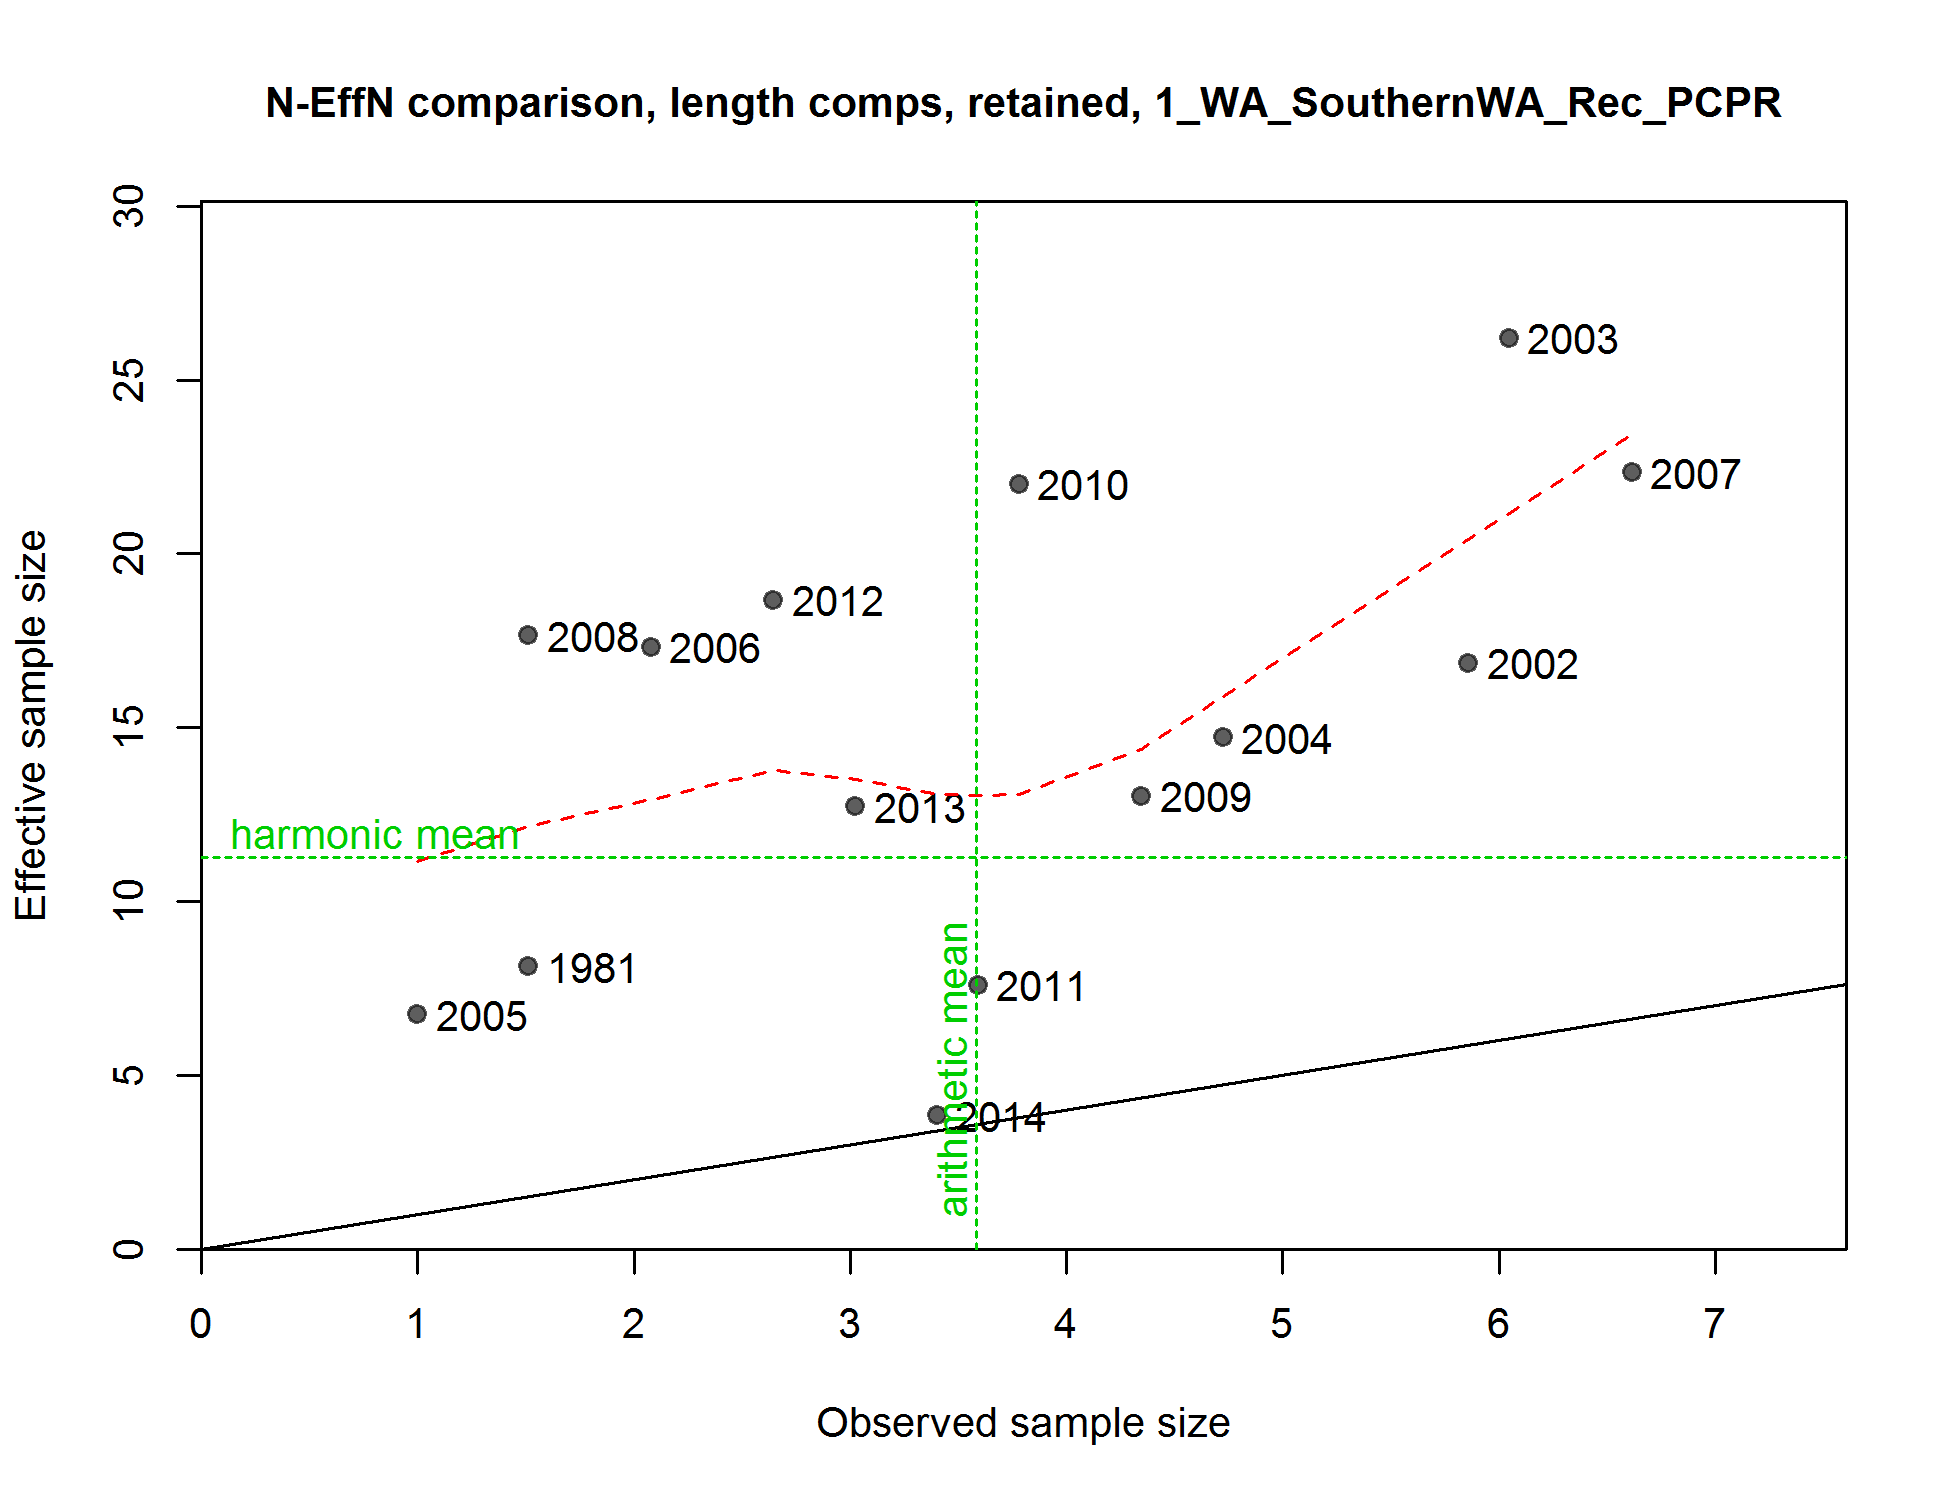
\includegraphics{C:/StockAssessment_template/r4ss/plots_mod1///comp_lenfit_sampsize_flt1mkt2.png}
\caption{N\_EffN comparison, length comps, retained,
1\_WA\_SouthernWA\_Rec\_PCPR
\label{fig:mod1_3_comp_lenfit_sampsize_flt1mkt2}}
\end{figure}

\begin{figure}[htbp]
\centering
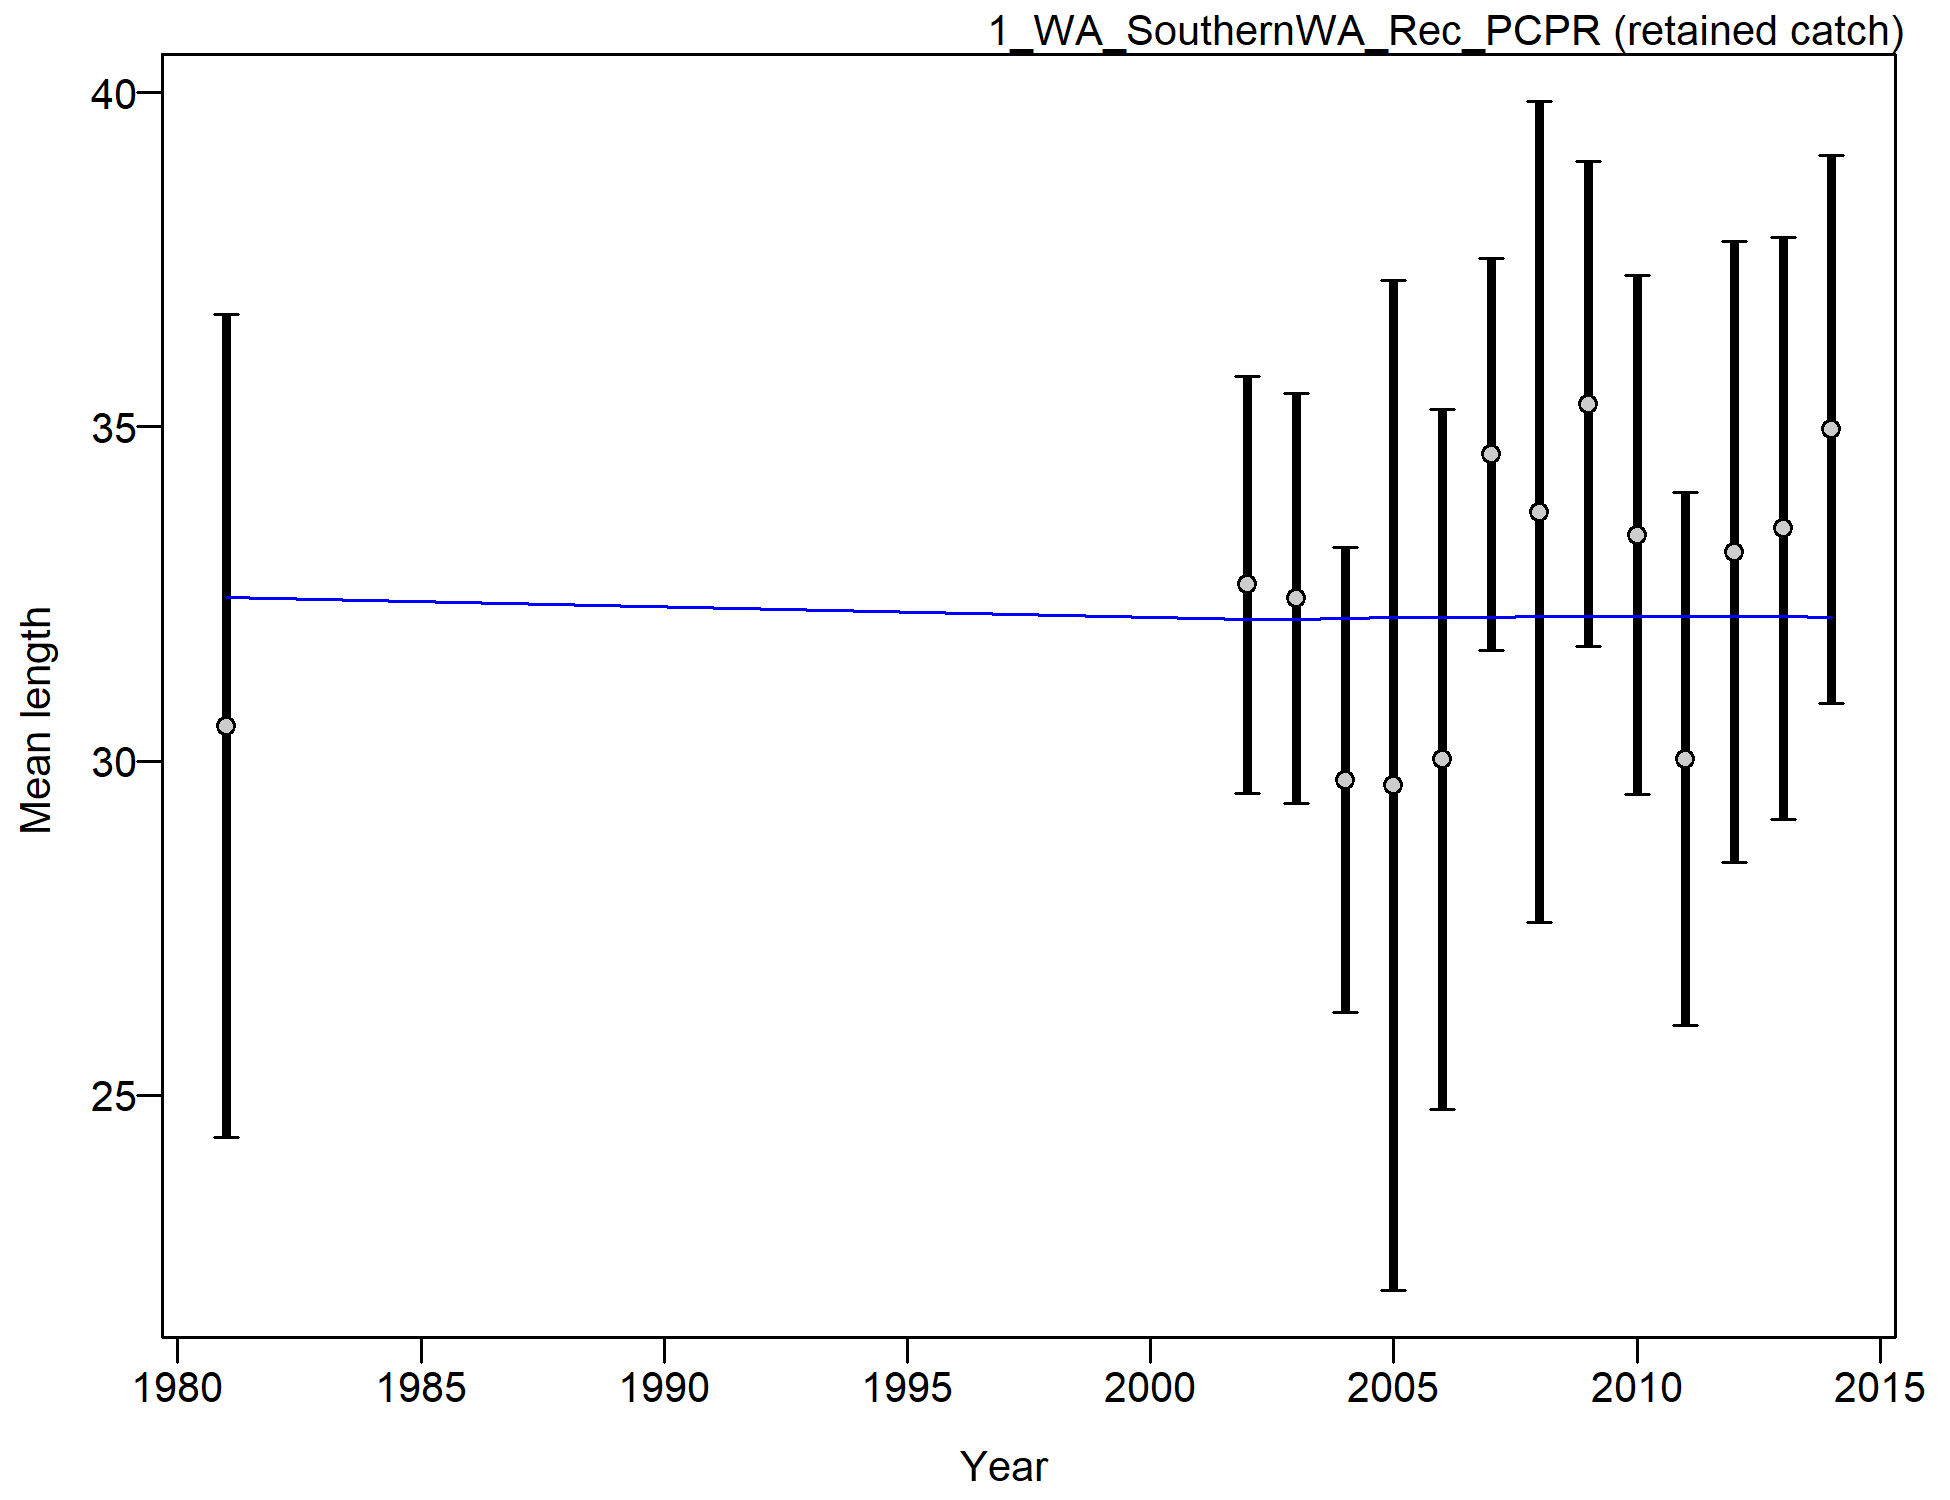
\includegraphics{C:/StockAssessment_template/r4ss/plots_mod1///comp_lenfit_data_weighting_TA1.8_1_WA_SouthernWA_Rec_PCPR.png}
\caption{Francis data weighting method TA1.8
1\_WA\_SouthernWA\_Rec\_PCPR Suggested sample size adjustment (with 95\%
interval) for len data from 1\_WA\_SouthernWA\_Rec\_PCPR: 0.9991
(0.6902\_2.2209)
\label{fig:mod1_4_comp_lenfit_data_weighting_TA1.8_1_WA_SouthernWA_Rec_PCPR}}
\end{figure}

\begin{figure}[htbp]
\centering
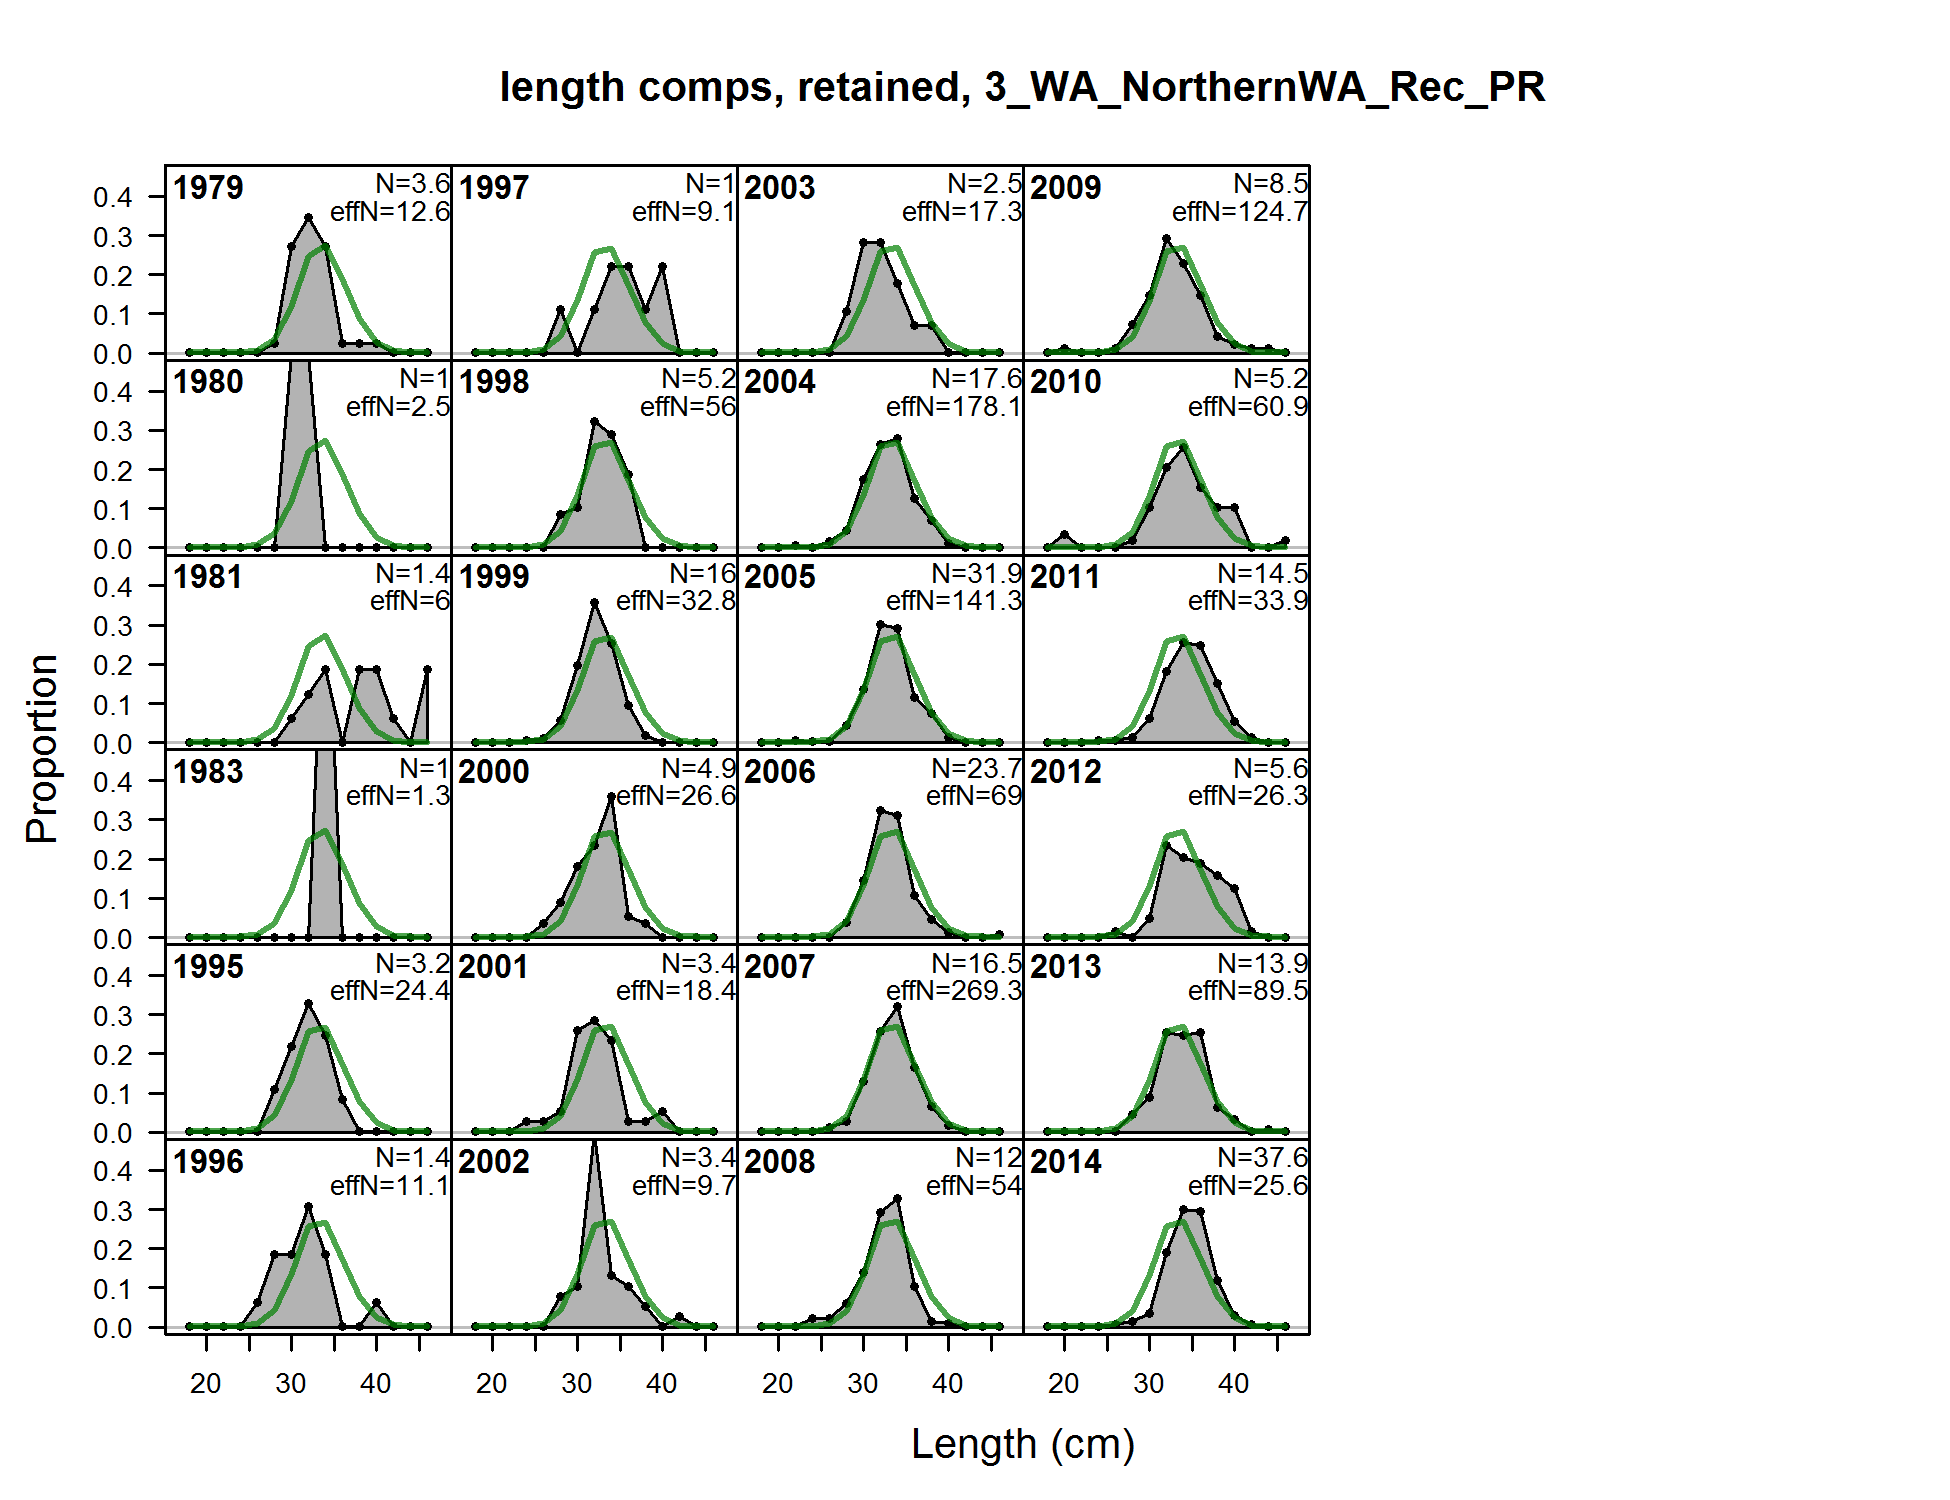
\includegraphics{C:/StockAssessment_template/r4ss/plots_mod1///comp_lenfit_flt3mkt2.png}
\caption{length comps, retained, 3\_WA\_NorthernWA\_Rec\_PR
\label{fig:mod1_5_comp_lenfit_flt3mkt2}}
\end{figure}

\FloatBarrier

\FloatBarrier

\FloatBarrier

\FloatBarrier

\FloatBarrier

\FloatBarrier

\FloatBarrier

\newpage

\section*{References}\label{references}
\addcontentsline{toc}{section}{References}

\renewcommand{\thepage}{}

\hypertarget{refs}{}
\hypertarget{ref-Alverson1964}{}
Alverson, D.L., Pruter, a T., and Ronholt, L.L. 1964. A Study of
Demersal Fishes and Fisheries of the Northeastern Pacific Ocean.
Institute of Fisheries, University of British Columbia.

\hypertarget{ref-vonB1938}{}
Bertalanffy, L. von. 1938. A quantitative theory of organic growth.
Human Biology \textbf{10}: 181--213.

\hypertarget{ref-Dick2009}{}
Dick, E. 2009. Modeling the reproductive potential of rockfishes
(\emph{Sebastes} spp.). PhD Dissertation, University of California Santa
Cruz.

\hypertarget{ref-Francis2011}{}
Francis, R. 2011. Data weighting in statistical fisheries stock
assessment models. Canadian Journal of Fisheries and Aquatic Sciencies
\textbf{68}: 1124--1138.

\hypertarget{ref-Hamel2015}{}
Hamel, O. 2015. A method for calculating a meta-analytical prior for the
natural mortality rate using multiple life history correlates. ICES
Journal of Marine Science \textbf{72}: 62--69.

\hypertarget{ref-Harry1961}{}
Harry, G., and Morgan, A. 1961. History of the trawl fishery, 1884-1961.
Oregon Fish Commission Research Briefs \textbf{19}: 5--26.

\hypertarget{ref-Love2002}{}
Love, M., Yoklavich, M., and Thorsteinson, L. 2002. The rockfishes of
the northeast Pacific. University of California Press, Berkeley, CA,
USA.

\hypertarget{ref-McAllister1997}{}
McAllister, M.K., and Ianelli, J.N. 1997. Bayesian stock assessment
using catch-age data and the sampling - importance resampling algorithm.
Canadian Journal of Fisheries and Aquatic Sciences \textbf{54}(2):
284--300.

\hypertarget{ref-Methot2015}{}
Methot, R.D. 2015. User manual for Stock Synthesis model version 3.24s.
NOAA Fisheries, US Department of Commerce.

\hypertarget{ref-Miller1965}{}
Miller, D., and Gotshall, D. 1965. Ocean sportfish catch and effort from
Oregon to Point Arguello, California July 1, 1957-June 30, 1961. State
of California, The Resources Agency Department of Fish and Game, Fish
Bulletin \textbf{130}.

\hypertarget{ref-Pikitch1988}{}
Pikitch, E., Erickson, D., and Wallace, J. 1988. An evaluation of the
effectiveness of trip limits as a management tool. Northwest and Alaska
Fisheries Center, National Marine Fisheries Service, US Department of
Commerce.

\hypertarget{ref-Rogers1992}{}
Rogers, J., and Pikitch, E. 1992. Numerical definition of groundfish
assemblages caught off the coasts of Oregon and Washington using
commercial fishing strategies. Canadian Journal of Fisheries and and
Aquatic Sciences \textbf{49}: 2648--2656.

\end{document}
